\begin{abstract}
TODO The abstract goes here...
\end{abstract}



%*****************************************************************************
%*****************************************************************************
\chapter{Introduction}
%*****************************************************************************
%*****************************************************************************
\section{Motivation}
Imagine you're meeting with your friends at a factory site to take part at a new game. On the floor, you find a piece of paper. Someone has written something on it, apparently in great haste: "They are everywhere! They are fast, intelligent! But they are not human anymore! Don't let one of them touch you or you'll become one of them! I've heard of a safe house, where you are supposed to take shelter from them. And I've hidden some weapons, with which you may stun them. I've marked the places on this map." Below, there's a link to a website, showing a map. While we are watching the linked map with our smartphones, a yelling horde of scary looking people ran up to us.
 
This is a game I played with some of my friends a couple of years ago. Let's call it "The Running Dead". Many other games like this come out these days. Games, in which the player has to physically move to succeed in the game. They are called \emph{exergames}. A popular example is Pok\'{e}mon GO. An important part of these games is the location-based content that comes along with them. For the game described above, it's the map with the marked stashes. For Pok\'{e}mon GO, it's the locations of Pok\'{e}Stops and gyms. The creation of this content is one of the big challenges today. To be able to play such a game in more than just one distinct place, there also has to be content available for these locations. It isn't fun to play The Running Dead in London, whereas the stashes have only been marked in Mainz. Nor wouldn't there be so many people playing Pok\'{e}mon GO, if one had to go to a big city each time to visit a Pok\'{e}Stop. Letting a game designer place all this content is usual, but very expensive in time and money. For this reason, this thesis presents a new approach to dynamically create content - on the basis of real-world vehicles.

\section{Challenges}
This thesis is dedicated to three domains: Pervasive games, vehicle recognition and augmented reality. In each of these domains, this thesis faces challenges and proposes and discusses solutions.

Since there is an app created along with this thesis to prove the later proposed concept, one challenge is to use motivators to attract people to play and move. Therefore, other exergames are explored and used motivators are discussed. Motivators can either be distinct aspects of the gameplay or utilized technology. Another challenge in this domain is to investigate, in which way to include vehicles as generic markers into the game.

VMMR (building dataset, training classifier, tuning parameters, multiplicity and ambiguity issues as siddiqui mentions)
 
AR on mobile device (vision-based approach (marker-based or marker-less), or alternative) and how to use it in a reasonable manner

\section{Thesis Outline}
This thesis is structured as follows:
\begin{itemize}
  \item Chapter \ref{ch:stateOfTheArt} discusses the state of the art of both, pervasive games and automatic vehicle recognition. For the pervasive games, a short historic overview is given and subgenres are listed. Finally, some examples are presented.
  
  For the automatic vehicle recognition, some different types of vehicle recognition are discussed, until the VMMR and different realizations are investigated in more detail.
  \item Chapter \ref{ch:concept} presents the concept of the mobile exergame \emph{RacecAR GO}, that is developed along with this thesis and uses vehicles as generic markers.
  \item Chapter \ref{ch:implementation} presents the server-client-architecture of RacecAR GO as well as some implementation details of the components, described in chapter \ref{ch:concept}. At the end of this chapter, the performance of the implemented VMMR system is discussed.
  \item A prototype of the RacecAR GO has been evaluated by some testers over 21 days. Chapter \ref{ch:evaluation} is about the setup and discusses the results of the evaluation critically.
  \item Chapter \ref{ch:conclusion} shortly recapitulates what has been the motivation of this thesis and what has been done and accomplished after all. Additionally, it gives an outlook of what could be the next steps to continue with this work.
\end{itemize}





%*****************************************************************************
%*****************************************************************************
\chapter{State of the Art}\label{ch:stateOfTheArt}
%*****************************************************************************
%*****************************************************************************
\section{Overview}
In this chapter, the history and the state of the art of pervasive games in general and exergames in special will be presented. Popular representatives like \emph{Ingress}\footnote{\url{https://www.ingress.com/}} or \emph{Pok\'{e}mon GO}\footnote{\url{http://www.pokemongo.com/}}, published by Niantic\footnote{\url{https://www.nianticlabs.com/}}, will be looked at.

Additionally, some interesting approaches about vehicle recognition
%(TODO low: and number plate region detection)
will be discussed as the concept presented in this thesis also includes automatic vision-based vehicle recognition.

\section{Pervasive Games}
\subsection{Definition}
Although the term pervasive gaming is becoming more and more popular within the last years, its definition is still vague \citep{nieuwdorp2009pervasive}. One is calling them a new type of digital games that combine game reality and physical reality within the gameplay \citep{Lankoski:2004:CSP:1028014.1028083}. Another definition says, that it is a game, in which the game world exists beside the everyday environment and that never stops but surrounds the player 24 hours a day \citep{sotamaa2002all}.
\citeauthor{nieuwdorp2009pervasive} defined pervasive games as special type of game that emphasizes the relation between reality and game \citep{nieuwdorp2009pervasive}.

There is some consensus in those definitions, such as the importance of the relation between the reality and the game world. But instead of bringing up another definition to compete with the other ones, this thesis compiles definitions of some works to define the boundary of pervasive games, as fitted for this thesis' scope.

A definition that tries to comprise the bottom line of many other definitions was made by \citeauthor{hock2014augmented}: \emph{"A pervasive game is an overlay of the real world where it (the overlay) is persistently present. It takes place in physical environments and its gameplay interacts with or is in some way related to parts of the real world. It thereby blurs the boundaries between reality and virtuality. It ideally integrates smoothly into its user's everyday life where it ideally is omnipresent which means that the user should be able to play it at any time in any place"} \citep{hock2014augmented}.


\subsection{Beyond Traditional Games}
\citeauthor{montola2005exploring} tried to approach the definition problem by investigating all kinds of games that have been classified as pervasive games for different and not unique reasons. He found out, that there is no single common denominator of those reasons. But regarding the magic circle of play, each of these games broke out of this circle in a distinct manner \citep{montola2005exploring}.

\subsubsection{The Magic Circle of Play}
\citeauthor{huizinga1955homo} defines a play as \emph{some activities} in \emph{some places} that are considered playfully by the players to belong to the game and not to reality \citep{huizinga1955homo}. Traditionally, a game takes place at \emph{"certain spaces, at certain times, by certain players"} \citep{montola2005exploring}. This is referred to as the magic circle of play.

For a pervasive game, this circle does not have a rigid border but a "permeable membrane where conventional meanings, psychological artifacts and environments, and players alike can slip through" \citep{nieuwdorp2005}. In relation to the magic circle of play, another definition for a pervasive game is \emph{"a game that has one or more salient features that expand the contractual magic circle of play socially, spatially or temporally."} \citep{montola2005exploring}

In the following, each of the named dimensions, in which pervasive games expand the magic circle of play, are described.

\subsubsection{Spatial Expansion}
This means, that the location, where the game can be played at, is unclear or unlimited \citep{montola2005exploring}. Thinking of the example from the beginning of this thesis, that game may have started at a factory site, but the actual spread of the zombies is unclear and could be unlimited.

Montola notes that there are challenges with this kind of expansion, causing people to play the game on unwanted places like hospitals or creating hazardous situations in traffic \citep{montola2005exploring}.

\subsubsection{Temporal Expansion}
In classic games, a play session has a well defined start and end time. Pervasive games can break these limits. Not only does the temporal expansion obfuscate the start and end time of a game, it also blurs the border between everyday life and gaming by leaving the player in the dark about if he is playing at the moment or not \citep{montola2005exploring}.

\emph{"Boring moments of life can be enchanced by any mobile game, but temporal expansion reaches even the moments of not-playing"}, because \emph{"any action could be a game action"} \citep{montola2005exploring}.

\subsubsection{Social Expansion}
The social expansion obfuscates the boundary of playership \citep{montola2005exploring}. Thinking back to the example of \emph{The Running Dead} in the beginning of this thesis, it wasn't clear who is a participant and who isn't. A noninvolved person could have watched a persecuted player and could have tried to help him. So the noninvolved person would become a participant without even knowing about it himself.

\subsubsection{Subcategories of Pervasive Games}
There are many subcategories of pervasive games, such as immersive games, serious games or exergames, to name a few. Immersive games combine spatial, temporal and social expansion. In this genre, it's hard to differentiate games from non-games, because everything can be seen as an immersive game \citep{mcgonigal2003}.

Serious games are, simply said, more than fun \citep{sawyer2008serious}. They blend education and entertainment together in one game experience \citep{ritterfeld2009serious}. The term education is not limited to a specific domain but can be all kinds of added value other than pure entertainment and fun. \citeauthor{gobel2010serious} call it a broad spectrum of application domains ranging from training, simulation and education to sports and health \citep{gobel2010serious}.

The last two domains form the subcategory of exergames. Because exergames are a subject of this thesis, the next section dedicates to that genre in more detail.

\begin{figure}[bth]
  \centering
        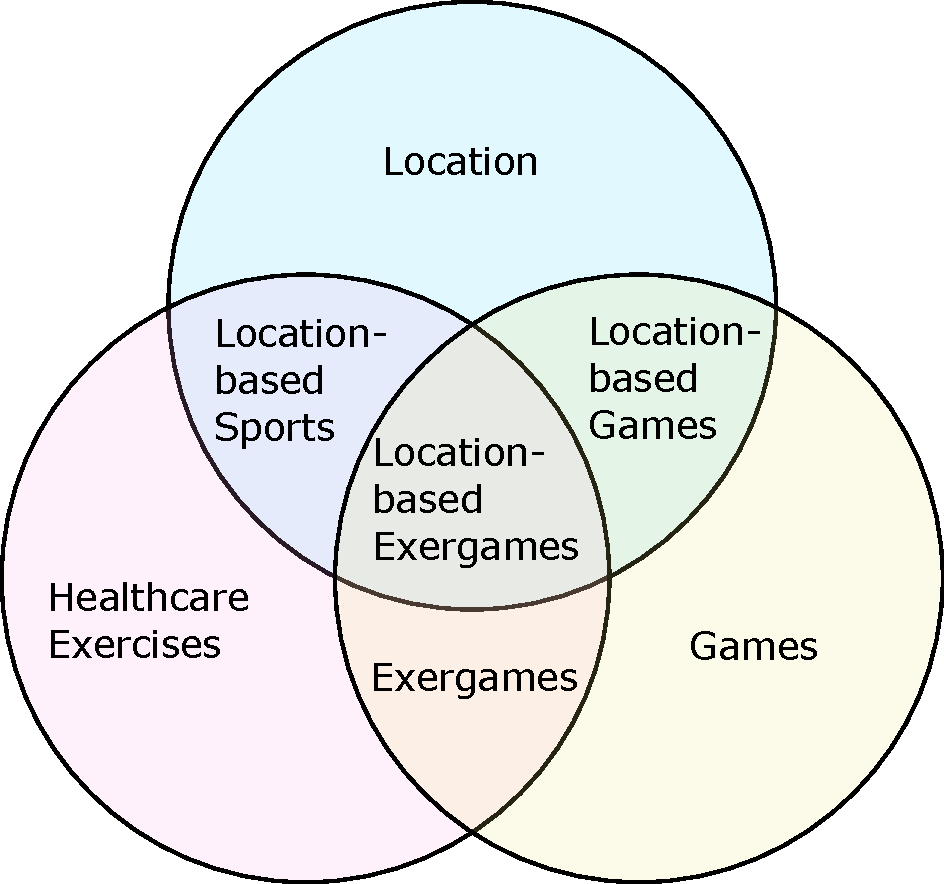
\includegraphics[width=.55\linewidth]{gfx/exergame_context}
        \caption{Context of Exergames}
        \label{fig:exergameContext}
\end{figure}

\subsection{Exergames}
A subcategory of serious games then again are exergames \citep{gobel2010serious} \citep{knoll2014urban}. As shown in figure \ref{fig:exergameContext}, exergames are games with healthcare exercises as added value. The term \emph{exergame} is constructed from the words \emph{exercise} and \emph{videogame} \citep{bogost2007persuasive}.

The target of an exergame is to combine physical activity with fun of play. During the gameplay, the health aspect is not primarily focused but only a side-effect of playing the game. \emph{"The training effect is secondary and nevertheless achieved"} \citep{knoll2014urban}. An example for an exergame is \emph{Dance Dance Revolution} (DDR) \footnote{\url{http://www.ddrgame.com/}}. DDR is available for multiple platforms, as the Nintendo Wii, the PlayStation or the Xbox. The player stands on a platform with arrows printed on it. When the screen shows an arrow (corresponding to the rhythm of a played song), the player has to step on the matching arrow on the platform. \citeauthor{bogost2007persuasive} says about this game, that it produces exercise as an emergent outcome of play itself \citep{bogost2007persuasive}.

A user of the Nintendo Wii \footnote{\url{http://wii.nintendo.de/}} wrote: "Video games can [be] and are a great way to have exercise and not even know you are burning calories" \footnote{\url{http://www.gamespot.com/forums/nintendo-fan-club-1000001/wii-sports-weight-lossyesits-real-25576131/}}. Debra Lieberman found out that there is growing evidence of exergames helping people to stay fit and to manage their weight if they frequently play them \citep{Lieberman06dancegames}.

So the challenge of an exergame is to keep the player motivated to do sports. As in the example at the beginning of this thesis (\emph{The Running Dead}), we all ran away when the mob of zombies came running towards us. We did not think of doing sports in that moment. Maybe some even did not think of playing a game. Our only thought was to escape.

\subsubsection{Mobile Exergames}
Digital games are mostly completely experienced through a fixed screen. This is an obstacle to immerse into a game \citep{cheok2002touch}, because the player is bound to his chair and his perception is usually only stimulated by the computer screen and a sound system. In pervasive games, the interface is no longer bound to a fixed screen and to common computer periphery like a mouse and a keyboard. The player rather interacts with real world objects and real persons \citep{nieuwdorp2009pervasive}, whereas the interface of the game isn't well defined. Any real world object could be a game object, and any real person could be a participant \citep{montola2005exploring}.

There is a special type of exergames, the mobile exergames, in which the player is not bound to a desktop or to a classical game board to play the game. Mobile exergames are played with a mobile device (such as a smartphone or a portable video game console). They are usually played outside and often use the location of the player to track the progress of the exercise. In most cases, the player has to move to succeed in the game, such as in Pok\'{e}mon GO or StreetConqAR (which are described in more detail in chapter \ref{sec:examples}).

These games do not take place at special locations like in a gym, a laboratory or at home, separated from the real world. They are played everywhere such as on the way to school or work, at work itself, after the lunch time, after work with your kids or whenever and wherever the player (or the game, as said above for pervasive games with temporal expansion) wants to. The aim is a transformation of the player's everyday environment into a world in play \citep{nieuwdorp2009pervasive}.


\subsection{Evolution of Location-based Games}\label{sec:locationBasedGames}
In the previous chapters, different types of pervasive games have been presented. Many of them depend on the current location of the player, e. g. Ingress or Pok\'{e}mon GO (see section \ref{sec:examples}). This kind of games uses the current location as a basic part of the gameplay. Without the exact location, a player of Ingress could not conquer a portal and a hunter on the prowl for Pok\'{e}mons would not find one nor would he find a Pok\'{e}stop to retrieve useful items. Concluded, these games would be absolutely unplayable without being able to track the location of the player with a reasonable accuracy.

Using GPS, this is only possible since May 2, 2000, when the \emph{Selective Availability} was turned off. Selective Availability was a service to prevent civilians to perceive a better GPS accuracy than a 100 meters radius, reserving better accuracy for the military only. Since it was disabled, the GPS location is accurate to a few meters for anybody\footnote{\url{http://www.gps.gov/systems/gps/modernization/sa/data/}}.

Suddenly, many location based games came up. For example, the term \emph{Geocaching} was formed during that time to describe a hunt for treasures (the \emph{geocaches}) in the real world \citep{Geocaching}. To find these geocaches, their locations are marked on a virtual map via GPS.

A few years later, the popular 80s game \emph{Pacman}\footnote{\url{https://en.wikipedia.org/wiki/Pac-Man}} was transferred into a real-life version named \emph{Pac-Manhattan} \citep{Pac-Manhattan}, using GPS sensors to track the position of the players.

With the launch of the iPhone in 2007, an era began where people always have a device at hand that is not only capable of tracking the GPS location but that is also powerful enough to run useful apps on it. This caused another hype of location-based applications.

One of it, heavily relying on GPS-based location, is Foursquare\footnote{\url{https://foursquare.com/}}. The service makes personalized recommendations of places to a user. These recommendations depend on the user's current location and his profile. The service exists as a mobile app and as a website. Providing an iPhone app in 2009, Foursquare was one of the pioneers that combined a serious mobile application with a location-based service.

At that time, the app had a check-in feature to virtually check into specific locations. This game-like feature motivated users to visit different places to check-in and leave a Tip.

Another location-based game, that became very popular, is \emph{Ingress} (see chapter \ref{sec:examples}). Ingress also uses the smartphones of the players to track their location and let them conquer virtual entities (named portals), that have been spread over the world.

A new member of location-based games is \emph{Pok\'{e}mon GO} (see chapter \ref{sec:examples}). Like in Ingress, players have to move in the real world, using their smartphone to discover virtual objects (like Pok\'{e}mons or Pok\'{e}stops), that have been placed on real-world locations.

The real-world locations, where entities are placed in the virtual world, play an important role for these games. They have to be well-chosen to fit the purpose of the game and the respective gameplay. These special locations are called \emph{anchors}.

\subsubsection{Anchors}\label{sec:anchorsStateOfTheArt}
For location-based games, the real world is overlain by the virtual game world. Anchors are well defined positions, where these two worlds are blurred \citep{hock2014augmented}. The word \emph{anchor} has been introduced by \citeauthor{hock2014augmented}. In literature, there is no fixed term for this. Other works also refer to this as \emph{artifacts} \citep{reid2008design} or as \emph{(generic) markers} \citep{matyas2008designing}, as named in the title. This thesis uses the term anchor \citep{hock2014augmented}, because its semantic meaning describes very well what an anchor does: It anchors the virtual world into the real world. Another reason is, that the term \emph{marker} is already established in the context of augmented reality, which this thesis also relates to.

The placement of anchors is very important for a game and is directly associated with the user experience. Because anchors are those positions, where the gameplay usually takes place, players may easily be disappointed if an anchor is either too far away to reach it or if it is at a location not (without further ado) accessible for civilians (such as military areas, airports or the ocean). So anchors have to be placed in a way that they are accessible for all players.
Another thing is the content, that is linked to an anchor. For example, the game \emph{Escape From the Tower} \citep{EscapeFromTheTower} lets its players reenact the escapes of some popular prisoners from the London Tower. Therefore, anchors are placed all over the tower and its surroundings with associated media. At a prison cell, this media tells the player something about the prisoner. On the staircase, the media is related to a fled, that occurred. If the content does not fit to the respective location, players will soon quit the game.

\citeauthor{reid2008design} classifies the way, anchors are placed, into three categories, that will be explained in the following.

\paragraph{User-placed at Runtime}
With this method, the user places his own anchors. For this, the game has to provide some kind of editor, with which the user creates the content he needs to play the game.

The advantages of this method are, that the game can be played everywhere, because it does not depend on predefined anchors. Another advantage is, that users can create the anchors such that they fit their individual needs. In Twostone \footnote{\url{https://play.google.com/store/apps/details?id=de.tu.darmstadt.uhg}} for example, the player plays a stone-eating caterpillar that moves on a maze-like virtual track while the player moves in the real world. To win the game, the caterpillar named "Twostone" has to eat all stones, that are spread all over the track while escaping from some monsters, that try to catch it. The game includes an editor, wherewith the user can design a track by walking along the paths, where the track should be created and placing anchors at corners. The game can thus be played anywhere. Also, highly motivated and sporty players can build their own large tracks covering the whole city, whereas beginners are able to design a small one for a short sport unit during the lunch time.

Drawbacks of this method are, that a user is not a designer and may not have the required artistic skills and knowledge to produce qualitative anchors. And much less in a small amount of time \citep{carraca2014procedural}.

Additionally, if the player desires for a quick sporting activity, he might rather go jogging in the park than starting to build a track.

\paragraph{Seamful Design}
With this method, the placement of anchors depends on features of the physical infrastructure. In \emph{Feeding Yoshi} \citep{reid2008design}, anchors are placed on the seams of wireless access points. In the area of a secure wireless access point, the player can find a hungry creature, a "Yoshi", whereas at unsecure wireless access points, there are plantations to plant each Yoshi's favorite fruit.

Usually, developers try to hide the limitations caused by infrastructural seams. With this method, these limitations are embedded into the gameplay \citep{broll2005seamful}.

Games using a seamful design to place anchors can be played at all locations, where the respective infrastructure exists. Therefore, the accessibility depends on the choice of the kind of the infrastructure. Nowadays, unsecure wireless access points are rather seldom, hence the gameplay of Feeding Yoshi suffers from this choice.

\paragraph{Designer-placed}
With this approach, all anchors are placed by the game designer. Due to the designer's skills and insight to the respective game, the anchors are usually well-placed and harmonize with the gameplay.

As a drawback, this method is the most static and expensive one, consuming time and money until all needed anchors are placed. As a result, most games with designer placed anchors are tailored for a specific scenario, such as \emph{Escape from the Tower} \citep{EscapeFromTheTower}, which was mentioned above. The anchors in such games are often strongly related to their location. Adapting this game for another location would involve much effort.

Additional to those categories introduced by \citeauthor{reid2008design}, this thesis names two further categories.

\paragraph{Crowd-based Placement}
Crowd-based placement of anchors is akin to user placement, with the difference that content created by the crowd is made public for everyone. This way, the game thrives on a lively crowd of users, frequently creating new content.

Twostone, that has been mentioned before, is actually relying on crowd-based anchors, because after creating a new track, a player can opt to make the track public to be used by other players. But as mentioned in the beginning, this does only work if there is a crowd creating that content. During the release of a game, it might get challenging to build up a crowd despite the fact that there is no content yet.

Another problem is, that with a crowd, there is no control of the content. After some time, the game might contain anchors at hazardous locations such as airports or highways or it might contain pictures of morally questionable content, such as swastikas or of adult kind.

Ingress uses a crowd-based placement, combined with a designer to check the content for its propriety. Nevertheless, Ingress is only playable in highly populated areas while portals (the anchors) only exist in these regions (see Ingress map in figure \ref{fig:ingressMap}). That's because users are allowed to create anchors, indeed, by taking a photo of the desired new location, marking it on a map and sending this along with a short description to the development team of Ingress. So most requests are made for regions with a lot of citizens. But it takes several weeks, until a new portal gets accepted by the designers.

\paragraph{Automatically-placed}
This scheme describes content, that is generated automatically, obeying some creation-rules. Automatic placement of anchors helps to spread them all over the world in a fraction of time and money, a designer would need.

Actually, the seamful design is a sub-scheme of automatic placement, whereas the creation-rule is to place anchors at infrastructural seams (e. g. of wireless access points).
The rule can be well-defined, such as with a procedural content generation rule, including the use of generative grammars, spatial algorithms or pseudo-random number generators \citep{carraca2014procedural}.
The rule can also be more complex like \emph{place an anchor at each gas station marked by Google Maps}, which already includes some locational context.

Automatic placement also includes \emph{random} placement. But simply placing anchors at random locations will seldomly have the result of well-placed anchors semantically fitting to their content and being accessible for everyone (e. g. oceans and deserts).

\citeauthor{hock2014augmented} proposed an automatic placement based on real-world objects, namely street name signs. In his game \emph{StreetConqAR}, the players have to conquer streets, identified by the name on their street name sign. Because StreetConqAR is similar to the game RacecAR GO, which is presented in this thesis, it's described as one of the examples in chapter \ref{sec:examples}.

The definition of an anchor says, that it is a "well-defined position". In the following, the term anchor is not only the position but also refers to the real-world object itself to describe the kind of blurring of reality and virtuality and the strong relationship between the anchor and its position. This blurring takes place via an object at a well defined position.

Later on, this thesis will define the term of a \emph{natural anchor} to solve this ambiguity (see chapter \ref{sec:anchorsConcept}).

The advantage of \citeauthor{hock2014augmented}'s approach is, that it not only saves the expanses of the a priori design of the anchors, because street name signs are already there. Also the spreading of these signs is very useful for a location-based exergame. There are very few populated regions with no street name signs.

\subsection{Augmented Reality Games}\label{sec:augmentedRealityStateOfTheArt}
I still remember my astonishment when I first saw the virtual shark, rising behind Marty McFly and then snapping at him in \emph{Back to the Future Part II}. The movie was released in 1989, wherein Marty watches the shark during his visit of the future year of 2015.

Although the year 2015 has passed, today's technology is not able to produce such a holographic shark as it has been predicted by the movie (nor has the movie \emph{Jaws 19} been released, the shark was advertising for).
Nevertheless, if Marty would wear some smartglasses today, he could see the shark indeed, with the help of augmented reality.

Augmented reality (AR) means augmenting perceived real-world elements with virtual media in realtime. This virtual media can be text, images, but also 3D objects or sound.

The term \emph{augmented reality} exists for many years now. There have been moments in the past, the technology seemed likely to experience the hype, many people are waiting for. But a big hype never happened (at least until the time of writing this thesis, May 2017).

Today, there are some popular apps that use AR, such as Snapchat \footnote{\url{https://www.snapchat.com/}} (which tracks the user's face and augments it with some fancy extras like a dog's snout with matching ears and tongue) or Pok\'{e}mon GO (described as one of the examples in chapter \ref{sec:examples}).

Also Apple and Facebook start to invest into this technology. Apple CEO Tim Cook even denotes augmented reality and virtual reality as potential cornerstones of the company's future. Also the coming iPhone 8 is said to be equipped with technology customized for AR\footnote{\url{http://appleinsider.com/articles/17/03/17/iphone-8-could-herald-start-of-apples-augmented-reality-ambitions}}. Facebook CEO Mark Zuckerberg teased an upcoming games platform for AR\footnote{\url{http://www.businessinsider.de/facebook-next-big-thing-augmented-reality-mark-zuckerberg-2017-4?_ga=1.68446423.790124447.1492966107&r=US&IR=T}}.

Maybe, this technology is finally on the verge of experiencing a big hype.

\subsubsection{Variants}
There are different variants, all called AR. This starts with simply overlaying a video with information that is located at specific GPS coordinates or at a tracked marker and ends with exactly overlaying real-world objects with virtual objects, considering 3D position and pose.

The used variant depends on the use case and on the available hardware. The higher the grade of accuracy, with which the reality shall be augmented, the higher the requirements on the hardware, since AR is usually done in realtime. Whereas overlaying the camera picture with a virtual object while the player is located at specific GPS coordinates is a rather simple job for current hardware, tracking real-world objects from the camera picture and retrieving their position and orientation to blend the virtual object over it needs a powerful CPU that is capable of sophisticated computer vision algorithms. In the following, some common approaches of integrating virtual content into the real world are presented.

\paragraph{Square Markers}
Square markers are, as the name says, square pictures containing a binary pattern (see figure \ref{fig:marker}). Square markers are easy and fast to detect in a camera image and the position as well as the pose of the marker can be deduced from its binary pattern in a very efficient way. Most of the AR APIs as ARToolKit \footnote{\url{https://artoolkit.org/}} or MetaIO \footnote{\url{http://www.metaio.eu/}} provide an implementation for this kind of markers. Even current smartphones are able to track multiple square markers in realtime.

A drawback is, that the markers have to be placed in the real world beforehand. This is a disqualifier for many application fields, where the AR content has to smoothly integrate into an unprepared scene.

\paragraph{Natural Feature Tracking}
Natural Feature Tracking (NFT) refers to a technique that searches predefined features in an image. From the locations of the tracked features, the pose and location of the camera is retrieved \citep{neumann1999natural} (see figure \ref{fig:nft-tracking}).

\paragraph{Model-based Tracking}
Similar to NFT, the captured image is searched for features while these features have to match with those of a reference model. Whereas for the NFT the reference model is an image, for model-based tracking it's a 3D CAD model. The advantage is, that with a 3D model, multiple perspectives to match the reference model to the real image are supported (see figure \ref{fig:model-based-tracking}).
Because there's much literature on this subject (e. g. \citep{lepetit2005monocular}) and since this thesis' scope only touches this kind of tracking, it won't be described any further.

\begin{figure}[bth]
  \centering
        
\includegraphics[width=.2\linewidth]{gfx/jh_marker}
        \caption{Example for a square marker}
        \label{fig:marker}
\end{figure}
\begin{figure}[bth]
  \centering
        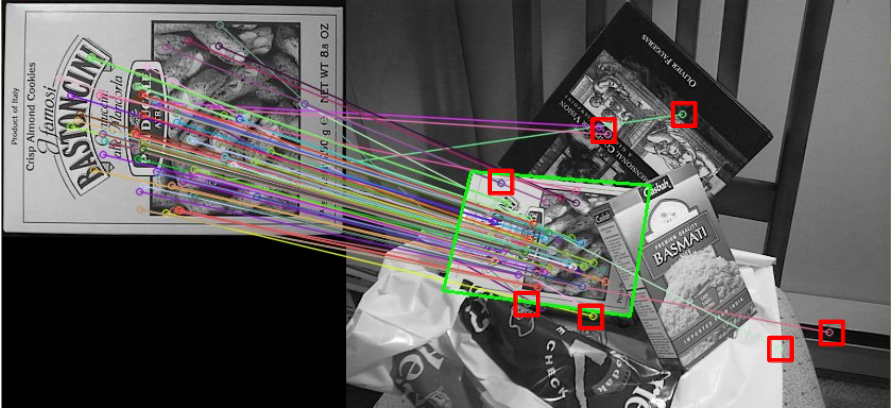
\includegraphics[width=.45\linewidth]{gfx/nft_tracking_reprint}
        \caption{Both in scene (right) and reference model (left) features are detected. Although the matching in this
example contains false positives (red boxes) the object and its transformation are estimated correctly
as its borders are marked at the right place (green). (Caption and image reprinted from \citep{hock2014augmented})}
        \label{fig:nft-tracking}
\end{figure}
\begin{figure}[bth]
  \centering
        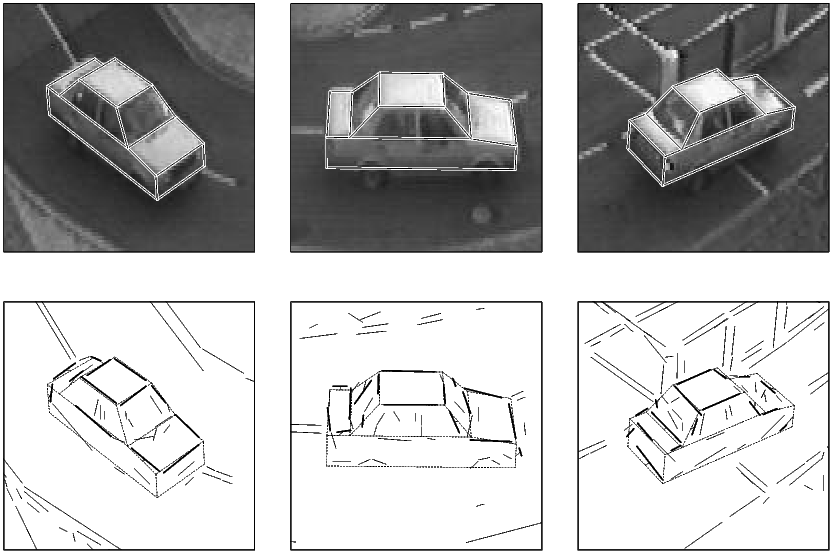
\includegraphics[width=.45\linewidth]{gfx/model_based_tracking_reprint}
        \caption{Model-based tracking: Pose estimation from correspondences between 3D model edge segments and 2D image segments. (Reprinted from \citep{lepetit2005monocular})}
        \label{fig:model-based-tracking}
\end{figure}

\subsubsection{Usage of AR in Games}\label{sec:usageOfARStateOfTheArt}
Nowadays, mobile devices used for AR are usually handheld devices (such as smartphones or tablets) or head-mounted displays (such as smartglasses). Head-mounted displays have an advantage over handheld devices, which are embarrassing, annoying, tedious to keep up and watch through and that are socially not accepted\footnote{\url{http://mobilbranche.de/2017/04/augmented-virtuelle-realitaet-facebook-f8}}. Additionally, a smartphone's hardware is limited and its camera is hardly able to capture 3D structures of the real world.

On the other hand, smartphones are common and nearly everyone will always have one at hand in the near future, whereas head-mounted displays are still a rarity.

To be smoothly integrated into everyday life, pervasive games want the player to quickly immerse into the game. Augmented reality is a technology that supports the immersion effect \citep{waern2009three}, if used in the right way. \citeauthor{wetzel2008guidelines} warn developers in their \emph{Guidelines for Designing Augmented Reality Games} \citep{wetzel2008guidelines} to not only focus on a fancy technology like AR to impress the players but to rather invest in a good user experience by a lasting gameplay.

An early example for a mobile game that uses AR is \emph{ARQuake} \citep{piekarski2002arquake}, which is an augmented reality version of the video game \emph{Quake}. It is played outside and uses AR markers.

More recent examples are the popular games \emph{Ingress} and \emph{Pok\'{e}mon GO}, that are described in detail in section \ref{sec:examples}.

Although this is a subchapter of \emph{Pervasive Games}, not each augmented reality game is a pervasive game. A game can include augmented reality technology without expanding the magic circle.

\subsection{Examples}\label{sec:examples}
In this section, representatives of one or more of the above mentioned game types (such as location-based games, exergames and augmented reality games) are presented.

The presented games have been chosen because of their close relation to the game \emph{RacecAR GO}, which is developed within this thesis.

\subsubsection{Ingress}
Ingress is a location-based mobile exergame, developed for smartphones. It was developed by Niantic and was released in 2012. Players, called \emph{agents}, have to decide to either belong to the fraction of the Enlightened or to the Resistance.

The anchors are designer placed and are called \emph{portals}, which have to be "hacked" by the players to gain points for their fraction (see figure \ref{fig:ingressGameplay}).

The portals are usually located at points of social or artistic interest, such as monuments or landmarks. In contrast to StreetConqAR (see below), these objects are of no further relevance for the gameplay.

Ingress is no augmented reality game, although it is sometimes classified as such. It mixes reality and virtuality by the use of anchors, but is does not augment the view of the physical environment.

Ingress is considered an exergame because players have to physically move to portals to succeed in the game. The game developers, however, did not seem interested in exploiting its full potential as an exergame. Players aren't motivated by the game to walk faster or farther. It is even possible to elude the health aspect completely by moving via car or bus to visit the portals, because the app does not check the speed of the player. It seems that Ingress became an exergame just by chance, since the developers figured out that it is entertaining to embed the virtual game world into the real world around the player \citep{knoll2014urban}.

Ingress is based on location data from Google Maps. Its enriched location data was used later to populate \emph{Pok\'{e}mon GO} \citep{Ingress}.

As said above, the anchors are placed by a designer. Although there exists a process for users to propose locations for new ones, which takes a few weeks to be accepted, there are many (rural) regions, where no anchors exist so far (see map in figure \ref{fig:ingressMap}). In these regions, Ingress cannot be played.

\begin{figure}[bth]
  \centering
        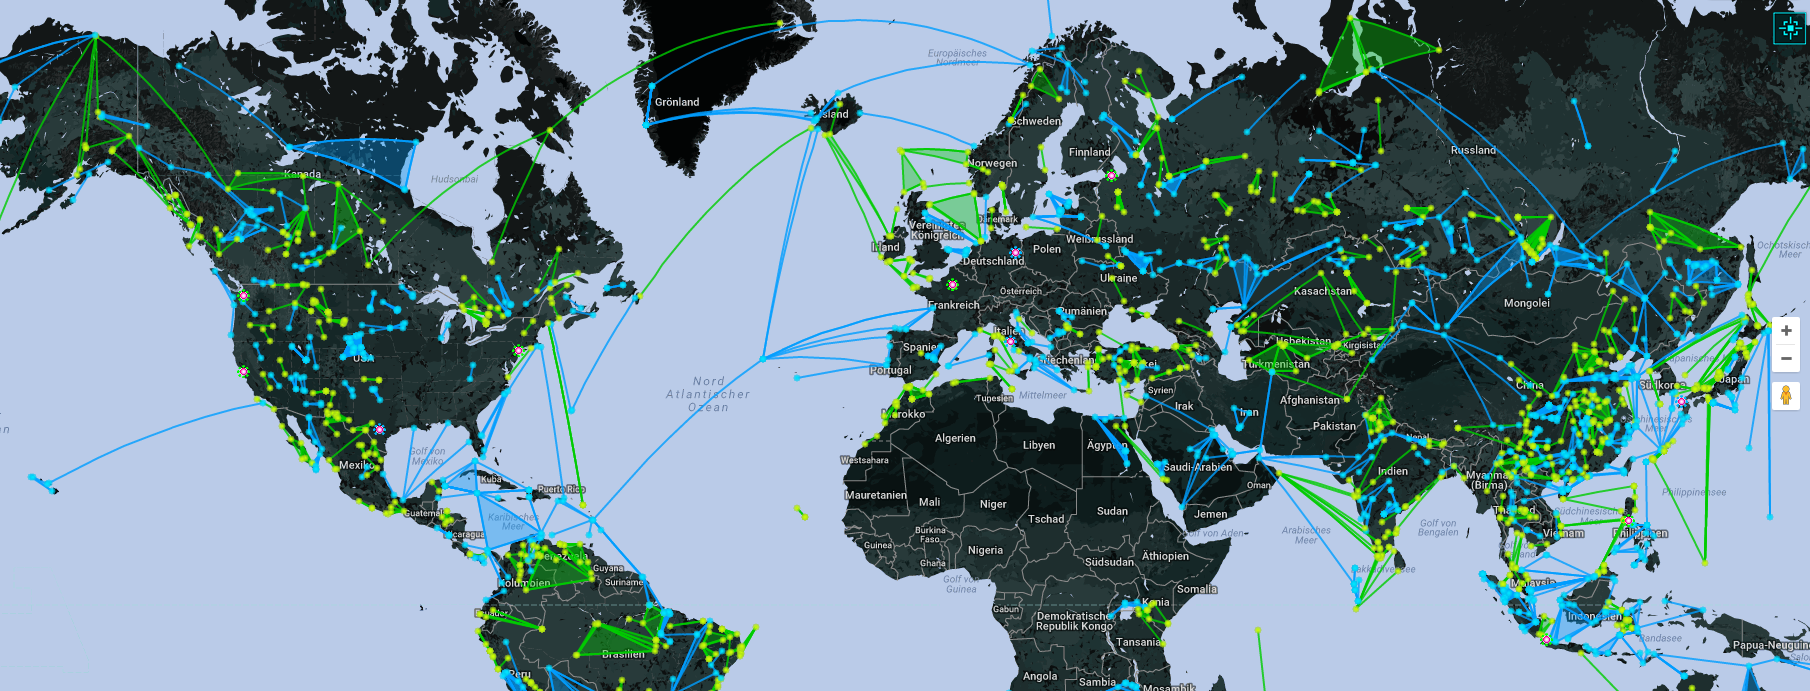
\includegraphics[width=.95\linewidth]{gfx/ingress_map}
        \caption{Screenshot of world map with Ingress portals taken with my Ingress account}
        \label{fig:ingressMap}
\end{figure}
\begin{figure}[bth]
  \centering
        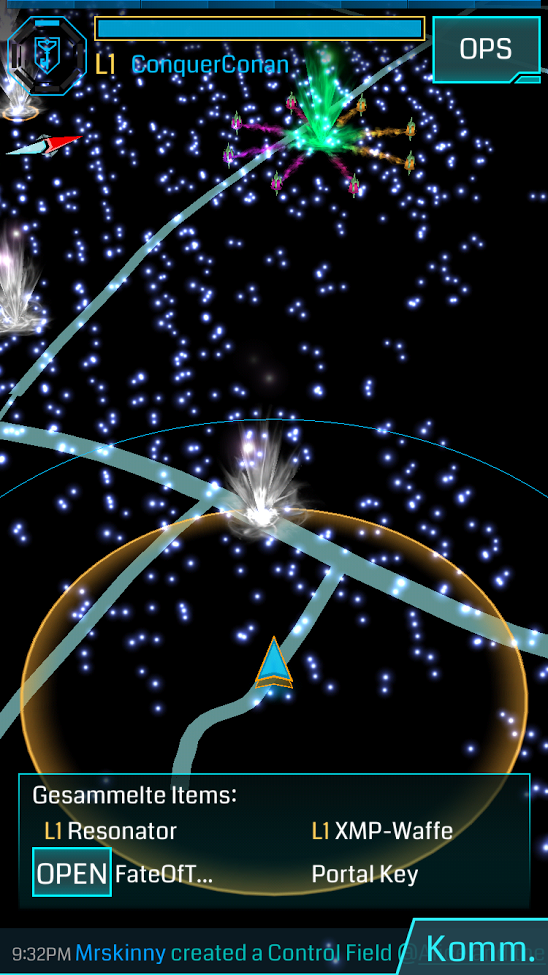
\includegraphics[width=.45\linewidth]{gfx/ingress_gameplay}
        \caption{Screenshot of playing Ingress (taken with my Ingress account)}
        \label{fig:ingressGameplay}
\end{figure}

\subsubsection{Pok\'{e}mon GO}
Pok\'{e}mon GO is a location-based augmented reality mobile exergame, developed for smartphones. It was developed by Niantic and was released in 2016. Pok\'{e}mon are fantastical creatures and first appeared in the 1990s in video and card games.

A player of Pok\'{e}mon GO becomes a Pok\'{e}mon trainer with the task to hunt up and to catch Pok\'{e}mon. Caught Pok\'{e}mon are stored in the player's Pok\'{e}dex and can be trained. In Pok\'{e}mon gyms, Pok\'{e}mon can fight against each other. There also exist Pok\'{e}Stops, where some useful items can be found.

Data gathered with Ingress was used to place gyms and Pok\'{e}Stops \citep{Ingress}. These are also marked on a map that is visible when playing the game. Pok\'{e}mon, however, are only visible through the smartphone display, if the player is physically near them. In this case, the Pok\'{e}mon is blended above the camera video in an AR manner (see figure \ref{fig:pokemonGOGameplay}).
To actually catch a Pok\'{e}mon, the player has to throw a virtual Pok\'{e}ball onto the creature. Only a well-thrown ball captures the Pok\'{e}mon. Pok\'{e}balls can be retrieved from Pok\'{e}Stops.

In contrast to Ingress, the developers emphasize the health aspect in Pok\'{e}mon GO. Though it's still possible to visit gyms and Pok\'{e}Stops by car or bus, there's a feature in the game that can only be used by walking: Brooding eggs. To brood Pok\'{e}mon eggs, the player has to walk a certain distance until the Pok\'{e}mon emerges. This distance can only be walked by feet since the app checks the movement speed of the player.

Another good thing is, that it does not really make sense to play this game inside. To succeed in the game, one has to go outside and walk around (e. g. to gather Pok\'{e}balls, to find new Pok\'{e}mon or to brood eggs).

The virtual map that displays Pok\'{e}Stops and gyms also motivates the players to move. At least it motivated myself. Seeing these locations in the near environment, I though "I'm tired from work, but there are two Pok\'{e}Stops over there. I just visit them, maybe I find some rare Pok\'{e}mon on my way".

\paragraph{Hazards}
Although Pok\'{e}mon GO contributes to its players' health, there are some hazards related to playing the game. There have been incidents of players walking onto rails or into restricted areas of hospitals while hunting for these little monsters\footnote{\url{http://www.ibtimes.co.uk/pokemon-go-dutch-rail-operator-tells-nintendo-change-game-after-players-wonder-onto-tracks-1570308}}.

There is even a website called \emph{Pok\'{e}mon GO Death Tracker} \citep{PokemonGoDeathTracker} that lists all deaths and injuries caused by Pok\'{e}mon GO (14 deaths and 54 injuries, effective in April 2017).

\begin{figure}[bth]
  \centering
        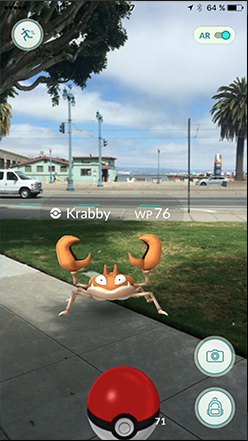
\includegraphics[width=.45\linewidth]{gfx/pokemon_go_gameplay}
        \caption{Screenshot of playing Pok\'{e}mon GO (reprinted from \url{http://www.pokemongo.com/de-de/explore/})}
        \label{fig:pokemonGOGameplay}
\end{figure}

\subsubsection{StreetConqAR}
StreetConqAR \citep{hock2014augmented} is a location-based augmented reality mobile exergame developed as an Android app. In the game, players have to conquer streets. The player that conquered most streets wins the game. To conquer a street, one has to walk to its street name sign and watch it through the smartphone. The app recognizes the sign and displays an augmented reality version of it with virtual colored letters blended above the original letters. To acquire the street, a riddle according to these letters has to be solved (see figure \ref{fig:streetConqARGameplay}).

As mentioned above, StreetConqAR presents a new way of creating anchors. Anchors are placed automatically based on real-world objects, the street name signs. The advantage of this approach is, that street name signs can be found all over the world, which means that StreetConqAR can be played all over the world, as well.

\begin{figure}[bth]
  \centering
        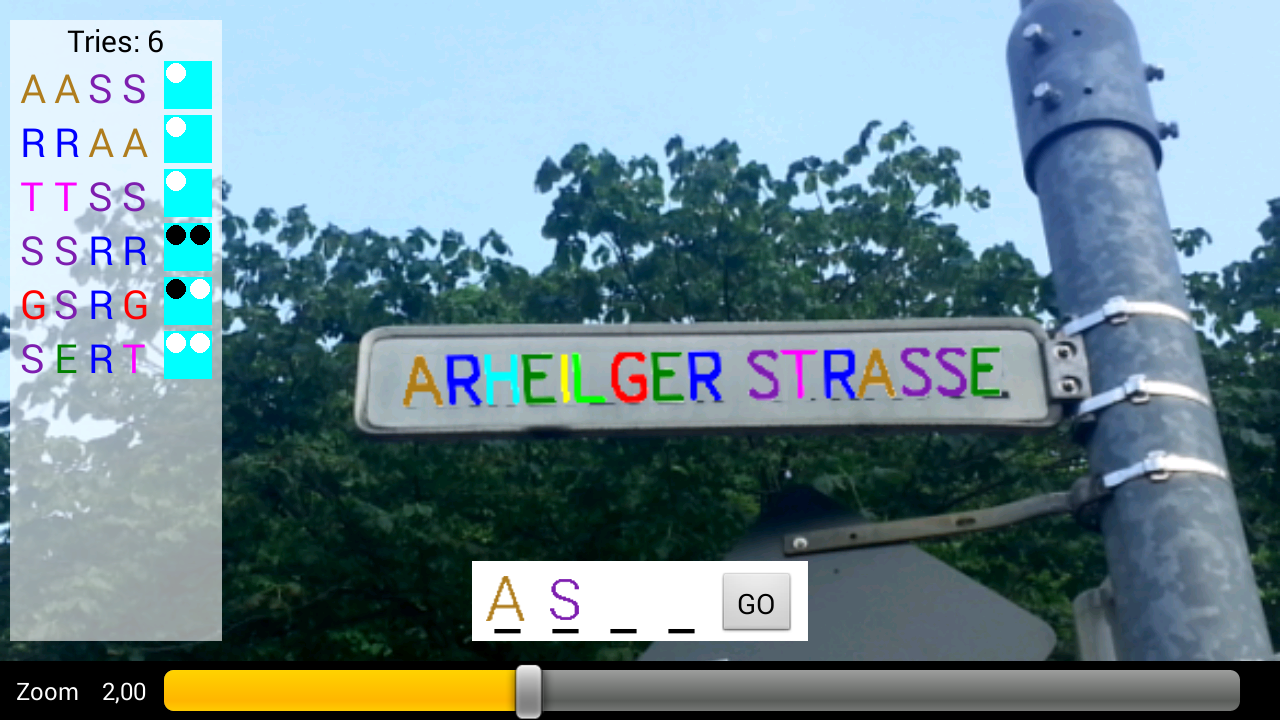
\includegraphics[width=.65\linewidth]{gfx/streetconqar_gameplay_reprint}
        \caption{Screenshot of playing StreetConqAR (reprinted from \citep{hock2014augmented})}
        \label{fig:streetConqARGameplay}
\end{figure}


\section{Vehicle Recognition}

\subsection{General}
Nowadays, vision-based recognition is a hot topic. Not possible to imagine automated manufacturing without it since many years, vision-based recognition became accessible for normal users with devices like the Microsoft Kinect \footnote{\url{https://developer.microsoft.com/en-us/windows/kinect}}, which is able to perform gesture recognition, for example. Another visual recognition which arrested attention (mainly because of privacy issues) in early 2015 was Facebook's face recognition system named DeepFace \footnote{\url{https://en.wikipedia.org/w/index.php?title=DeepFace&oldid=663499386}}, which searches photos, taken by Facebook users, for faces of other Facebook users.

Another field that is not so famous yet is the vehicle recognition. It is used in different systems like traffic monitoring and control or security and surveillance applications. Instead of a human observer sitting in front of some screens, an automated vehicle recognition system could do the task. Human constraints like multitasking and distinguishing among all the makes and models would be overcome by such a system.

Usually, the steps of a vehicle recognition algorithm are: (1) Feature Extraction, (2) Global Representation, and (3) Classification. Most of the systems do a preceding step and define a region of interest (RoI), which separates the vehicle from the background (see figure \ref{fig:vrSteps}).

\begin{figure}[bth]
  \centering
        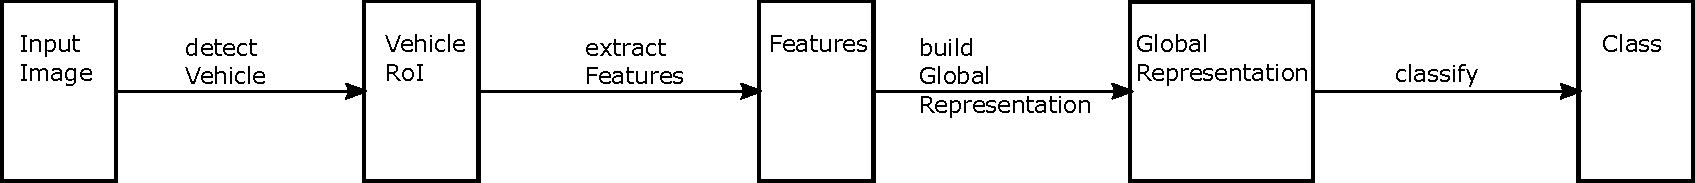
\includegraphics[width=.95\linewidth]{gfx/vr_steps}
        \caption{General steps of a vehicle recognition algorithm}
        \label{fig:vrSteps}
\end{figure}

Feature extraction in the vehicle recognition domain denotes identifying those parts of the image that are relevant (descriptive) for this class (type, make and/or model).

The global representation (or global descriptor) can be seen as the compound of all the relevant extracted features of one image. In simple phrase, the global representation describes a vehicle image of a specific class such that a classifier can understand it. The key task of building a global representation is making it informative and discriminating. There are many different ways to construct global representations, some of them are illustrated below.
Finally, the classification is the process of assigning a class (type, make and/or model) to a global representation of an unknown class.

There are different kinds of vehicle recognition, each for a different purpose and with its own challenges.

\subsection{Vehicle Type Recognition}
For an electronic toll collection system or for the analysis of traffic jams, the actual make or model of a vehicle is not relevant. Whereas the type of a vehicle helps to deduce the properties (like shape or weight) needed for such studies. So the Vehicle Type Recognition classifies vehicles into broad categories such as sedans, SUVs, trucks, vans, motorbikes, buses, etc. \citep{siddiqui2015robust}. This vehicle recognition is not described any further, since the next two recognition types are more akin to this thesis' topic.

\subsection{Vehicle Make Recognition}
Another way of classifying a vehicle is the Vehicle Make Recognition (or Vehicle Logo Recognition), which recognizes the make of a vehicle (like Mercedes, BMW, Porsche, etc.). This can either be done by solely using the vehicle's logo or by using its whole front or back.

To classify by the logo, an image matching with logo templates can be done \citep{jain2015car} \citep{wang2007fast}. For this, a set of vehicle logos is used as templates. Once the image snippet containing the logo has been detected, it is compared to each template using a template matching algorithm. The template with the highest match classifies the vehicle.

However, a more widely used technique is using feature detection with classification on the logo. \citeauthor{psyllos2010vehicle} use a database of logo images. During classification, each feature found inside the logo area of the queried image votes for each logo in the database, that contains a similar feature (evaluated by a Nearest Neighbor algorithm). The database logo with the most votes classifies the queried logo. There is one special thing about this approach, called \emph{Geometric Validation}. It means "that the coordinates of the keypoints (features) in the query and the matched database image are checked for geometrical consistency".

\citeauthor{rezaeivehicle} compared these two approaches with the result, that the image matching approach performed more accurate while a feature detection method was about 80\% faster \citep{rezaeivehicle}. While the logo detection alone as a preprocessing step of the recognition can be very time consuming \citep{siddiqui2015robust} and while this approach is very sensitive to occlusion due to the relatively small snippet of a vehicle image, using the whole front or back of a vehicle gives more robust classification results.

\subsection{Vehicle Make and Model Recognition}\label{sec:vmmrStateOfTheArt}
The most comprehensive kind of vehicle recognition and also one focus of this work is Vehicle Make and Model Recognition (VMMR), the identification of its make as well as its model (like Mercedes SL, BMW 3 Series, Porsche 911, etc.). For surveillance purposes, this recognition type extends the conventional number plate recognition. It can be used to double-check a recognized number with the corresponding make and model to fight the problem of false number plates. There are plenty of works referring to this topic and also some ready-to-use systems like Car-Rec \citep{jang2011car} or the \emph{VisualSearch} feature \footnote{\url{http://magazin.autoscout24.de/microsites/services/mobile/de-at/txt/android_txt3.html}} of the AutoScout24 app \footnote{\url{https://www.autoscout24.de/}}, which classifies vehicles by their backsides.
A surveillance and security application for static cameras is eyedea \footnote{\url{http://www.eyedea.cz/make-and-model-recognition/}}, that is able to recognize 500 vehicle models of the types bus, car, truck and van.

Most of the approaches use the front or the back side of the vehicle because it's the most descriptive part, usually containing the make's logo and, for the back side, even the lettering of the make and the model.

While most of the systems require strictly frontal or rear view images of vehicles, \citeauthor{shinozuka2013vehicle} proposed a solution to transform vehicle pictures taken from an angle of up to 60-degrees into pseudo frontal views.

The main differences among the various VMMR approaches are the construction of the global representations. Differences with minor importance are the choices of the local feature descriptor or the classifier, which does not mean that the local feature descriptor or the classifier have a minor effect to the classification performance, though.

\emph{"The quality of a global features representation technique is assessed by its processing speed, computational complexity in forming the holistic representations, and the VMMR accuracy which reflects its discriminative capacity in representing the different makes and models while generalizing over the multiplicity issues within a make-model class."} \citep{siddiqui2015robust}

\subsubsection{VMMR using Local Features Concatenation}
One classification approach is done by \citeauthor{petrovic2004analysis} \cite{petrovic2004analysis}, achieving recognition rates of over 93\%, tested on over 1000 images containing 77 different classes (make-models). The recognition is based on a relatively simple set of features extracted from frontal car images. A feature vector of predefined length (the \emph{global representation} as shown in figure \ref{fig:vrSteps}) represents one make-model. The global representation is just a pixel-wise concatenation of the vehicle's image. To determine the class of a queried vehicle, simple nearest neighbor classification is used among these feature vectors. The special thing about this approach is, that it uses only one vehicle image per make-model as training data. What is trained then, is the transformation of the training image into the global representation.

The features are not extracted from the whole vehicle image but from a RoI, a section inside of the image. This RoI is defined as an area around the car's number plate. Thus, relative to the number plate, the RoI is independent from the vehicle's actual location and scale inside the source image.

Starting with a straightforward representation by just concatenating the raw image values into the feature vector, \citeauthor{petrovic2004analysis} ended up with evaluating different sorts of image gradients. In figure \ref{fig:vmmrConcatenation}, examples of different global representations, created by different techniques, are listed.

\begin{figure}[bth]
  \centering
        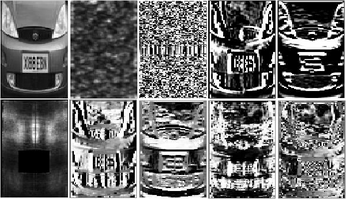
\includegraphics[width=.65\linewidth]{gfx/vmmr_concatenation_reprint}
        \caption{Examples of global representations (reprinted from \citep{petrovic2004analysis}): The first picture simply uses the source pixels. The other ones are based on the gradients of the image (with slightly different gradient transformations). The structure of the original image is still recognizable (more or less clearly) in the representation because of the concatenation of image pixels.}
        \label{fig:vmmrConcatenation}
\end{figure}

They also investigated in transforming the feature space via Principal Component Analysis (PCA) into a lower dimensional subspace to gain expressiveness and computation time. Finally though, tests including PCA performed slightly worse in most cases.

Another conclusion they made is, that a representation independent from color and contrast of the original vehicle image increases performance.

Pros of the approach of \citeauthor{petrovic2004analysis} are, that the recognition process is rather easy, which means, that it includes few steps and components for both, building the classifier and recognizing a new vehicle. Thus, it's easy to implement. It means also, that this process is easy to understand, because finding the nearest neighbor of a vehicle image in any kind of representation-space seems plausible to work properly.

There are also cons of their approach that will occur, when testing the system in real-life conditions. While the vehicle's global representation (its feature vector) is based on all of the pixels contained in its RoI, the recognition will not be robust to occlusion of some part of this area. For the same reason, slight changes in the camera's roll-angle or a displaced (or badly captured) number plate will also decrease the recognition performance. Hence, such an approach is not applicable in real-life scenarios.

\subsubsection{VMMR using a Bag-of-Words Model}
Another approach that tries to eliminate all the cons of the system proposed by \citeauthor{petrovic2004analysis} is made by \citeauthor{siddiqui2015robust} \citep{siddiqui2015robust}. Since that system is similar to the system proposed in this thesis, it will be discussed in more detail, here.

The challenges, \citep{siddiqui2015robust} attends to, are \emph{multiplicity} and \emph{inter-make and intra-make ambiguity}. \emph{Multiplicity} describes the problem of vehicles with different shapes or appearances all share the same name (make and model). An example for this is shown in figure \ref{fig:vmmrMultiplicity}.

While \emph{inter-make ambiguity} describes the issue of models from different companies being akin to each other, \emph{intra-make ambiguity} refers to different models from the same company that share similar features. Examples for this are shown in figures \ref{fig:vmmrAmbiguityInterMake} and \ref{fig:vmmrAmbiguityIntraMake}, respectively.

\begin{figure}[bth]
  \centering
        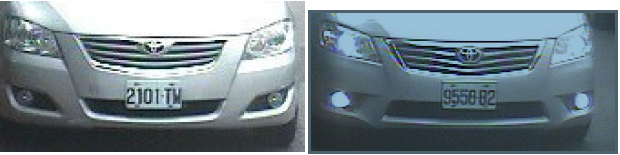
\includegraphics[width=.75\linewidth]{gfx/multiplicity_reprint}
        \caption{Multiplicity issue. Both pictures show a Toyota Camry, from 2008 and 2010, respectively (reprinted from \citep{siddiqui2015robust}).}
        \label{fig:vmmrMultiplicity}
\end{figure}
\begin{figure}[bth]
  \centering
        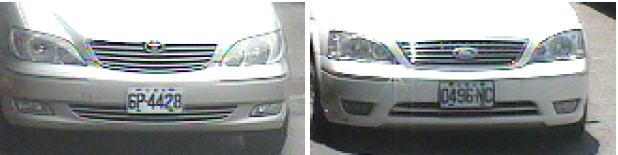
\includegraphics[width=.75\linewidth]{gfx/ambiguity_intermake_reprint}
        \caption{Inter-make ambiguity issue between a Toyota Camry and a Ford Mondeo (reprinted from \citep{siddiqui2015robust}).}
        \label{fig:vmmrAmbiguityInterMake}
\end{figure}
\begin{figure}[bth]
  \centering
        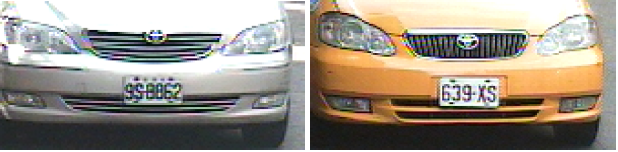
\includegraphics[width=.75\linewidth]{gfx/ambiguity_intramake_reprint}
        \caption{Intra-make ambiguity issue between a Toyota Camry and a Toyota Altis (reprinted from \citep{siddiqui2015robust}).}
        \label{fig:vmmrAmbiguityIntraMake}
\end{figure}

So the task is to build a global representation, "that accounts for intra-class differences and inter-class similarities, thereby solving the multiplicity and ambiguity issues in VMMR" \citep{siddiqui2015robust} and that is robust to occlusions and small changes in the camera angle.

In contrast to the approach of \citeauthor{petrovic2004analysis}, the global representations of this system are constructed using a bag-of-words model instead of concatenating the pixel values of the RoI. With a bag-of-words model, data is represented by occurrences of distinct codewords, while the codewords are collected in a dictionary (the bag). This means, similar to the Vehicle Make Recognition system proposed by \citep{yu2013vehicle}, mentioned above, the global representation is a histogram. Each bin of this histogram represents one distinct feature-codeword while the height of the bin indicates the occurrence-frequency of this specific feature-codeword in the source image.

The set of all feature-codewords, the \emph{visual words}, build the dictionary or \emph{bag}. A feature-codeword in this context is not a feature but a representative of several similar features. This way, the size of the dictionary does not only control the size of the global representation (number of bins in the histogram) but also the threshold, at which several features are clustered into one single dictionary feature-codeword. So the dictionary represents the essence of the key features (in this case SURF \citep{bay2008speeded}) of all the training images.

\paragraph{Dictionary Generation}\label{par:dictionaryGenerationStateOfTheArt}
Two different schemes of dictionary generation are proposed by \citeauthor{siddiqui2015robust}. One called \emph{Single Dictionary} (SD), the other called \emph{Modular Dictionary} (MD). For the SD, all the local features of all training images are clustered. Each cluster center then represents one codeword of the Single Dictionary. The number of clusters defines the size of the dictionary, therefore. An advantage of this scheme is, that considering the combined set of features over all the training images (across multiplicity and ambiguity) strengthens the discriminability of this dictionary. A disadvantage is, though, that one cluster could contain features that are similar but originate from different make-model classes. To cope with this, a dictionary is only built out of the training images for one specific make-model class (in the same way as described above), resulting in one dictionary per make-model class. The set of all the codewords of those dictionaries form the MD. An advantage, besides the one noted above, is the flexibility when adding new training data. Only the dictionary of the specific class has to be rebuilt, which saves processing time. A disadvantage is the increased size of the Modular Dictionary compared to the Single Dictionary. Although the size of one of its per-class dictionaries can be smaller than that of the Single Dictionary, multiplying this with the number of make-model classes will boost the number of overall codewords. For an illustration of the two schemes, see figure \ref{fig:dictionarySDMD}.

\begin{figure}[bth]
  \centering
        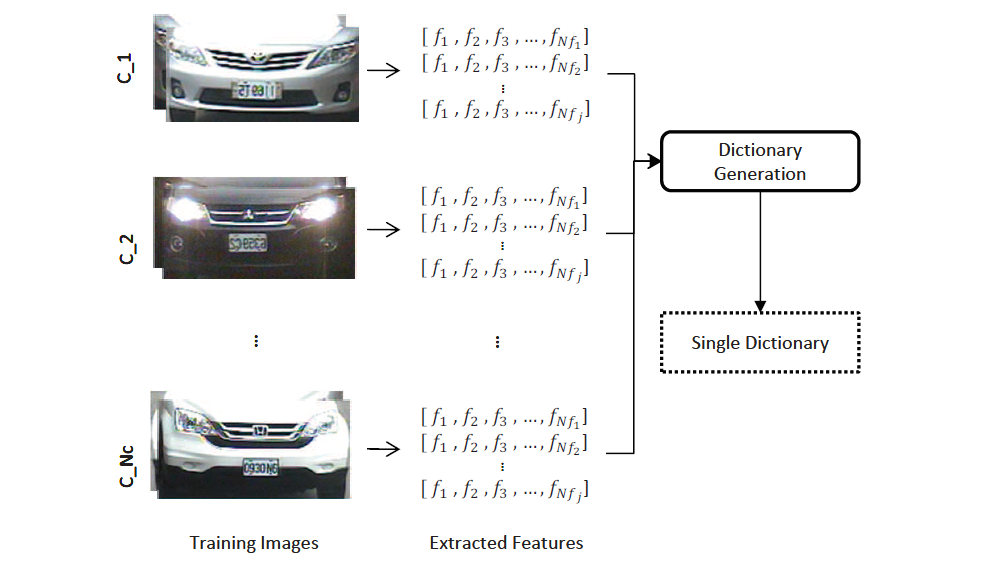
\includegraphics[width=.95\linewidth]{gfx/single_dictionary_reprint}
        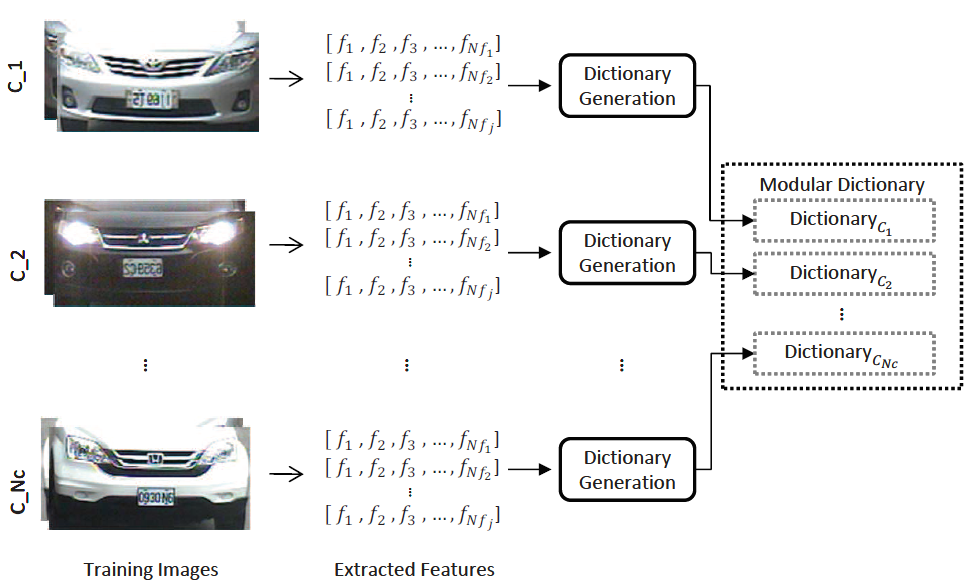
\includegraphics[width=.95\linewidth]{gfx/modular_dictionary_reprint}
        \caption{Dictionary building schemes. Above for the Single Dictionary, below for the MD, where $f_n$ is the $n$-th feature of one image of the respective class $c_m$, $N_c = $ number of classes, and $Nf_j = $ number of features of the $j$-th image of a respective class (reprinted from \citep{siddiqui2015robust}).}
        \label{fig:dictionarySDMD}
\end{figure}

\paragraph{Results}
For the classification (the last step of the vehicle recognition process from figure \ref{fig:vrSteps}), a multi-class SVM-based classifier is used. The classifier is trained to learn both similarities among different generations of the same make-model class and differences among inter-class models.

Experiments of \citep{siddiqui2015robust} showed that the SD, contrary to the expectations, slightly outperforms the MD. On the other hand, the dictionary training time is much less for the MD. However, for an application, where the dictionary is built offline and does not need to be updated (or only seldomly) during runtime, the Single Dictionary is the better choice, according to this experiments.

%TODO \section{Number Plate Region Detection}

%\subsection{Definition}
%In contrast to "Number Plate Detection" or automatic license plate recognition (ALPR), where (also) the content of the number plate is desired.

%TODO: Reference already working Systems. I heard that automatic recognition is used in Österreich to recognize the Vignette.

%TODO: Refer to [7] and [8], [9], [10]

%TODO: Explain Hough Transform in detail with image and formula and such (as Hock did in Technical Basics)







%*****************************************************************************
%*****************************************************************************
\chapter{Concept}\label{ch:concept}
%*****************************************************************************
%*****************************************************************************
This chapter is about a new way of automatic content generation for exergames. It presents an approach to use real-world vehicles as anchors. Using vehicles as anchors means recognizing their make and model and integrating its virtual counterpart via AR into the game play.

In the first section, the basic concepts needed for a location-based exergame and what makes such a game popular are discussed. Later on, the design of \emph{RacecAR GO}, a location-based exergame that implements this concept, is presented. In the subsequent section, the prototype of RacecAR GO, that will be implemented along with this thesis, is described.

As VMMR is an important part of this game, an approach for this is proposed in the final section of this chapter.


\section{Location-based Exergame using AR}
This section is about the preparation and evaluation of the basic concepts to build a location-based exergame. It first discusses the type and how to integrate anchors, then it generally evaluates the properties of such games that motivate people to play and to move. Later, the usage of augmented reality as a technology to improve the user experience is discussed. A list of requests for a location-based exergame as a result of this evaluation is presented in the final section.

\subsection{Anchors}\label{sec:anchorsConcept}
As a reminder, \emph{"anchors in pervasive [...] games are well defined positions, where reality and virtuality are blurred"} \citep{hock2014augmented}. An exergame that shall be playable all over the world also requires anchors placed all over the world.

In chapter \ref{sec:anchorsStateOfTheArt}, many approaches for creating anchors have been proposed with pros and cons. It turned out that designer placed anchors are usually well-placed and well-fitted to the game's purpose, but include an expensive design process. As a result, games with designer placed anchors mostly provide content for only a few limited regions.

On the other hand, placement of anchors by the users takes the work out of the designer's hands and provides the possibility to create content all over the world. As a drawback, the quality of such anchors usually suffers and depends on the goodness of the editor and on the user's design-skills. Another disadvantage is, that the user must pass the design-phase before he is able to play the game. Such an approach is not suited for a game that smoothly integrates into the player's everyday life and shall every time be playable without any pre-setup.

The automatic anchor generation offers a good middle course for this request, as it doesn't include an expensive design process but nevertheless produces well-placed anchors depending on the creation rule.

\subsubsection{Natural Anchors}
\citeauthor{hock2014augmented} proved in his thesis, that placing anchors at street name signs creates a game that provides content for many regions (urban and rural ones) all over the world \cite{hock2014augmented}. Additionally, he not only used the positions of the street name signs but also included the object itself as an anchor into the game. This comes with some ambiguity issues, because the term anchor is used for both, the location and the related object.

As a solution, this thesis introduces a new term, the \emph{natural anchor}, which is an object, that exists in both, the real world and the game world. At its position, the reality intersects with the virtuality.

This means, that the real object and the virtual object are semantically the same. \citep{hock2014augmented}'s game \emph{StreetConqAR}, a street name sign in reality is also a street name sign in the virtual game world. In contrast to that, anchors in Ingress or Pok\'{e}mon GO are often placed at distinct objects like monuments or landmarks, though, but in the game world, the semantic meaning of these objects is different. They turn into portals for Ingress and into Pok\'{e}Stops or gyms for Pok\'{e}mon GO.

This thesis proposes to use real-world vehicles as natural anchors for an exergame. The way these are integrated into the gameplay and a discussion about the characteristics of this special type of anchor can be found in chapter \ref{sec:usageOfAnchors}.

\subsection{The Art of Motivating People to do Something for their Health}\label{sec:motivationToMove}
In the previous chapter, many different examples of exergames have been listed, each having its own approach to motivate its players to do something positive for their health. The key seems to be to encourage the players by something that is fun. This something's main intention is not doing sports. The health aspect is just a side-effect of playing the game.

In the following, the concepts used by various exergames to motivate their players to move are compared and discussed.

An often used motivation is to achieve (virtual) property. It seems that players keep on playing a game as long as there are achievements of some kind to accumulate their (virtual) property. This concept is used by Pok\'{e}mon GO, for example, where the property is the personal Pok\'{e}dex with the captured Pok\'{e}mon. It is also used by Ingress where the property are the hacked portals. Additionally, the player could form an emotional relation to its property, which also keeps him on playing.

Another concept, akin to achieving property, is the achievement of reputation. The more and the harder a player trains, the more reputation he can get inside the game. This is used in StreetConqAR by giving the players titles as "King of ..." or "Lord of ...", in Ingress by gaining experience points or in Pok\'{e}mon GO by becoming a Pok\'{e}mon master.

In the exergame \emph{The Running Dead}, proposed in the beginning of this thesis, a simple but strong motivation to run is used: Fear. Fear of what will happen if a zombie catches me.

A motivation that is deeply anchored into the human's roots is based on the hunter-gatherer principle.

\subsubsection{Hunter-Gatherer Principle}
Long time ago, when our civilization was young, most of the people were hunter-gatherers. This means, people spent a big part of their lives with hunting for animals or gathering fruits to eat or items to construct tools of. For such a civilization, these things were necessary to survive. After some time, people became farmers and the number of hunter-gatherers decreased.

Today, most people aren't hunter-gatherers (nor are they farmers). But although our everyday life differentiates so much from that of a hunter-gatherer, a desire for this kind of life still seems to be lurking in many of us. Why else would there be millions of people playing Pok\'{e}mon GO, in which the main task is to hunt and to gather little monsters?

\subsection{Augmented Reality}
As discussed in the State of the Art chapter, augmented reality is an up-and-coming technology used in many application fields. Utilized in a pervasive game, it can help the player to immerse into the game. But using AR as a fancy technology for its own sake isn't the right way to design a good game. It's better to focus on a lasting and catching gameplay and using AR to support this instead of trying to impress the player with stunning technology \citep{wetzel2008guidelines}.

\subsection{Requirements}
To create a successful exergame that motivates its players to do something for their health, following requirements (\emph{GR} for game request) can be deduced from the previously said:
\begin{itemize}
  \item\textbf{GR1:} The game has to be playable everywhere at anytime
  \item\textbf{GR2:} The players must be able to start a game session without needing any previous setup
  \item\textbf{GR3:} The game uses a principle to motivate players to move
  \item\textbf{GR4:} The game integrates augmented reality in a reasonable and supporting manner
\end{itemize}
\emph{GR1} contains two aspects of the game. The first one relates to the game's platform and the needed hardware. To be playable everywhere, the game should run on a mobile device. The second aspect is the game content (the anchors), that has to be available everywhere a player could have the idea to go for a quick session.


\section{Concept of RacecAR GO}
\begin{figure}[bth]
  \centering
        
\includegraphics[width=.25\linewidth]{gfx/app_icon}
\end{figure}

In this section, the concept of the game \emph{RacecAR GO}, that uses real-world vehicles as anchors, is presented. It shows approaches to fulfill the previously declared \emph{GRs} and also discusses challenges that accompany them.

\subsection{Overview}
RacecAR GO is a location-based exergame. It's played outside on a mobile device. The player's task is to find and capture vehicles by taking a photo of them with the device's camera. The virtual counterpart of each captured vehicle is then stored in the player's virtual garage. At certain locations, players can compete against each other to win other player's cars or to lose the own ones.

Not only is the name RacecAR GO akin to Pok\'{e}mon GO, also the gameplay is. This is because Pok\'{e}mon GO motivated millions of people to play and to move, so its concept can be regarded as exemplary.

\subsection{Platform}
RacecAR GO is realized as a client-server app. The client app is available for both, iOS and Android. The advantage of current devices running iOS or Android is, that they usually come with a camera, a GPS sensor and mobile internet. The server stores and manages all user data and attends to the recognition of the make and the model of a captured car (for an illustration with some exemplary tasks see figure \ref{fig:platform}).

\begin{figure}[bth]
  \centering
        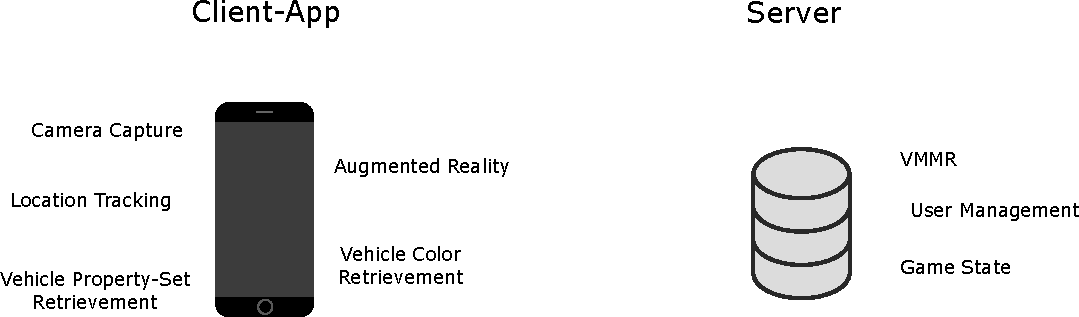
\includegraphics[width=.95\linewidth]{gfx/platform}
        \caption{Used platforms with tasks}
        \label{fig:platform}
\end{figure}

\subsection{Gameplay}\label{sec:gameplay}
The gameplay is described on the basis of the storyboard in figure \ref{fig:storyboard}. Each subsection inside this section refers to one of the storyboard's views. A player starts the game by creating an account or by being automatically logged in with his existing account.
The game has a centralized structure, i. e. each view is accessed via the menu. With a \emph{Back} button, the user can always return view by view back to the menu. The menu has six entries, each representing one area of the app:
\begin{itemize}
  \item\textbf{Capturing:} To capture new vehicles
  \item\textbf{Garage:} Shows all captured vehicles with its properties. Vehicles can also be upgraded here
  \item\textbf{Map:} Shows a map displaying nearby car dealers or playgrounds
  \item\textbf{Car Dealer:} To sell captured cars to
  \item\textbf{Playground:} To compete with other players
  \item\textbf{Settings:} Shows the game settings
\end{itemize}
The user is able to achieve money during play, so his current credit is always displayed at the top bar of the game. This is for a motivational reason, because the player earns money by physically moving with a speed less than seven km/h. So always displaying the current credit will motivate him to walk farther and watch it increasing.

\begin{figure}[btph]
  \centering
        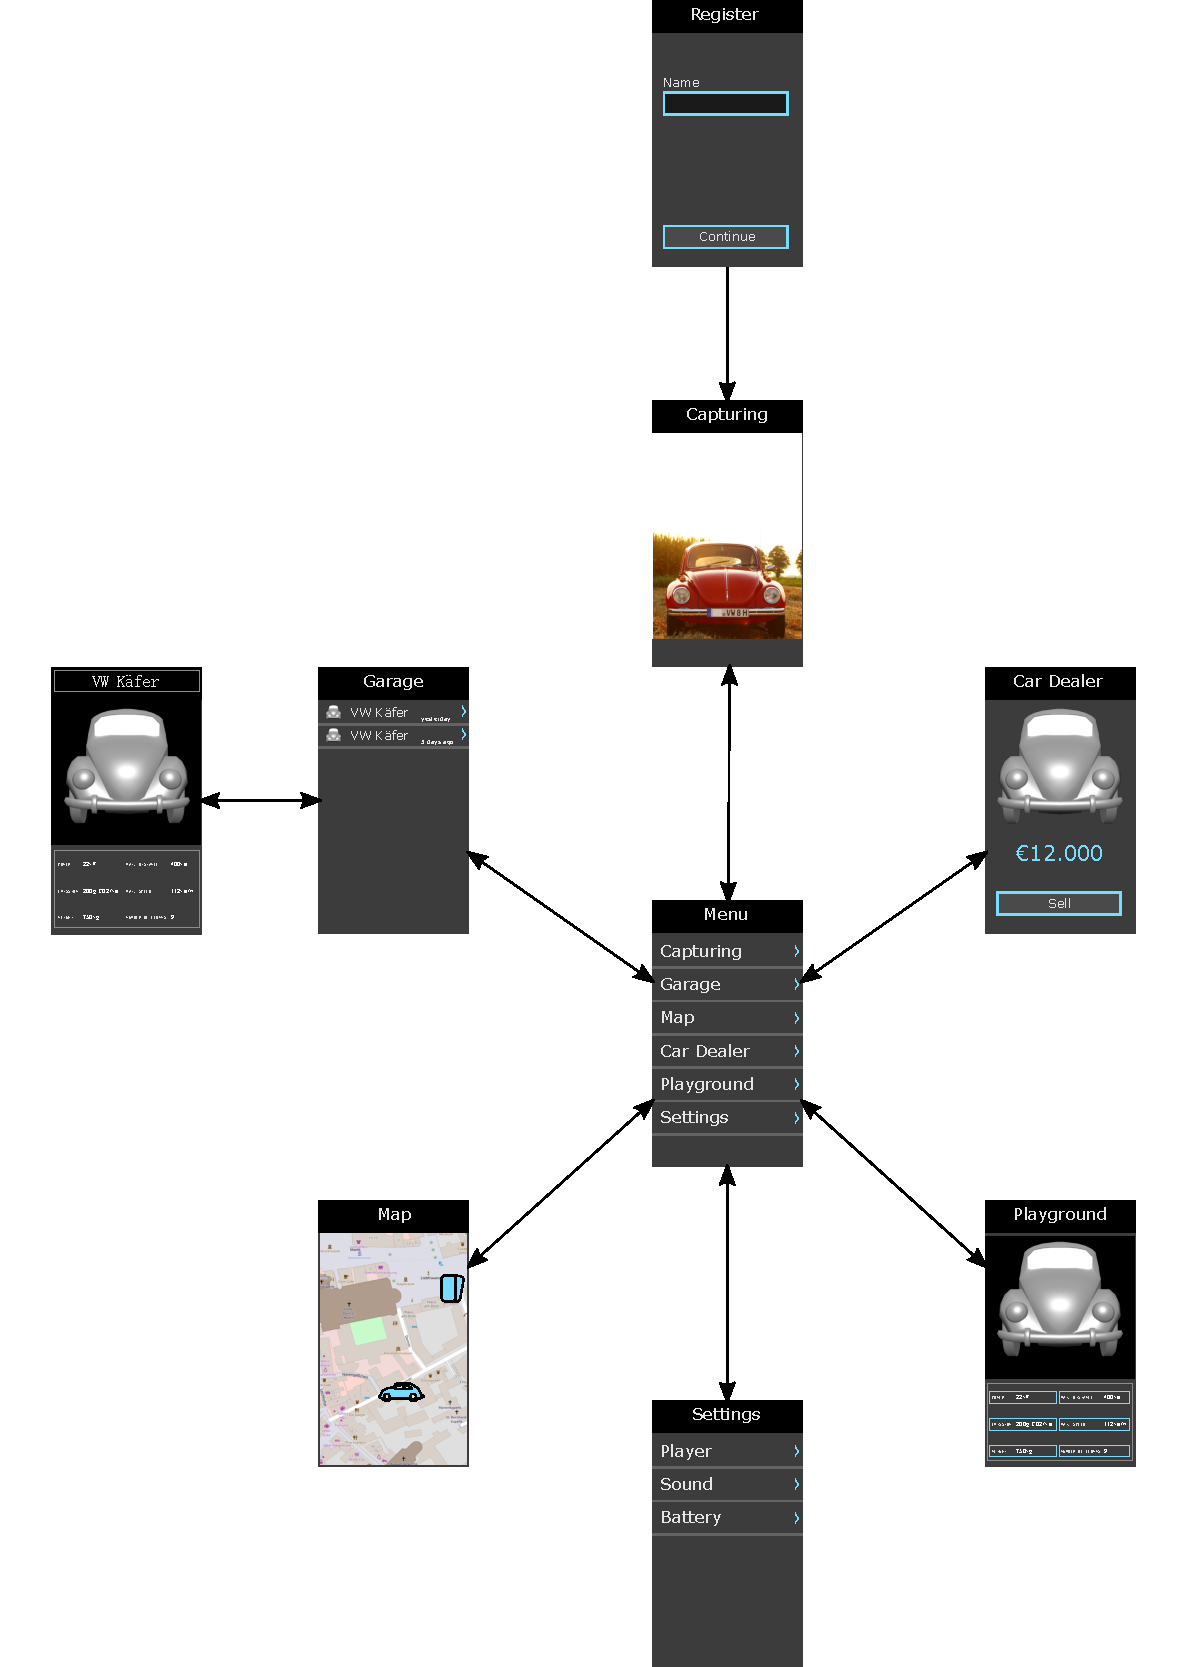
\includegraphics[width=.8\linewidth]{gfx/storyboard}
        \caption{Storyboard of RacecAR GO: In the \emph{Map}-view, the vehicle icon marks a car dealer, whereas the play cards mark a playground.}
        \label{fig:storyboard}
\end{figure}

\subsubsection{Capturing}
At the start of the game, the player finds himself directly in the \emph{Capturing} view, ready to capture new vehicles for his garage. This fulfills \emph{GR2} which demands that the player must be able to play without any annoying setup. This view is also accessible via the menu. The capturing process is divided into four steps and is illustrated in figure \ref{fig:capturing}.

\begin{figure}[btph]
  \centering
        \includegraphics[width=.75\linewidth]{gfx/capturing}
        \caption{Capturing Process of RacecAR GO}
        \label{fig:capturing}
\end{figure}

\begin{enumerate}
  \item As long as the capturing process is in step 1, the device shows the vehicle as the camera takes it. To capture it, the player has to point the device's camera towards the desired vehicle's front view or back view. In the background, the app sends a picture of the vehicle to the server. The picture has to be the front view or the back view, because along with the picture, the hashed number plate is sent to the server. This is to check, if the user hasn't captured the car yet. If he has, he cannot capture it for a second time.

Otherwise, the server performs a VMMR (see chapter \ref{sec:vmmrConcept}) and sends the retrieved make and model along with its respective properties (in the example a "VW K\"afer" with a matching property-set) back to the client.
  \item Step 2: With the received make and model, the app chooses the correct virtual vehicle with that make and model and blends it above the real vehicle (see chapter \ref{sec:usageOfAR} for details). Additionally, it retrieves the vehicle's color from the captured image. This isn't a straightforward task, as there are multiple colors with multiple shadings occurring on a vehicle. One approach is to retrieve the color class containing the most pixels and choose the most similar color from the manufacturer's list of varnishes for that vehicle.

The player is then able to walk around the real vehicle while he only sees the colored virtual one through the device. He can interact with the vehicle by touching on the door or on the hood to open and close it. To continue, the player has two options. He can either touch the trash icon and abort the capturing, or he can opt for the garage icon, to park the vehicle in his garage.
  \item To park the vehicle in his garage, the player first has to fulfill a small task in step 3. For the task, a vehicle part appears that matches to the captured vehicle. This part could be a door, a steering wheel, a car seat, an engine or another part the captured vehicle consists of. In the example, it's an engine. This part overlaps the vehicle and is fixed to the device's screen, such that when the player moves around the vehicle, the part overlaps different areas of it. The player's task is to place this part at the correct position. E. g. for the engine and the VW K\"afer (which has a rear engine), the user would have to walk around the car, touch on the engine cover to open it, place the engine at the correct position (by moving the device such that the engine icon overlaps the position where the engine of the real car would be) and finally touch the wrench icon.
  \item If the placement is correct, the vehicle will be parked in the player's garage. If not, the capturing will be aborted. The vehicle is stored along with its property-set, containing its power, weight, emission, etc. This data is retrieved from an API like \emph{CarQuery} \footnote{\url{http://www.carqueryapi.com/}}. In most cases, it's ambiguous to deduce the property-set from a vehicle's picture, as the appearance of the vehicle doesn't change (or only marginally) for different engine configurations. For this reason, the server would have to search clues in the picture, like the exhaust or additional letters on the backside or the grill of the car that indicate a distinct configuration.
\end{enumerate}

\subsubsection{Garage}
The captured vehicle is then parked in the player's garage. The garage can only be accessed via the menu. It lists all the vehicles, the player has already captured. Touching one vehicle item opens the vehicle's details. Inside the details, the vehicle's properties as well as its 3D-model are shown. If there's a small arrow behind a property, it means that the player has enough money to afford an upgrade for that property. Touching the arrow performs the upgrade and pays the money from the user's credit.

\subsubsection{Map}
The map shows the surroundings of the player. Its purpose is to visualize the location of nearby car dealers and playgrounds. Locations of car dealers are marked with a vehicle symbol, playgrounds are marked with playing cards. The player is always in the center of the map.

\subsubsection{Car Dealer}
This view is, like the playground, only available, if the player is physically near to a car dealer marked in the map. Here, he can sell his captured cars. This might be useful for frequent cars, as the player should usually have plenty of them in his garage. Nonetheless, the dealer pays a much better price for rare cars.

\subsubsection{Playground}
When I was a schoolchild, me and my friends played a card game every morning in the school bus. Where I come from, this game is called \emph{Supertrumpf} or \emph{Autoquartett}. Internationally, it's also known as \emph{Top Trumps}. A card set relates to one theme, mostly cars. A card displays a car of a specific make and model, along with its property set, mostly including the number of cylinders, the maximum speed and the engine power (see figure \ref{fig:playcard} for an example). Each player gets the same number of cards in the beginning of the game and has to stack them, such that he (and no one else) cannot see another card than the topmost one. The player left to the giver starts to meld a property with the associated value of his topmost card. The other players announce the respective value of their card in turn. The player with the best property-value wins that round and receives all topmost cards, which he has to put at the bottom of his card stack. The winner also melds for the next round. If there's a draw, all players with the same property-value play a further round with their next card. The winner then receives the cards of both rounds. The game ends, if one player has won all of the cards.

For RacecAR GO, Supertrumpf will be adapted to be played at the playground locations. Entering such a location, the player has the possibility to start or to join a game with other players at that location. The own card stack will be represented by the vehicles in his garage. During the game, the app displays a virtual play card as the top of the stack. Melding a property is done by touching the respective field on the virtual card. A message after each round informs each player who has won that round. Losing a virtual card also means losing the respective vehicle out of the garage. Winning cards of other players also means that the respective vehicles (including possible upgraded properties) are added to the winner's garage. A player can leave the game whenever he likes to. He necessarily leaves the game as soon as his card stack (and so his garage) is empty. A game necessarily ends, if one player has gained the vehicles of all other players.

RacecAR GO uses the following vehicle properties to list on a play card:
\begin{itemize}
  \item\textbf{Engine Power:} A conventionally used property in Supertrumpf.
  \item\textbf{Maximum Speed:} Also a conventionally used property in Supertrumpf.
  \item\textbf{Weight:} The weight of the vehicle. An important performance measure, often neglected in this kind of games, although an increasing engine power that comes along with an increasing weight doesn't necessarily improve a vehicle.
  \item\textbf{Maximum Distance:} The maximum distance, the vehicle is expected to reach with a full fuel tank (or battery). This property has been added, because there are not only petrol heads playing the game but also people thinking of vehicles as means of transport. This kind of people are rather interested in practical measures of a vehicle than in performance measures.
  \item\textbf{Emission:} The emission of vehicles is a hot topic nowadays. Never having seen this property on any card when I was a child, today's people should a fortiori be aware of the emissions produced by a car. This does not mean that the author of this thesis generally doesn't like vehicles with high emissions. It's rather about the conscious usage of such.

Additionally, vehicles that would have lost any competition in a Supertrumpf game in my childhood will beat reputed super sports cars in this domain.
  \item\textbf{Number of Clowns:} Denotes the number of clowns, that fit into the vehicle.
\end{itemize}
\begin{figure}[btph]
  \centering
        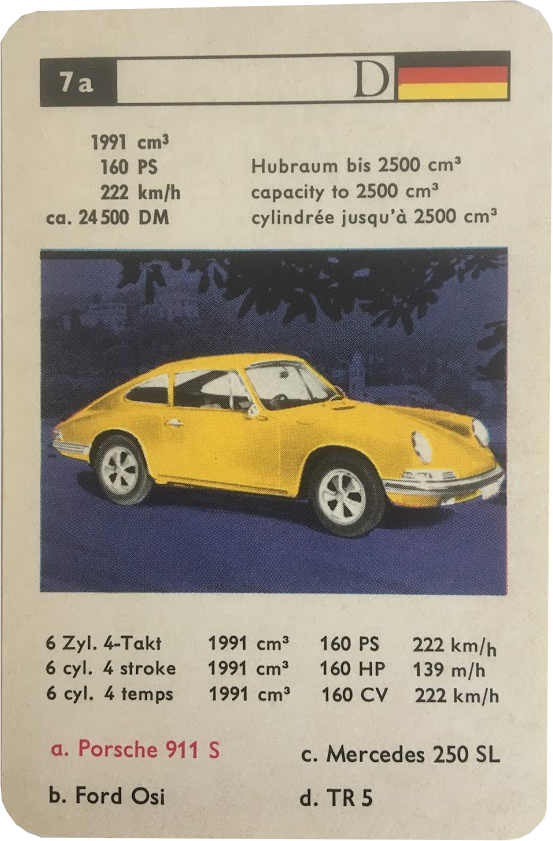
\includegraphics[width=.25\linewidth]{gfx/playcard}
        \caption{Example of a play card showing the first generation of the Porsche 911. It is part of the card game \emph{Sportwagen Quartett Nr. 52522}, published by \emph{F. X. Schmid Vereinigte M\"unchener Spielkarten Fabriken KG}.}
        \label{fig:playcard}
\end{figure}

\paragraph{Expectations}
Players could be motivated to visit the playground locations with the prospect of winning rare and upgraded vehicles with little effort. Additionally, players will have to upgrade their vehicles to succeed in the game. As a result, players are motivated to walk by feet, as the game rewards this with virtual money, which is needed to upgrade a property.

On the other hand, players could regard Supertrumpf as unfair and could get demotivated after playing, because a vehicle, including much effort to capture and much money to upgrade, can easily be lost to another player. Concurrently, opponent's rare vehicles can be won the same way. The game's evaluation has to show, if the hurdle for a player to use the playground is too high to clear. If so, a preceding step could be included, in which the player decides which vehicles of his garage shall be put onto the card stack and which ones should be left secure in his garage. This would lower the hurdle to play.

\subsubsection{Settings}
In the settings, the player is able to change his password and to enter the battery saving mode (as in Pok\'{e}mon GO) which turns off the screen if it is not directed towards the user. This is necessary because an app with these requirements will consume much battery power. The durability of the battery would otherwise be a killjoy for motivating the player to move and to immerse into the game.

\subsection{Usage of Anchors}\label{sec:usageOfAnchors}
This section is about the types of anchors that are used by RacecAR GO and about their implications. As described in section \ref{sec:gameplay}, the game content includes three different location-based items that serve as an anchor: Vehicles, car dealers and playgrounds (actually there are four, as the user can be regarded as a natural anchor itself, since he is integrated into the game as himself, at least in the map view).

In the following, the choice of the anchor for each of these items is discussed.

\paragraph{Vehicle Anchors}
In the game, vehicles function as natural anchors. This means objects, that exist in both, the real world and the virtual world. The big advantage of such anchors is, that they do not have to be distributed a priori by a designer, they are already there.

A special characteristic of the vehicle as anchor is, that it tends to be not fixed in its location. This breaks the criterion of an anchor as a "well-defined position" \citep{hock2014augmented}. But since the vehicle as natural anchor does only persist during the capturing process, where its location is fixed (hopefully, but see section \ref{sec:hazards} for hazards), this fact hasn't any impact on the gameplay.

A positive effect of using vehicles is, that urban areas become attractive to walk in. As \citeauthor{gehl2013cities} states, today's cities are car-friendly and unwalkable \citep{gehl2013cities}. People usually don't find it very attractive to do sports there, like jogging or cycling. From the perspective of this game, these are good prerequisites to play at. Being on the prowl for seldom vehicles, a car-friendly and unwalkable environment turns into a paradise.

In contrast to the anchors placed in Ingress or Pok\'{e}mon GO, the actual distribution of the vehicle anchors cannot be controlled by the game. The distribution changed continuously and cannot be tracked as a whole. For the capturing process, only the local distribution is important. Considering the map showing the number of vehicles per capita for regions in the whole world (see figure \ref{fig:worldVehicles}), there are only a few regions, where it could be difficult for a player to find enough vehicles to have fun playing this game (e. g. in Central Africa or in parts of Asia). So the predefined \emph{GR1}, that the game has to be playable everywhere at anytime, is fulfilled by the vehicle anchors.

\begin{figure}[btph]
  \centering
        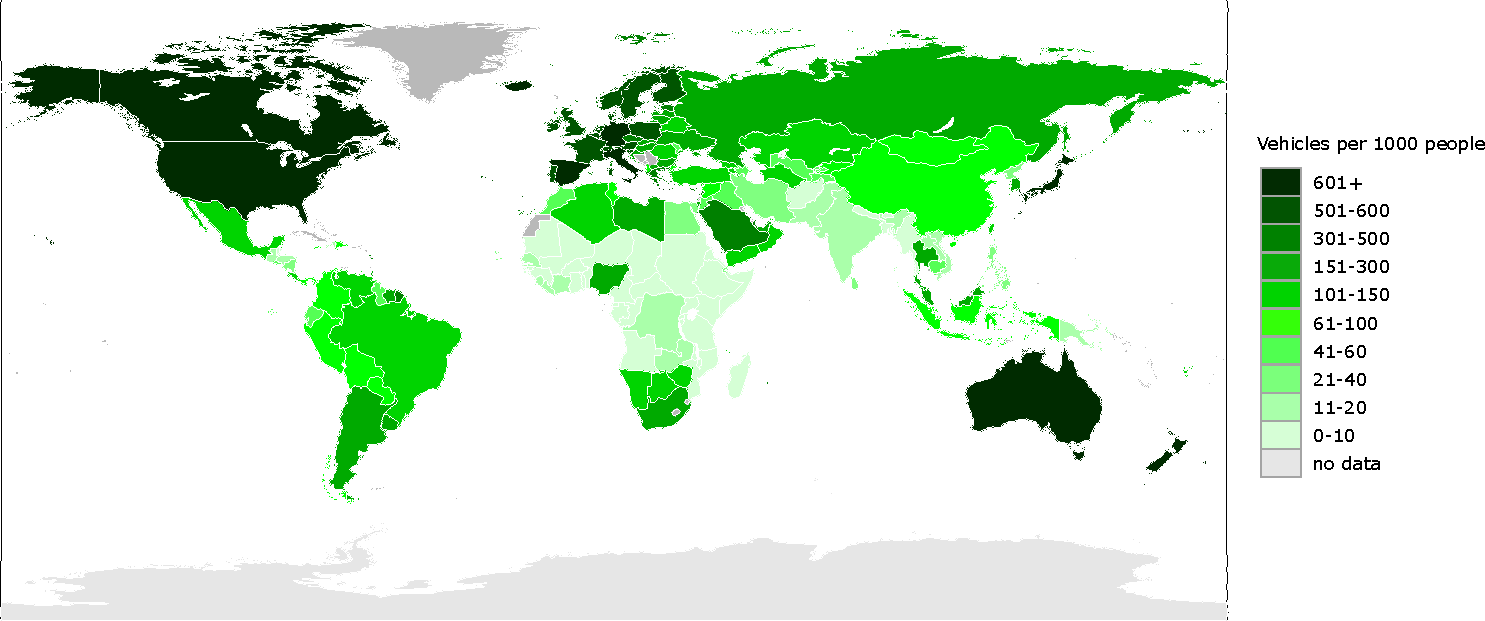
\includegraphics[width=.95\linewidth]{gfx/world_vehicles_per_capita}
        \caption{World vehicles per capita (reprinted from \footnote{\url{https://commons.wikimedia.org/w/index.php?title=File:World_vehicles_per_capita.svg&oldid=242848798}})}
        \label{fig:worldVehicles}
\end{figure}

There are also some drawbacks, though. The real-world part of the natural anchor does not have to be distributed, indeed, but the virtual part, the counterpart of each real-world vehicle, has to be created a priori. The VMMR machine has to be trained for each make-model as well. A solution to this problem is to only cover a limited amount of make-models. These include the most-frequent ones, like the VW Golf, which exists nearly all over the world, but also a few rare models. With such a starter-set, the game can be played everywhere, whereas only a subset of the cars around the player can be captured. A crowd-based approach to extend this starter-set is possible. If a player tries to capture a vehicle, that is not yet supported by the app, he would be asked to specify the make and the model. The VMMR machine could then use this data to train itself. The missing virtual vehicle counterparts could also be submitted by a crowd. As it is done for Ingress, there should be a reviewer to check the user-created content.

\paragraph{Car Dealer Anchors}
Car dealers are also represented by natural anchors. This means, that car dealers in the game are also car dealers in the real-world. The location of car dealers can be retrieved from Google Maps. The advantage of using this type of anchor is the semantically sensible inclusion of car dealers into the game. It's safe to assume that the distribution of car dealers in the world is well-suited to the game's needs. Where there are cars, there have to be car dealers. If there's a region that lacks car dealers, the game can still be played, as selling captured cars is not essential for the gameplay.

\paragraph{Playground Anchors}
As opposed to this, playgrounds are an essential part of the gameplay, without which all the hunting and gathering would be aimless. For this reason, well-distributed anchors are needed. Whereas most vehicles need gas to drive, gas stations can be considered as well enough distributed, such that most players are able to visit one without much effort.

\subsection{Usage of Augmented Reality}\label{sec:usageOfAR}
As denoted in the gameplay, augmented reality is used inside this app to blend the virtual vehicle above the real vehicle during the capturing process. It is expected that the way of blending the real and the virtual world - by the transformation of a real car over an augmented car into a virtual car - greatly improves the immersion effect for the player (\emph{GR4}).

The task is to blend the virtual vehicle in a way above the real vehicle, such that both objects overlap perfectly and the player is able to walk around the vehicle to regard it from different views. To solve this task, there are multiple approaches, which are discussed in the following.

\paragraph{Square Markers}
As described in chapter \ref{sec:augmentedRealityStateOfTheArt}, square markers are very efficient to track, even for mobile devices. Using square markers for the vehicle capturing process would implicate that there have to be square marker pictures being placed on the real-world vehicle, which isn't the case.

\paragraph{Number Plate as Marker}
This approach uses the vehicle's number plate as the AR marker. The marker tracking is realized with NFT (see chapter \ref{sec:augmentedRealityStateOfTheArt}). During the capturing process, the number plate of the vehicle gets detected. When the camera moves, the tracked features from the number plate are used to calculate the location and pose of the vehicle.

ARToolKit provides an implementation for this for mobile devices. The realtime-calculation of the location and pose of the vehicle from its number plate performed quite well, producing robust results for blending the virtual vehicle above the real one (although this only works for perspectives, where the number plate is visible, i. e. not for the vehicle's side view). But the initial tracking of the number plate's features took up to a minute (for a number plate width of 100px on an Intel(R) Xeon(R) CPU E3-1230 V2 @3.30GHz of the year 2012). This is because the process has been designed to train the feature recognizer in an offline phase and just use it in the online phase without changing the set of known features. Since the number plate of the captured car is not known in the offline phase and since the player doesn't want to wait one minute until the AR magic begins, this technique is not applicable.

\paragraph{EURO-Badge as Marker}
In most European countries, a number plate contains a euro badge (see figure \ref{fig:euroBadge}). In contrast to the number plate, features of the euro badge can be tracked in the offline phase, because the badge is the same on each number plate.
Tests with ARToolKit on a mobile device resulted in an improper calculation of the location and pose of the badge, which was perhaps down to the fact that there aren't enough (unambiguous) features to track inside this badge image.

\begin{figure}[btph]
  \centering
        
\includegraphics[width=.25\linewidth]{gfx/marker_full}
        \caption{Euro badge of a European number plate (here from Germany)}
        \label{fig:euroBadge}
\end{figure}

\paragraph{Model-based Tracking}
As described in chapter \ref{sec:augmentedRealityStateOfTheArt}, this approach relies on a 3D CAD model as reference to identify features in the captured image. Based on the reference model, its pose inside the captured image can be deduced from any perspective. Since the 3D CAD models are already present (the virtual vehicle models), this approach is very suitable to fulfill the requested task.

\paragraph{Smartphone Motion Sensors}
Another option to blend the virtual vehicle appropriately above the real one is to use the mobile device's motion sensors. In contrast to the aforementioned methods, this one is not vision-based. To initially fix the virtual vehicle to the real one, the position of the number plate is used. From that time on, the motion of the device is appropriately applied to the virtual object such that the player can move and rotate the device while the virtual object is fixed above the real vehicle.

This approach works well in tests, although the virtual object and the real object sometimes drift apart over time. This is because the virtual object is only once (in the beginning) stitched to the real vehicle. After that, accumulating errors in the device motion updates could account for the drift.

\subsubsection{Conclusion}
Only the model-based tracking is able to fulfill all the requested tasks accurate enough. Only here, the user would be able to walk around the real car while the virtual car model is always overlaying it correctly. Nevertheless, it is assumed that this technique has high hardware requirements, because features in the camera image have to be tracked and matched with the reference model in realtime.

\subsection{Privacy Concerns}
As mentioned before, a vehicle has to be photographed to be captured. Even more, its number plate (in hashed form) will be stored on the server. But is the personality right of the owner violated by this procedure? In Germany, the main field of application for the app, it's generally granted to publish a photo of a vehicle showing the vehicle's number plate \footnote{\url{https://www.rechtambild.de/2014/09/fotografieren-und-veroeffentlichen-von-autokennzeichen-was-ist-erlaubt/}}. The publishing of the number plate does not violate the personality right of the owner, because civilians usually cannot deduce the owner from a number plate. Nevertheless, there's no definitive right for this and it will be decided from case to case.

Because the app does not publish the number plate but only stores a hashed version of it, there should be no problem with this. But to be on the safe side, place a hint in the app to urge the players to forbear capturing a vehicle, if the owner is present and does not give his permission.

\subsection{Hazards}\label{sec:hazards}
Pok\'{e}mon GO proved, that games that are played outside can cause hazardous moments for the players and their environment. That there’s even a website, the \emph{Pok\'{e}mon GO Death Tracker} \citep{PokemonGoDeathTracker}, shows the severity of this issue.

Due to the affinity of RacecAR GO with Pok\'{e}mon GO, it is obvious that it also has the potential to cause hazardous moments. Because the gameplay inevitably takes place at locations that are made for vehicles, players will often move inside potential danger zones. Hence, they always need to be aware of being attentive to that. It is also possible that he game causes an inappropriate behavior. Players running onto the street to capture a rare vehicle parked over there, people invading private grounds to photograph a vehicle parked in the entry or hindering driving cars to capture them are only a few possibilities of unwanted behavior of RacecAR GO players.

The choice of using gas stations as playgrounds also involves dangers. At gas stations, there is usually a lot of traffic. Crowds of people standing there and playing RacecAR GO could for one thing cause a jam and for another thing endanger themselves when carelessly standing in the way of driving cars.

To react to this, RacecAR GO will show a hint on startup to inform the player of always being attentive when playing the game in city traffic and to not disturb or invade other people’s privacy. Wether the players themselves feel unsafe while playing the game has to be evaluated during the evaluation (see chapter \ref{ch:evaluation}).

\subsection{Cheating}
Like Pok\'{e}mon GO, RacecAR GO will implement an algorithm to check, if a player is walking by feet or if he is moving with a car. He will only be rewarded for walking by feet. For a walked distance, he will earn money to tune his cars, although there is no deeper relation between walking by feet and earning money. Nor is there a deeper relation in walking by feet and brooding Pok\'{e}mon eggs.

Another check to prevent users from cheating is to store the hash of the number plate of a captured vehicle to hinder the player to capture the same vehicle multiple times (see chapter \ref{sec:gameplay}).

To capture a vehicle, a player could simply google for a picture of it and photograph this one instead of walking through the city and doing it the hard way. Since common mobile phones do not have a depth camera installed, there's no solution for this, yet.

\subsection{Classification as a Location-based Exergame}
In the previous chapter, exergames have been defined as video games, that combine healthcare exercises with gameplay fun, whereas the healthcare aspect is not primarily focused. To succeed in the game, however, physical activity is necessary.

RacecAR GO fulfills these criteria. To succeed in the game, players have to physically move to vehicles, car dealers or playgrounds, which are location-based. The primary focus of the gameplay is the hunting and gathering, though. This is also the motivational principle (\emph{GR3}), that is used by the game. Another principle to motivate the players to move is the achievement of (virtual) money when walking by feet.

The game also covers concepts of pervasive games, such as breaking the magic circle in a spatial and temporal manner. As a result, it integrates smoothly into the player's everyday life: Players would be encouraged to walk through their environment with eyes open to discover a vehicle that is desired for the game.


\section{Concept for a RacecAR GO Prototype}
Along with this thesis, RacecAR GO will be implemented prototypically. To match the timeframe of a master thesis, a reasonable subset of features will be defined in the following.

\subsection{Limited Story}
The prototype focuses on the hunting and gathering of vehicles. The upgrading and selling of vehicles as well as the playground has been omitted (whereas the vehicles in the garage are displayed as play cards with corresponding properties). Without these features, a map would be useless, so it has been omitted, too. See figure \ref{fig:storyboardPrototype} for the covered views and components.

\begin{figure}[btph]
  \centering
        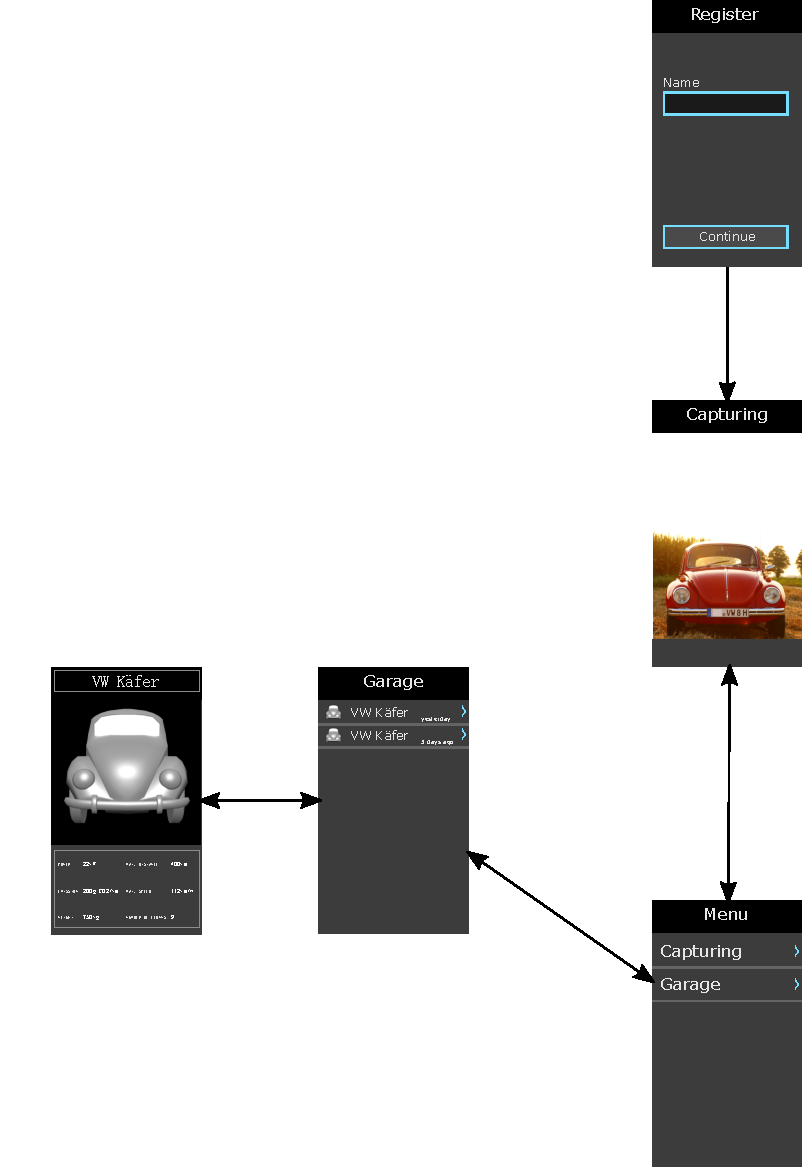
\includegraphics[width=.6\linewidth]{gfx/storyboard_limited}
        \caption{Storyboard of the RacecAR GO prototype: Only the capturing process will be implemented within the prototype.}
        \label{fig:storyboardPrototype}
\end{figure}

\subsection{Platform}
The prototype will only be implemented for iOS, especially for iPhones. The implementation excludes the iPad, because the game requires a mobile device, that the player always carries with him and that is compact enough to walk through the city with. It's possible to play RacecAR GO on the iPad, however, but to experience a smooth integration of the game into the everyday life, the iPhone is the better choice.

\subsection{Vehicles}
The type of vehicles that shall be capturable in RacecAR GO can be of an arbitrary kind, from motorbikes over racecars to trucks. A limitation for the prototype is, that only passenger cars are covered by the app. This is due to the fact, that the VMMR machine, that will be implemented along with this thesis, recognizes vehicles solely based on their front. More precisely, a specific region around the vehicle's number plate is chosen to classify the vehicle with. As motorbikes don't have a wide front and in most cases don't even have a number plate, they are not covered by the prototype. The problem with trucks (or buses) is, that the region around the number plate of a truck is not descriptive enough to differentiate it from other trucks of a different make and model (for further reading see the drawbacks in chapter \ref{sec:regionAroundNumberPlate} or refer to the ambiguity issues in the bag-of-words section of chapter \ref{sec:vmmrStateOfTheArt}).

As described above, the app comes with a starter-set of vehicles, that can be recognized and captured. For the prototype, this set is limited to 10 different vehicles. See chapter \ref{sec:supportedVehicleClassesImpl} for an explanation, which make-models have been chosen and why. Unlike to the full version of the app, there is no possibility to add further make-models but for the game designer to add them manually.

\subsection{Vehicle Capturing}\label{sec:vehicleCapturingProto}
There are also some restrictions that have to be done for the capturing process (see figure \ref{fig:capturingLimited}). As said above, a specific region around the number plate is sent to the server for VMMR. To find the number plate in the captured image, a watermark showing a number plate's frame is blended above the camera image. For best recognition results, the user has to position his iPhone such that the watermark covers the number plate of the real car in location, orientation and size. In contrast to the full version, the prototype does not automatically send the captured image to the server. The player has to touch the gearbox button to start the capturing process. Because the prototype-server doesn't perform a hashed-number-plate-check, if the user already captured this car, the number plate will be blacked out in the transferred image for privacy concerns.

The server answers the VMMR request solely with the make and model of the car. For each covered make-model, the client stores one corresponding property-set, that is automatically applied to the respective captured vehicle.

After having received the make and model, the client loads the respective virtual model and blends it in AR manner above the real car (as it is done for the full version of RacecAR GO). The color of the vehicle will not be tracked, so a blank virtual model is used. The following mini-game of placing a vehicle-part at the correct location is omitted for the prototype, though it is still possible to move the iPhone and see the virtual model still overlaying the real vehicle adequately. Touching the garage-symbol will immediately store the captured vehicle into the garage and thus finish the capturing process.

%TODO: Auch hier die Schritte in der Grafik nummerieren
\begin{figure}[btph]
  \centering
        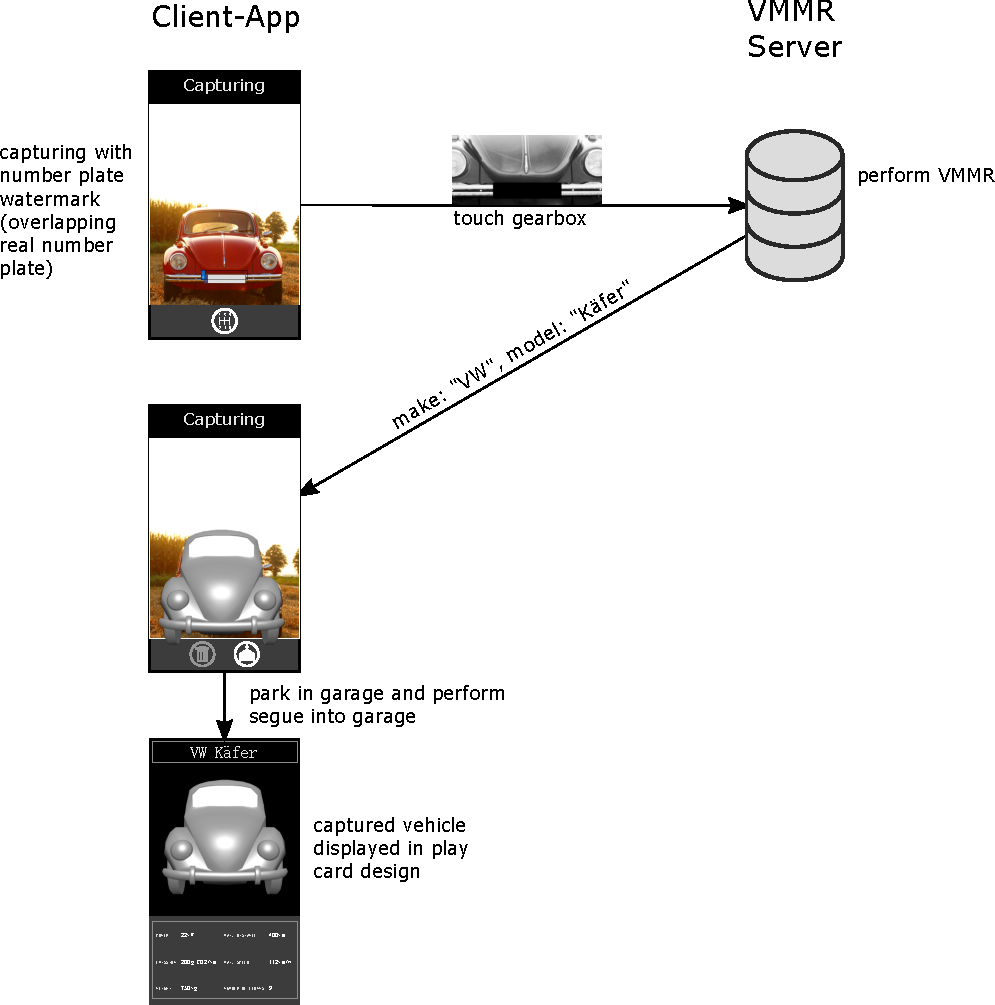
\includegraphics[width=.75\linewidth]{gfx/capturing_limited}
        \caption{Capturing process of the RacecAR GO prototype}
        \label{fig:capturingLimited}
\end{figure}

\subsection{Augmented Reality}
Because the recognition of the vehicle is fixed to its front and since the capturing task with fitting the vehicle parts will not be implemented, it's sufficient to overlay the real vehicle with the virtual one in the front view.

For this, three of the aforementioned approaches come into question. First one would be to use the vehicle's number plate as AR marker. As mentioned above, the test results of tracking the marker and calculating its pose and location were quite well whereas the initial setup of this marker took too long for a reasonable user experience.

Another approach is the model-based tracking, which was proposed to be used for the full version of the app, because it is able to calculate the vehicle's pose and location from arbitrary perspectives.

The last approach is to use the smartphone's motion sensors to deduce the vehicle's pose and location.

Both, the second and the third approach are applicable to the task. Because of the expectedly high computational resources needed for the model-based tracking on a mobile device, the third one will be implemented.


%=============================================================================
\section{Concept of Vehicle Make and Model Recognition}\label{sec:vmmrConcept}
%=============================================================================
In this chapter, the VMMR system that is used in \emph{RacecAR GO} will be presented. Until now, the work on vehicle recognition has mainly been dedicated to the subject of security observation of parking spaces, toll stops, country borders, etc. In this thesis, the domain of application is something different, using it in a mobile game and capturing the vehicle images with a mobile phone's camera. One main challenge to handle when recognizing vehicle makes and models is to fight ambiguity and multiplicity issues.

\subsection{Excursion to the Ambiguity and Multiplicity Challenge}\label{sec:excursionAmbiguity}
As stated by \citep{siddiqui2015robust}, the assembled recognition model should cope with ambiguity and multiplicity issues. Multiplicity means the problem of cars with different appearances but with the same make and model, whereas the ambiguity describes the challenge to differentiate between similar vehicles that do not have the same make (inter-class ambiguity) and/or model (intra-class ambiguity), though.

Assuming a player of RacecAR GO walks along the street and suddenly, he spots a Porsche 911 parked beside him. Fortunately, in front of the Porsche, there's enough clearance to take a photo of its front. Already imagining himself watching this beautiful and seldom car in his virtual garage, wouldn't it be annoying if the app would classify this Porsche 911 as a rather ordinary Mini One, just because of the similarity between the shape of their headlights (see figure \ref{fig:ambiguityPorsche})? Such a failure could kill all the motivation of a player to continue playing, and thus losing the healthy benefits of this game. As a result, the game would miss its purpose to motivate people to move.

\begin{figure}[btph]
  \centering
        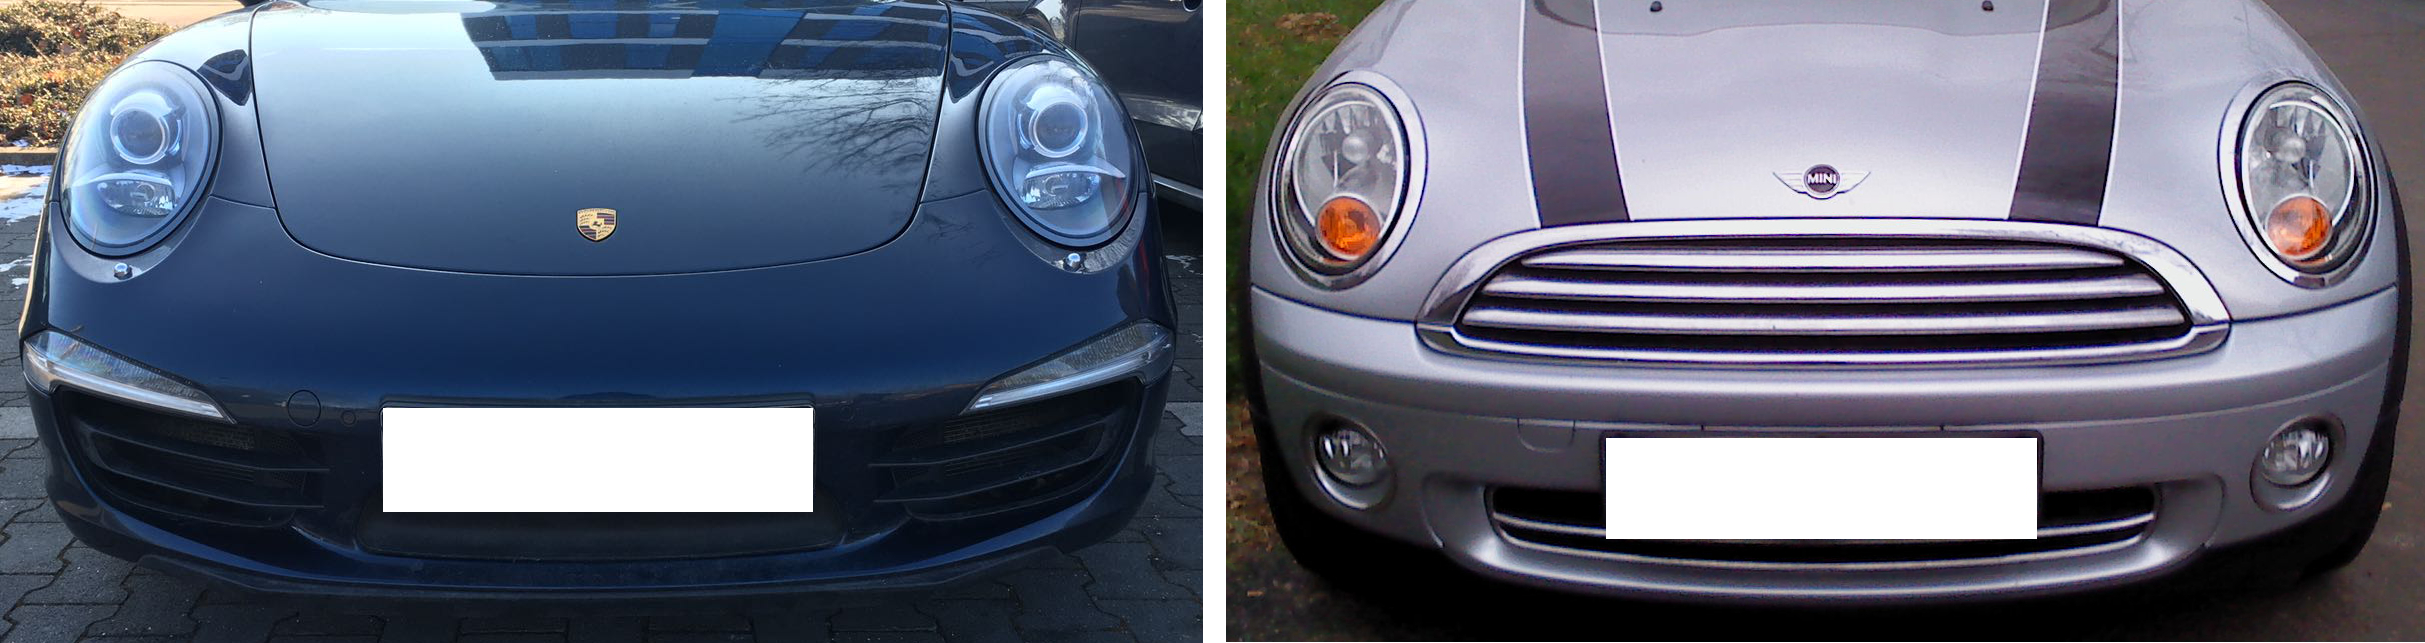
\includegraphics[width=.75\linewidth]{gfx/ambiguity_porsche_911_mini}
        \caption{Ambiguity (inter-class) issue between a Porsche 911 (991) and a Mini One (R55)}
        \label{fig:ambiguityPorsche}
\end{figure}
Additional to the inter-make ambiguity issues mentioned before (also those in chapter \ref{sec:vmmrStateOfTheArt}), there's the problem of rebadging because of licence products. In most cases, these vehicles differ solely in the logo on the hood and on the back (see figure \ref{fig:ambiguityRebadging}).

\begin{figure}[btph]
  \centering
        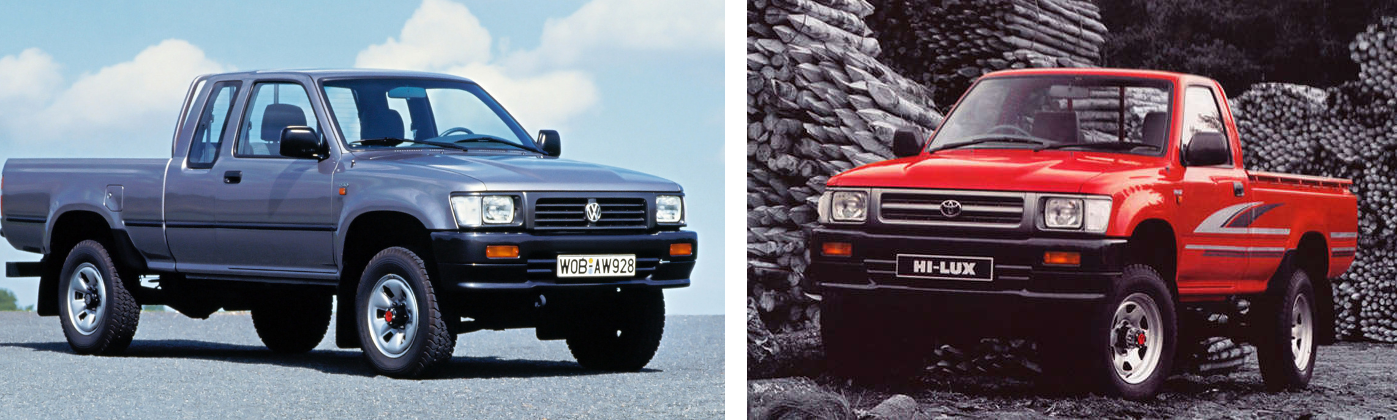
\includegraphics[width=.75\linewidth]{gfx/ambiguity_rebadging}
        \caption{Ambiguity (inter-class) issue as the Volkswagen Taro \footnote{\url{https://img.favcars.com/volkswagen/taro/volkswagen_taro_1994_images_2.jpg}} is a rebadged Toyota Hilux \footnote{\url{http://image.priceprice.k-img.com/ph/images/article/1020/hilux-5th.jpg}}}
        \label{fig:ambiguityRebadging}
\end{figure}

\subsection{Overview}
From the use cases of this game, some requirements for the VMMR system (\emph{VR} for VMMR request) can be deduced:
\begin{itemize}
  \item\textbf{VR1:} Robustness to partial occlusion: In reality, there is rarely enough clearance around a parked car to take a photo of it without another object occluding a part of it. The other object might be a bush, a tree, a street light, another car, etc. So if the recognition system cannot cope with a photo of a partially occluded vehicle, the player might be irritated while looking for a vehicle with enough clearance around it and might lose fun to continue playing.
  \item\textbf{VR2:} Robustness to different camera roll-angles: As the input image does not come from a fixed camera but from a smartphone's camera held by a person, it cannot be ensured that the smartphone is always horizontally aligned with the photographed car's horizontal axis.
  \item\textbf{VR3:} Robustness to different lighting conditions: There's the legend of a project of the US Army trying to recognize partially hidden tanks in the woods. So they trained a neural net with pictures of woods with tanks behind trees and pictures of the same woods without tanks. The result was impressive as the net recognized images that hadn't been used for training. After that, the researchers took more pictures of the same woods, but the net failed to discriminate between the two classes. Finally, it turned out, that the pictures with tanks in it were taken on a cloudy day, while those without tanks were taken on a sunny day. \emph{"The net had learned to recognize and generalize the difference between a woods with and without shadows!"} \citep{dreyfus1992artificial}. To be able to play the game in the daytime as well as at night-time, the recognition system has to be independent from the lighting conditions of the photographed vehicles.
  \item\textbf{VR4:} Ability to cope with ambiguity and multiplicity issues: Mentioned above, the proposed system must be able to differentiate between similar vehicles of different make or model (ambiguity) and not to differentiate between vehicles of the same make and model but with a different appearance (e. g. due to different generations of the model) (multiplicity).
\end{itemize}
The bag-of-words model implicates some advantages in contrast to the local features concatenation approach by \citeauthor{petrovic2004analysis}. Because the global representation is not directly depending on the pixels-grid of the source image, it is robust to occlusion to some extent. As long as the remaining set of local features is descriptive enough, the vehicle can still be classified. Another advantage is the robustness to slight changes in the camera's roll-angle or in the perspective. Depending on the local descriptors (\citeauthor{siddiqui2015robust} used SURF, which is rotation invariant), rotated local features would still result in the same bag-of-words histogram.

A downside of this approach is, though, that the local features lose their spatial information on their way into the global representation. The original position of a local feature is neither encoded inside of the local feature descriptor nor inside of the global descriptor. So an image with same features which are in a different order gets the same match. Nevertheless, the recognition system in RacecAR GO will take advantage of the bag-of-words model, meeting requirements \emph{VR1} and \emph{VR2}.

To gain independence from lighting conditions (\emph{VR3}) - and thus to avoid training a classifier that can solely tell the difference between pictures taken in the morning and pictures taken at noon - three things are done. The first thing is populating the training set with multiple images per make-model class, whereas the per-class-images are taken at different times of day by different kinds of weather (see chapter \ref{sec:datasetCreation}). The second thing is the preprocessing of each vehicle image. Lighting information will be subtracted out of an image before it enters the recognition system (see chapter \ref{sec:roiExtraction}). Third thing is the usage of local feature descriptors, each of which is invariant to illumination changes.

To fight the multiplicity issues, as demanded by requirement \emph{VR4}, models of different generations are trained into different classes. To handle the ambiguity challenges, the classification process will be optimized (see chapter \ref{sec:parameterTuning}) and due to the small number of realized makes and models for the RacecAR GO prototype, these can be well-chosen to minimize ambiguity and multiplicity problems (see chapter \ref{sec:choiceOfVehicleClasses}).

\subsection{VMMR Workflow}
At this point, after the requirements for the system are defined, its components and their interaction will be described as the \emph{VMMR workflow}. An illustration for this is shown in figure \ref{fig:vmmrWorkflow}.

\begin{figure}[btph]
  \centering
        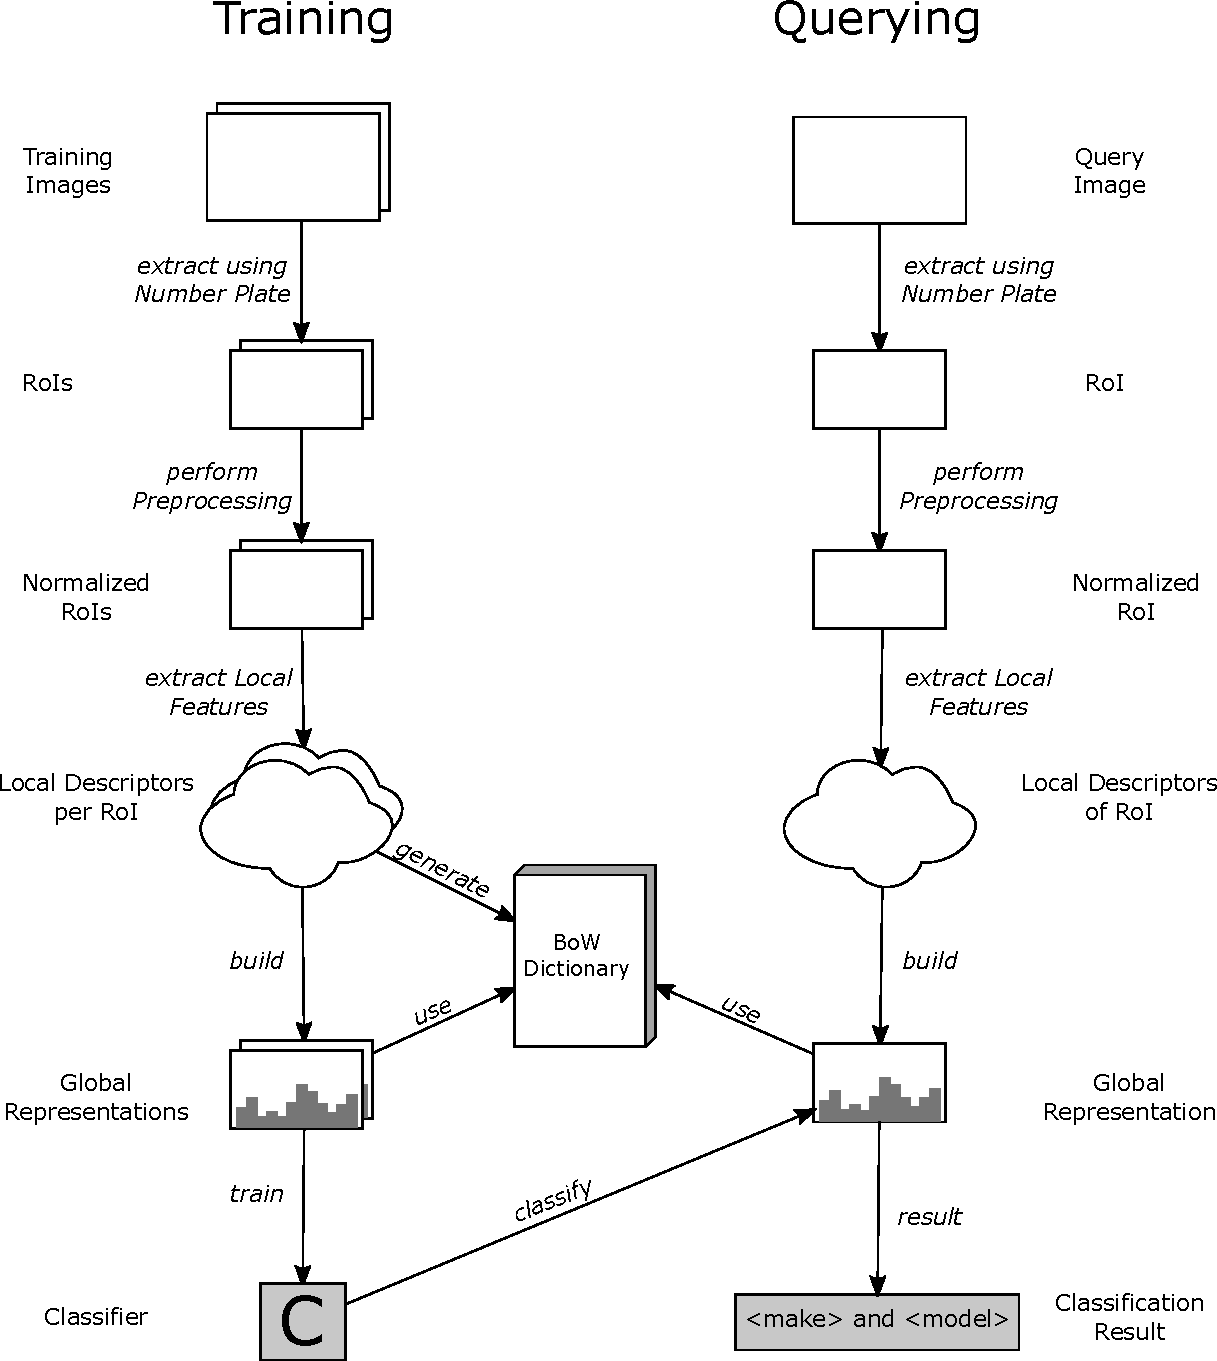
\includegraphics[width=.75\linewidth]{gfx/vmmr_workflow}
        \caption{VMMR workflow as it is used in the RacecAR GO prototype}
        \label{fig:vmmrWorkflow}
\end{figure}
%TODO: Workflow figure: Show kaefer photos for query AND? train. Show blue circles as descriptors

Actually, there are two workflows. One to train the system (the \emph{Training}-workflow), the other one to use the system to classify an image of unknown make and model (\emph{Querying}-workflow).

The query-workflow basically consists of the same steps listed for a vehicle recognition in figure \ref{fig:vrSteps}, with the preceding step of a RoI-extraction. Both workflows start with extracting the RoI from the input image. The RoI contains a descriptive part of the vehicle illustrated in the image (see chapter \ref{sec:roiExtraction} for details about the RoI extraction). After that, the RoI is used to search for local features. In the training-workflow, the local features from all RoIs of all makes and models from the training data are used to build the bag-of-words dictionary. With this dictionary, the local features of a specific make-model RoI are converted into a histogram, the global representation of this make-model-instance. In the training-workflow, the make-model of the global representation is known. In the query-workflow, it's not.
During training, a classifier is trained by all these global representations with their corresponding make-models. Whereas in the query-workflow, the trained classifier will be used to get a corresponding make-model for a global representation.

The single steps of the workflows will be explained in more detail in the subsequent sections and are oriented by the approach presented by \citep{siddiqui2015robust}.

\subsection{RoI Extraction}\label{sec:roiExtraction}
As mentioned as the optional preceding basic step for a general vehicle recognition (see figure \ref{fig:vrSteps}), detecting and extracting a region of interest (RoI) is part of most vehicle recognition algorithms. The input of this step is the raw image of a vehicle, e. g. taken with a smartphone camera.

The task of the RoI-extraction is to separate the foreground from the background. So the output of this step is a smaller part of the inputted image, containing just the vehicle, where, in the optimal case, all information not belonging to that vehicle has been erased.

The advantage of using a RoI instead of the whole input image in the following workflow steps are, that for one thing, the global representation of the vehicle is solely built out of information exclusively containing descriptive vehicle data. Simultaneously, all the noise caused by the background will disappear. All this increases the expressiveness of the global representation. For another thing, the processing speed increases due to the lesser amount of pixels compared to the original image.

\subsubsection{Preprocessing}
There is usually some preprocessing done on the RoI. The target is to transfer the different RoIs into a state of reasonable comparability. This is often called the \emph{normalization} of the RoI. So one preprocessing step is the normalization of its size. The term \emph{size} of the RoI is ambigue here. It can either describe the number of pixels in each dimension, the RoI is made of. Or it means the size of the cutting out of the original image. Only before normalizing the size (former one), these two are equal. To avoid misunderstandings, the latter will be referred to as the \emph{extent} of the RoI.

Both, the size and the extent of the RoI, need to be adjusted for each single vehicle image. The extent, because the original vehicle photos all have different dimensions and have been taken with different distances from the vehicle. So the extents vary from image to image to cover always the same amount of vehicle information. Hence the sizes of the resulting RoIs are also different. For the recognition, especially for the search of local features, it is necessary that all the RoIs are equal in size. So they are all scaled to a constant size (for concretely used sizes and extents, see table \ref{table:tunedParameters}). If not, a local feature found in a RoI of small size would not be found in a larger RoI, although a vehicle of the same make and model is depicted.

Another preprocessing step is the normalization of color and contrast. In \emph{VR3}, the urge for independence from the lighting conditions of the photographed vehicles is explained. \citeauthor{petrovic2004analysis} investigated how color and contrast influences the classification accuracy with the result, that the performance is best for a classification process that runs independently of these two quantities. To gain color independence, the RoI image is converted into a grayscale image. To gain independence from contrast, a histogram equalization is performed.

\subsubsection{Region around the Number Plate}\label{sec:regionAroundNumberPlate}
Like most of the VMMR systems, this one chooses the vehicle's front to be depicted inside of the RoI. This means, that the classification will be trained with vehicle's front faces. Hence, only vehicles images showing the front of the vehicle can be recognized.

To find the position and extent of the RoI, the location of the vehicle inside of the source image has to be located first. This is done by locating the vehicle's number plate (as it is done by \citep{petrovic2004analysis} or \citep{siddiqui2015robust}). Having found the number plate, there are different options to evaluate the location and the dimensions of the RoI. One option is to use the number plate again, deducing the location and dimension of the RoI from the location and dimension of the number plate. Another option is to detect the hood and use the hood boundary (boundary between hood and windshield) as an indicator for the RoI's properties. Using the number plate as fixed point for the RoI has following advantages:

\begin{itemize}
  \item A number plate is relatively easy to find in an image. %There are many free libraries like (TODO refer to State of the Art. Da sollte ich sowas aufgeschrieben haben) that do the task.
  \item Most of the cars all over the world have a number plate mounted at their front.
  \item Depending on the country or state the game is played in, the appearance (shape, aspect ratio, color, font, etc.) of the number plate is known.
  \item Defining the RoI relatively to the number plate, the RoI is independent from the actual location and scale of the vehicle inside of the source image.
  \item The location of the number plate on the car is very suitable, because the region around the number plate contains highly descriptive information for the respective make and model (like the headlights, the radiator grill, the bumper or the brand logo itself).
\end{itemize}
Nevertheless, there also exist some drawbacks of using the number plate and the front of a vehicle:

\begin{itemize}
  \item One problem concerns the capturing process during play. As described in \emph{VR1}, there is often too little clearance around a vehicle to take a photo without occlusion. Although it is helpful in most scenarios to back into a parking space instead of pulling into it (e. g. to notice pedestrians and cyclists more early when exiting the parking space), most drivers don't do it. So while the vehicle sticks out its back side towards the street or a parking area, its front is located besides a wall or a bush etc., not leaving enough space to take a photo of it (at least none without any occlusion). While this problem is acceptable for vehicle photos taken during the game, it is not acceptable for photos taken for the training set. Training with a picture of a car that is partially occluded decreases the performance of the recognition system.
  \item There are countries where cars don't have number plates mounted at their front (as in many states of the USA, e. g. Florida, see figure \ref{fig:numberPlateNoFront}). Additionally, there are some vehicles of specific make and models, where the front number plate has been mounted at the side instead of the middle (e. g. the Alfa Romeo 159, that has the front number plate mounted besides the radiator grill for design purpose, see figure \ref{fig:numberPlateSide}).
  \item Using the number plate's size and dimension to deduce the location and extent of the RoI will result in a RoI-mask that is independent of the car's characteristics but is nevertheless applied to all makes and models. A RoI-mask with a location, extent and aspect ratio suitable for a Porsche 911 (containing informative parts as the brand logo and headlights) might not be suitable for a VW T6, whose number plate is mounted rather low, such that its informative parts will be outside of the RoI (see figure \ref{fig:roiMaskPorscheT6}).
\end{itemize}

\begin{figure}[btph]
        \myfloatalign
        \subfloat[Freeway in Florida, USA, showing vehicles without a front number plate (reprinted from \footnote{\url{http://www.miamiherald.com/news/traffic/article39667194.html}})]
        {\label{fig:numberPlateNoFront}%
         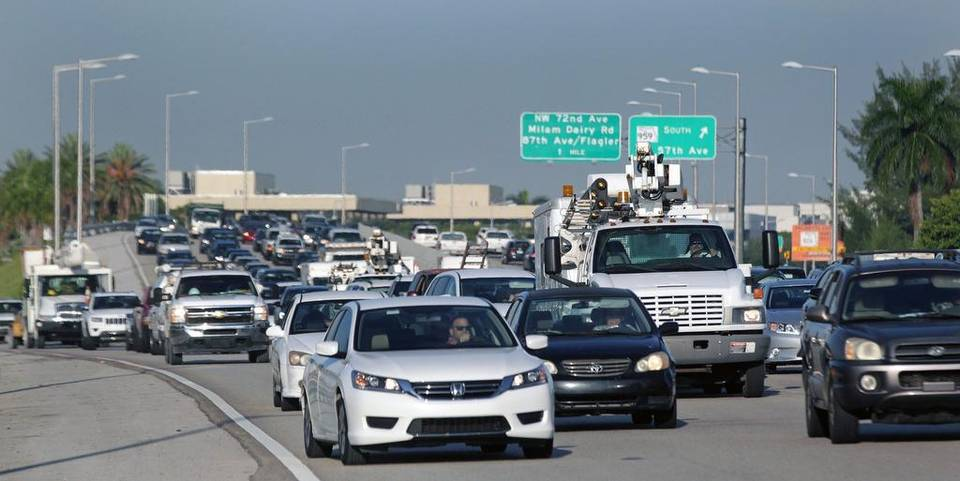
\includegraphics[height=.12\linewidth]{gfx/florida_no_front_number_plates}} \quad
        \subfloat[Alfa Romeo 159 with number plate mounted at the side (reprinted from \footnote{\url{http://www.seriouswheels.com/2008/a/2008-Autodelta-Alfa-Romeo-159-J4-2-2-C-Front-1280x960.htm}})]
        {\label{fig:numberPlateSide}%
         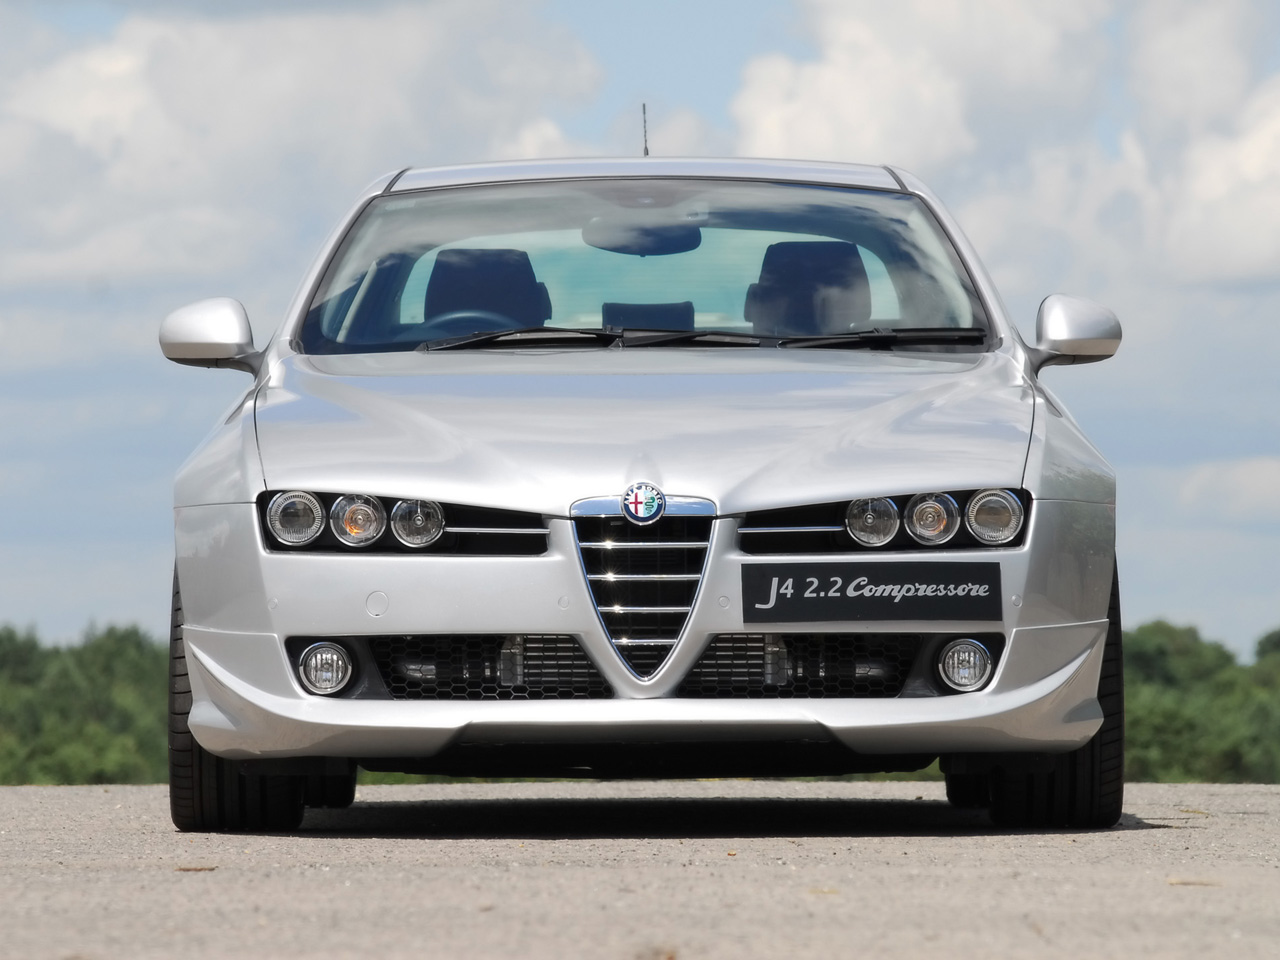
\includegraphics[height=.12\linewidth]{gfx/number_plate_front_side}} \quad
        \subfloat[RoIs of a Porsche 911 (left) and a Volkswagen T6 (right)]
        {\label{fig:roiMaskPorscheT6}%
         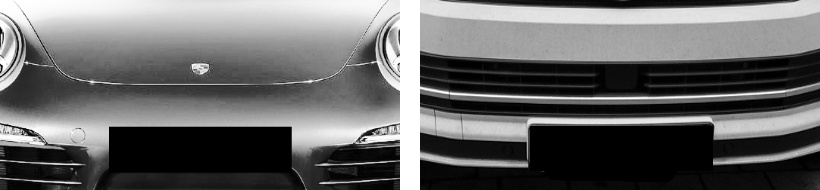
\includegraphics[height=.12\linewidth]{gfx/roi_mask_porsche_t6}}
        \caption[Problems when choosing the front number plate as center of the RoI]{Problems when choosing the front number plate as center of the RoI}
\end{figure}
Using the hood boundary to deduce the RoI's properties would fix the last mentioned problem, because the size of the hood boundary depends on the size of the car. Since the detection of the hood boundary is failure prone and since classifiers trained with RoIs including the hood region performed inferior to those trained without the hood region \citep{hsieh2014symmetrical}, the number plate-approach is chosen for this thesis.

Starting from the front number plate, a RoI can be defined around it that automatically contains descriptive vehicle information. An example for this is illustrated in figure \ref{fig:roiDimensions}.

\begin{figure}[btph]
  \centering
        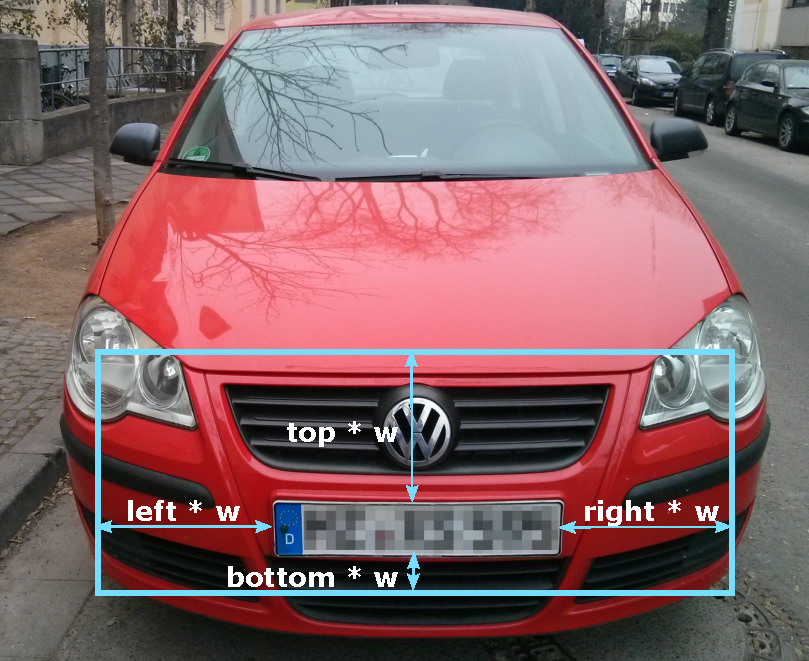
\includegraphics[width=.35\linewidth]{gfx/roi_dimensions}
        \caption{Definition of the RoI extent depending on the width $w$ of the number plate. Concrete values for $left$, $right$, $top$ and $bottom$ have been evaluated in table \ref{table:tunedParameters}}
        \label{fig:roiDimensions}
\end{figure}

\subsubsection{Variations}
There are different possibilities to define the RoI around a number plate, depending on the choice of the values $left$, $right$, $top$ and $bottom$ denoted in figure \ref{fig:roiDimensions}.

\begin{itemize}
  \item Including or not-including the hood region: As shown by \citep{hsieh2014symmetrical}, RoIs including the hood region perform inferior. This might be due to little discriminative information in there. Additionally, the hood might reflect its environment, which puts \emph{negative} information in the resulting descriptor.
  \item Considering only the left (or right) half of the vehicle's front: In general, vehicles are symmetrical. Knowing one half, the other half can be estimated. For a global descriptor built up by concatenating the RoI's pixels, this might help to reduce training and classification time, because the descriptor's length would halve itself without losing information (only losing redundant mirrored half). Since the approach used in this thesis is based on a bag-of-words model, the length of the global descriptor does not depend on the size of the RoI but on the size of the dictionary. Halving the RoI would in contrast to that reduce the ability of the system to cope with partial occlusions (see \emph{VR1}) \citep{siddiqui2015robust}. If the selected half is occluded, there is no chance to recognize the vehicle anyway.
\end{itemize}
\citeauthor{petrovic2004analysis} \citep{petrovic2004analysis} shrinked the RoI in horizontal direction to compensate that the vehicle's structure is a little more redundant in that direction. This also only makes sense if the global descriptor's size depends on the size of the RoI, which is not the case in this thesis' approach.

To sum up, the RoI should exclude the hood region while including all of the informative parts over all makes and models. In addition to that, the full and unshrinked width of the RoI should be used. For concrete values and tests see table \ref{table:tunedParameters}.

\subsection{Local Feature Extraction}\label{sec:localFeatureExtractionConcept}
The next step in the workflow is to extract local features. The local features will be extracted from the preprocessed RoI, which is the output of the previous step.

A local feature is a point in the RoI, that is significant, like a corner. Such features are located via a feature detector (see figure \ref{fig:localFeaturesExample}). After a feature has been detected, it will be encoded by a feature descriptor. A feature descriptor embeds the feature into its surrounding context. As the name says, the feature descriptor's purpose is to describe the found feature such that the same feature can be recovered in another image (see figure \ref{fig:localFeaturesMatchingExample}).

There are many different feature detectors and feature descriptors with different purposes and properties. It turned out that SIFT (Scale Invariant Feature Transform) \citep{lowe1999object} and SURF (Speeded Up Robust Features) \citep{bay2008speeded} are very suitable to describe vehicle features. SIFT and SURF are in some extent invariant to scaling (of course, as the name says) and to rotation, which was requested by \emph{VR2} above. They are also partially invariant to illumination changes and robust to local geometric distortion, which satisfies \emph{VR3} to work under various lighting conditions. But there is one big problem with these feature transformations: They are both patented
%(TODO: only show patent nr. BibTeX has an extra tag for patents)
(\footnote{SIFT patent: \url{https://www.google.com/patents/US6711293}}, \footnote{SURF patent: \url{https://worldwide.espacenet.com/publicationDetails/biblio?CC=US&NR=2009238460&KC=&FT=E&locale=en_EP}}). An alternative for this is proposed with ORB. ORB is said to be rotation invariant and resistant to noise. Furthermore, it's said to be faster than SIFT and in many situations performing equally well \citep{rublee2011orb}. And best of all, it's not patented. So the implementation is based on ORB-features.

The output of this step is a set of local descriptors per RoI. In the figure, each set is represented as a cloud with blue dots, which represent the local descriptors in local-descriptor-space.

\begin{figure}[btph]
  \centering
        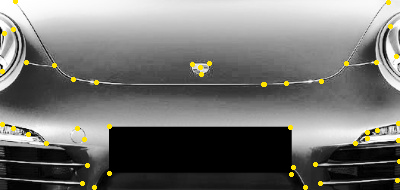
\includegraphics[width=.35\linewidth]{gfx/local_features_porsche}
        \caption{RoI with found local features marked as yellow points}
        \label{fig:localFeaturesExample}
\end{figure}
\begin{figure}[btph]
  \centering
        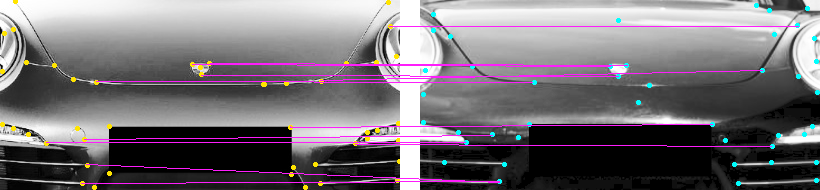
\includegraphics[width=.65\linewidth]{gfx/local_features_porsche_matching}
        \caption{Two RoIs showing different instances of the same car (Porsche 911) with found local feature matches shown as purple lines (also including false matches)}
        \label{fig:localFeaturesMatchingExample}
\end{figure}

\subsection{Dictionary}\label{sec:dictionaryConcept}
Having a collection of local features per RoI, they must be transferred into a global representation in some way. This is where the dictionary comes in.

As said above, this VMMR approach is based on a bag-of-words model, where the dictionary is the \emph{bag} containing the (code-)\emph{words}. Similar local descriptors will be represented by one single codeword, which is then again a local descriptor. Each codeword will then be referred to by the global representation, which provides one histogram bin for each codeword (see \ref{sec:globalRepresentationConcept}). For the global representation to be expressive, each codeword has to be expressive, too. To retrieve codewords, the inputted local descriptors are clustered, whereas each cluster is turned into a codeword.

\citeauthor{siddiqui2015robust} \citep{siddiqui2015robust} investigated in two different schemes of building a dictionary from various vehicle classes' local descriptors (see page \pageref{par:dictionaryGenerationStateOfTheArt}). One scheme was to build a dictionary out of the local descriptors of all vehicle classes, called the \emph{Single Dictionary}. The other scheme was to build one dictionary for each vehicle class and then pooling all the codewords. The latter is called the \emph{Modular Dictionary}. Although the SD has the disadvantage of clustering similar local descriptors but from different vehicle classes into one single codeword (which will cause inter-class ambiguity issues), it performed superior to the MD (according to tests made by \citeauthor{siddiqui2015robust}). As an example, referring to picture \ref{fig:ambiguityPorsche}, descriptors of the round headlights of both, the Mini and the Porsche, could be clustered into the same codeword because of their similarity.

A problem of the Modular Dictionary is its size (see page \pageref{par:dictionaryGenerationStateOfTheArt}). A too large dictionary leads to large global representations. A result of this would be a classifier that misses generalizability and tends to be overfitted\footnote{The classifier would perform well for the images in the training set but would perform worse for unknown images}. Drastically reducing the number of per-class-clusters of the per-class-dictionaries (as \citeauthor{siddiqui2015robust} did) will fix this problem, but will also lose descriptivity of the per-class codewords. This is for one thing, because different features that should also be handled different, are clustered into the same cluster. For another thing, the ratio of useless clusters to informative clusters increases for a low number of clusters (see figure \ref{fig:modularDictionaryClusters}). Useless clusters either contain outlier features (e. g. because of noise) or features that only occur in a small fraction of training images of a specific class. Since clusters are used to create dictionary codewords, which are used to create descriptive global representations of classes, useless clusters are counterproductive.

This thesis introduces a new dictionary scheme as a solution to these problems.

\begin{figure}[btph]
  \centering
        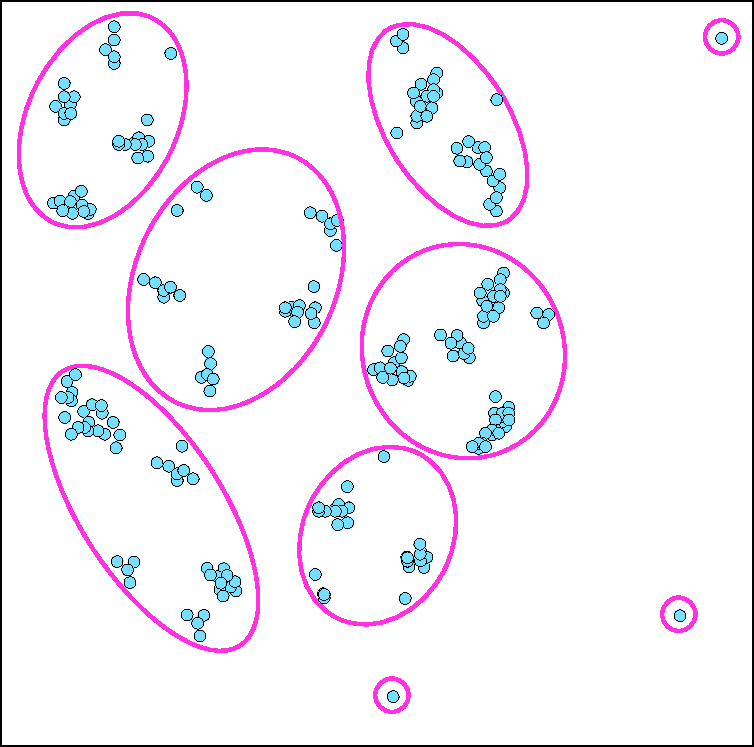
\includegraphics[width=.45\linewidth]{gfx/modular_dict_clusters}
        \caption{Problem with too little per-class-clusters for the MD (showing cluster space for one class): Blue dots represent local descriptors of instances of the class. Purple ellipsoids mark the clusters. Reducing the number of clusters too much raises the importance of clusters that only include few outlier-descriptors.}
        \label{fig:modularDictionaryClusters}
\end{figure}

\subsubsection{Advanced Modular Dictionary}
The Advanced Modular Dictionary (AMD) scheme extends the Modular Dictionary scheme. To solve the problem of too poor per-class-clusters, the per-class-clustering will be performed with a reasonable high number of clusters, whereas after the clustering, only the \emph{good} clusters are kept. To cope with a too large codeword pool inside the Modular Dictionary, the codewords of the per-class-dictionaries are clustered once more.

\begin{figure}[btph]
  \centering
        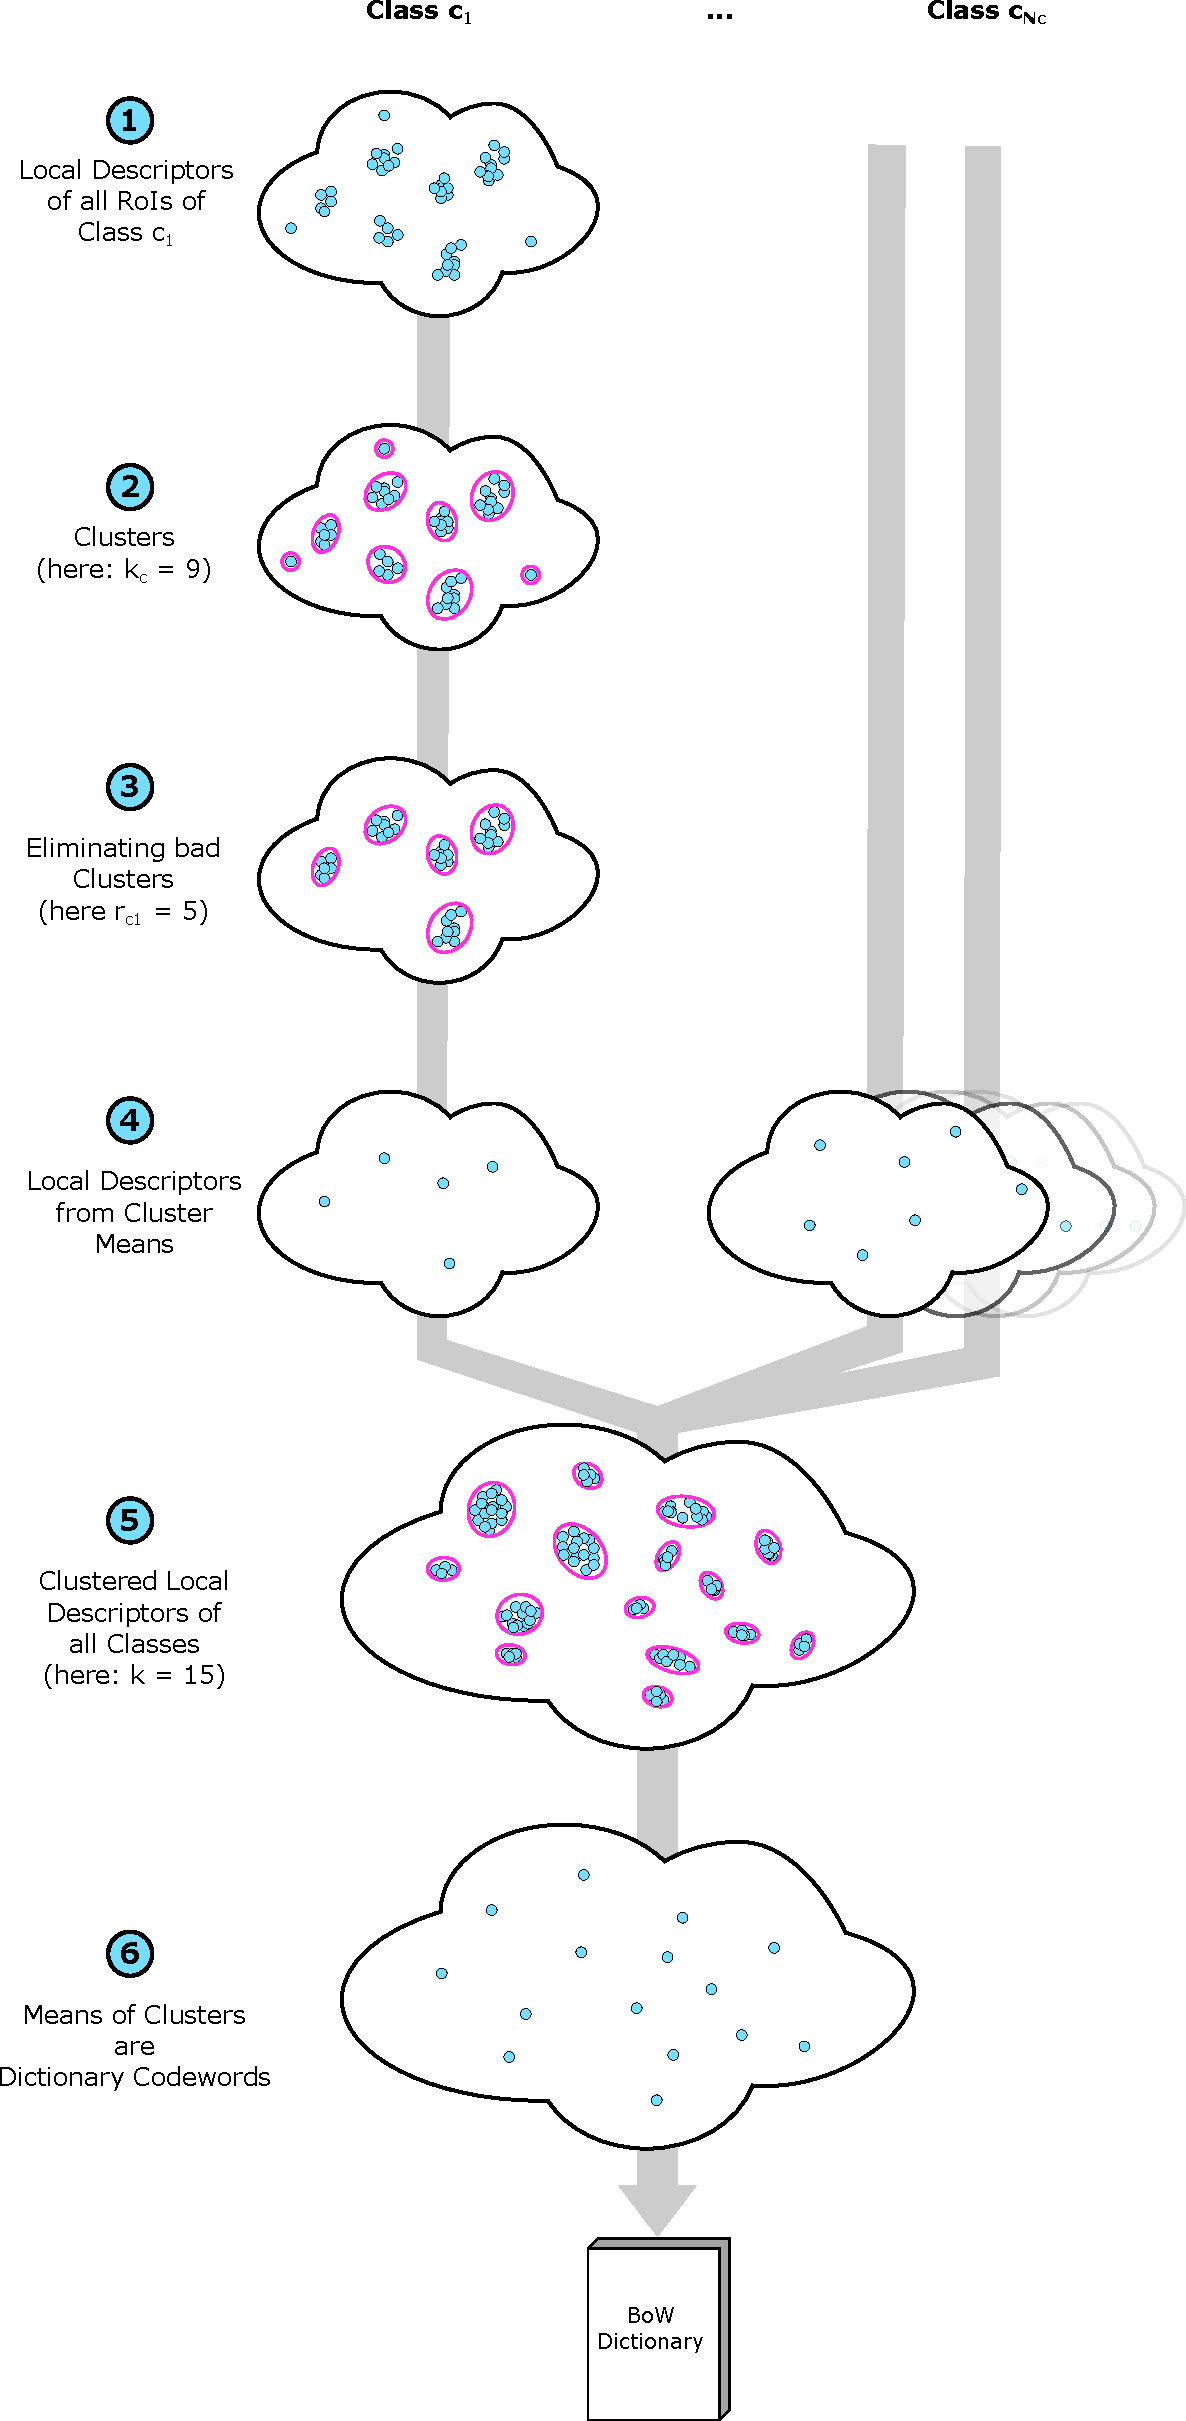
\includegraphics[width=.65\linewidth]{gfx/amd_process}
        \caption{Generation process of the Advanced Modular Dictionary. See text for a detailed description.}
        \label{fig:amdProcess}
\end{figure}

In the VMMR workflow from figure \ref{fig:vmmrWorkflow}, the dictionary generation is described as a process, that gets the local descriptors of all RoIs as input and produces a ready-to-use dictionary as output. In the following, the intermediate steps are explained. Each numbered section refers to the numbered steps from figure \ref{fig:amdProcess}.
\begin{enumerate}
	\item The generation process starts the same way, the Modular Dictionary does: The local descriptors of all instances are gathered class-wise. In the figure, this step is shown exemplarily for class $c_1$. The cloud represents the local-descriptor-space while the blue dots mark the single local descriptors
	\begin{equation}\label{eq:descriptorsRoI}
	f_1^{c_i},\dots,f_{Nf_{c_i}}^{c_i}
	\end{equation}
where $f_j^{c_i}$ represents the $j-th$ local descriptor for the class $c_i$ and $Nf_{c_i}$ is the number of local descriptors of the class $c_i$.
	\item In this step, the local descriptors get clustered class-wise. There is also no difference to the proposed Modular Dictionary creation process up to now, except for the requested number of clusters $k_c$. In contrast to the number evaluated best by \citeauthor{siddiqui2015robust}, which was $29$, the number $k_c$ evaluated best for the AMD is about ten times as large (see table \ref{table:tunedParameters} for evaluation details). For each class $c_i$, this step produces $k_c$ clusters
	\begin{equation}\label{eq:clustersRoI}
	\Omega_1^{c_i},\dots,\Omega_{k_c}^{c_i}
	\end{equation}
where $\Omega_j^{c_i}$ represents the $j-th$ cluster for the class $c_i$. The clusters are represented as purple ellipsoids in the figure.
	\item This step is about separating the \emph{good} clusters from the \emph{bad} ones, as said above, whereas the bad ones will be filtered out. The purpose is to end up with just a few clusters, much less than $k_c$, to prevent the final dictionary from blowing up with codewords. Bad or useless clusters, as said above, are clusters that only contain few descriptors, whereas good clusters contain many descriptors of the same kind. That said, a good cluster represents a feature of the class, that occurs in many training images and hence is expressive for that class. To define a good cluster, the parameter $r_{c_i}$ is introduced, which expresses the number of members, a cluster must have to be regarded as a \emph{good} cluster. $r_{c_i}$ is not the same for each class $c_i$ but depends on the number of training images $N_{c_i}$ of class $c_i$. The parameter $t$ controls the ratio, in how many of the $N_{c_i}$ training images a clustered descriptor has to occur, to be regarded as to describe an expressive feature (resulting into an expressive cluster). So the final expression to reduce the number of per-class-clusters is
	\begin{equation}\label{eq:clustersReduction}
	\Omega_1^{c_i},\dots,\Omega_{l_{c_i}}^{c_i} = \{\,\Omega_j^{c_i} \,\mid\,\, |\Omega_j^{c_i}| \ge r_{c_i},\quad j = 1\dots{k_c} \,\}
	\end{equation}
where $l_{c_i} << k_c$ is the remaining number of good clusters and $r_{c_i} = N_{c_i} * t$.
	\item After having reduced the number of clusters, each cluster of local descriptors is turned into one single local descriptor, defined as the mean of this cluster. So each class is represented by a set of local descriptors, which are the codewords of the per-class dictionaries
	\begin{equation}\label{eq:perClassCodewords}
	{f'}_1^{c_i},\dots,{f'}_{l_{c_i}}^{c_i} = mean(\Omega_1^{c_i}),\dots,mean(\Omega_{l_{c_i}}^{c_i})
	\end{equation}
	\item Here, the results of the processes for the other classes are taken into account. For each class, there is a set of codewords $f'_{c_i}$ now, which have been filtered to be expressive for their class. Analogously to step 1, which gathers the local descriptors $f$ of all RoIs class-wise, the codewords $f'$ are gathered over all classes, resulting into a set
	\begin{equation}\label{eq:allDescriptors}
	{f'}_1^{c_1},\dots,{f'}_{l_{c_1}}^{c_1},\quad\dots,\quad{f'}_1^{c_{N_c}},\dots,{f'}_{l_{c_{N_c}}}^{c_{N_c}}
	\end{equation}
where $N_c$ is the number of classes. This equation is similar to the set from equation \ref{eq:descriptorsRoI}, but expresses the whole training set instead of just one single class.

For the MD scheme, the set from equation \ref{eq:allDescriptors} already forms the codewords of the final dictionary. But to cope with the large amount of resulting per-class descriptors $f'$, a further clustering process is deployed. In contrast to the reduction process from equation \ref{eq:clustersReduction}, for this clustering it's good, if a cluster contains a few local descriptors. Because this means, that the resulting codeword only occurs in a few classes. So an amplitude for such a codeword in a global representation histogram gives a useful clue to the classes, the instance could correspond to. A cluster containing a local descriptor of each class is useless, because the resulting codeword would encode each class likewise. So an amplitude to that codeword by a global representation does not tell anything about the class-belonging.

To control the clustering process, a further degree of freedom (the desired number $k$ of resulting clusters) is introduced. With a small value for $k$, it's possible to shrink the number of codewords drastically while losing a lot of per-class information. A large value for $k$ will leave many descriptors untouched by creating one-member-clusters. A special case is, if the value for $k$ equals the number of inputted descriptors, which has the same behavior as the Modular Dictionary scheme. The evaluation of the best value for $k$ will be discussed in the implementation chapter \ref{sec:parameterTuning}.
	\item Finally, the means of the resulting $k$ clusters are turned into local descriptors, as it is done in equation \ref{eq:perClassCodewords}. Each resulting local descriptor represents one of the $k$ codewords $cw$ of the Advanced Modular Dictionary:
	\begin{equation}\label{eq:finalCodewords}
	{cw}_1,\dots,{cw}_k = mean({\Omega'}_1),\dots,mean({\Omega'}_k)
	\end{equation}
where ${\Omega'}_j$ represents the $j-th$ cluster from step 5.
\end{enumerate}

\subsection{Global Representation}\label{sec:globalRepresentationConcept}
The purpose of the global representation is to describe the vehicle instance with all its specific properties, such that a classifier can understand it. A classifier can handle data instances that consist of a set of attributes. Each attribute is of a specific data type, either \emph{nominal} (which has no order, like \emph{color}), \emph{ordinal} (which can be ordered, like \emph{size} with values \emph{small}, \emph{medium} and \emph{big}), or \emph{numeric} (which can be measured, like \emph{number of seats}). A global representation must be expressible via such an instance.

Because of the above mentioned downsides, a simple transformation of the image's pixels into the global representation (the instance would have one numeric pixel value for each attribute) will not be used here. A bag-of-words-based representation can better handle partial occlusions and changes of the camera angle. For this reason, a dictionary was built to project the local descriptors, extracted from the vehicle image, onto dictionary (code-)\emph{words}. This is usually done by storing the word-frequencies in a histogram.

Generating the dictionary and training the classifier don't run in parallel, which could be misinterpreted by the illustration of the training-workflow in figure \ref{fig:vmmrWorkflow}. Since the (complete) dictionary is needed to encode the global representations, the training-workflow firstly generates the dictionary from the local descriptors of all RoIs. After that, the training-workflow runs again by using the existing dictionary to train the classifier.

For a given RoI $r$ and its set of local descriptors $F^r$, the corresponding global representation $H$, the histogram, is a vector that has an entry for each dictionary codeword $cw$. Each entry $H_i^r,\,i = 1..k$ represents the number of local descriptors $f \in F^r$, that are closest to the respective dictionary codeword $cw_i$:
\begin{equation}
H_i^r = |\{\, f \in F^r \,\mid\, dist(f, cw_i) < dist(f, cw_j) \quad \forall i, j: 1 \le i, j \le k,\, i \ne j \,\}|
\end{equation}
As distance measure $dist$, this thesis uses the Hamming distance. Figure \ref{fig:histogram} illustrates the generation of a histogram exemplarily.

\begin{figure}[btph]
  \centering
        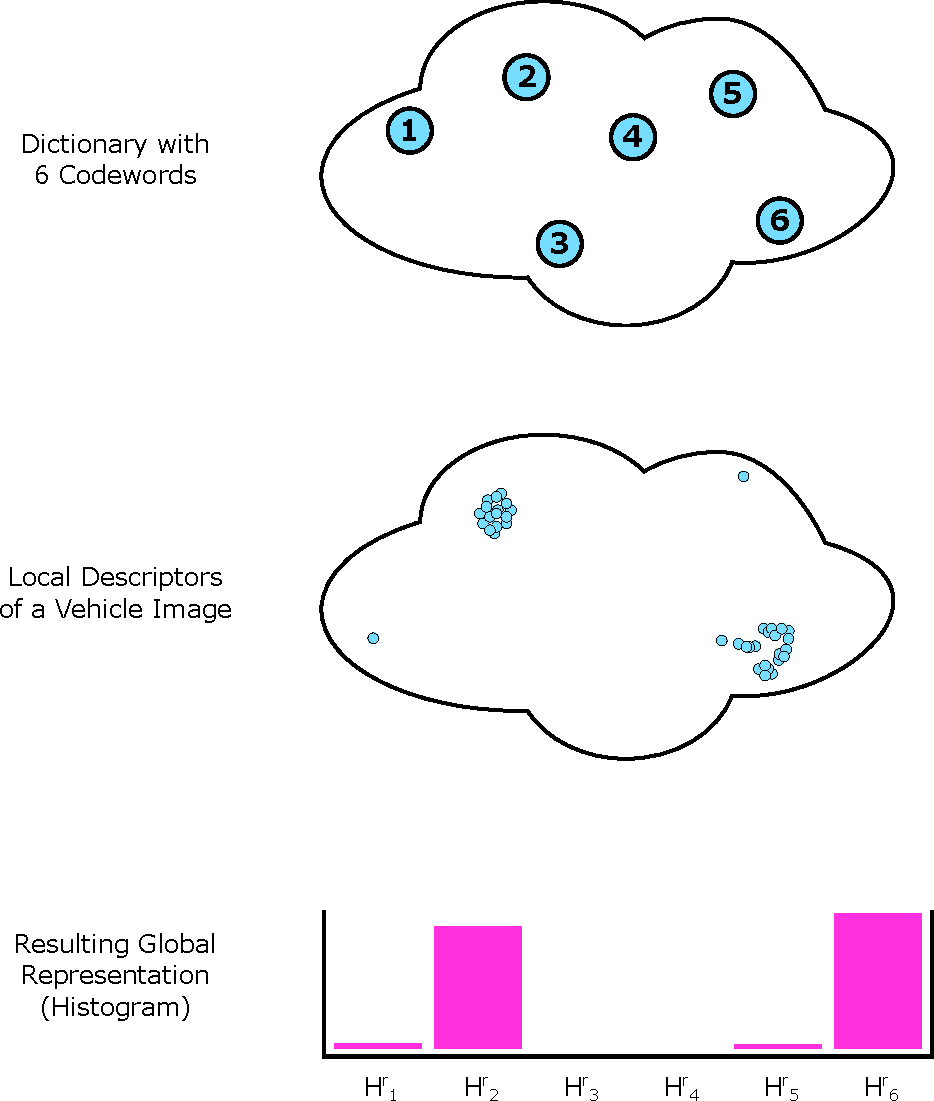
\includegraphics[width=.45\linewidth]{gfx/histogram}
        \caption{Generation of a global representation Histogram: The upper cloud represents the dictionary space with six codewords. The cloud below contains the local descriptors found in a vehicle image. The bottommost figure shows how a histogram for this image would look like.}
        \label{fig:histogram}
\end{figure}

\subsection{Classification}\label{sec:classificationConcept}
The job of a classifier is to assign a class to an unknown instance. To be able to do this, the classifier is trained beforehand with instances and corresponding classes. The instances, the classifier is trained with, are the resulting global representations of the training workflow. With these, the classifier learns how to differ the classes based on the instances' attributes.

There are many different kinds of classifiers, like tree- or rule-based ones, neural networks or SVMs. A description of the various classifiers and their inner processes is not part of this thesis. It has just to be said, however, that different classifiers have their pros and cons, including the training or classification speed, the amount of storage needed, the adaptability for new training data a. s. o.

Concerning the adaptability for new training data: For RacecAR GO, the classifier should be ready to be trained online, i. e. training the classifier is a never-ending process. The classifier is constantly fed with new training data and improves its performance. Since there arrives a new vehicle image with every captured vehicle during play, retrieving new training instances is easy. To get the class label for the new training instance, the classified label could be used, as long as the classification is certain enough. If not, the player could be asked if the classification was correct. If not, the instance could be stored apart to be classified manually by the designer.

For time reasons during the implementation, the classifier of the prototype is trained solely offline, i. e. during the implementation phase of the game. So the classification performance will not change during play. This has the advantage of a reliable and known recognition performance. The disadvantage is, that the classifier cannot improve its performance by adopting new training data.

For the actual decision of the classifier, see chapter \ref{sec:classificationImpl}.

\subsection{Choice of Vehicle Classes}\label{sec:choiceOfVehicleClasses}
As mentioned in the concept for RacecAR GO, the prototypical version of the game that is implemented within this thesis' scope will only cover a subset of all the world's makes and models, i. e. 10 different make-model-classes. The choice of the actual classes plays a role because of the following reasons:
\begin{itemize}
  \item Control of multiplicity and ambiguity issues: As defined in \emph{VR4}, the VMMR has to be able \emph{"to cope with ambiguity and multiplicity issues"}. The choice of vehicle classes affects the discriminability of the different makes and models. Choosing 10 vehicle classes with high inter-class differences will increase the discrimination power of the VMMR. This is of no relevance with regard to a final version of the game, where all the world's makes and models shall be covered. But as long as this isn't the case, the covered vehicles have to be recognized as well as possible. As an example, choosing both, a Porsche and a Mini to be recognized by the VMMR system is a bad choice due to high inter-class ambiguity issues between these classes (see picture \ref{fig:ambiguityPorsche}). Thus the target is to achieve a distribution of dictionary codewords, where each codeword encodes as few classes as possible while the pairwise distance among the codewords is as large as possible.
  
  For local descriptors $f^{c_i}$ and $\hat f^{c_i}$ of class $c_i$, let
  \begin{equation}
  E^{c_i} = \sum_{f^{c_i}, \hat f^{c_i}} dist(f^{c_i},\hat f^{c_i})^2 \quad \forall f^{c_i}, \hat f^{c_i}
  \end{equation}
  be the intra-class error of class $c_i$ and
  \begin{equation}
  E = \sum_{i, j = 1}^{\hat N_c} dist(mean(c_i), mean(c_j))^2
  \end{equation}
  be the inter-class error, where $\hat N_c > N_c$ is the number of classes with available training data and $mean(c)$ is the mean of all local descriptors of class $c$. Then the task is to maximize $E$ while minimizing $E^{c_i} \, \forall i = 1,\dots,N_c$ for all possible combinations of $N_c$ different classes:
  \begin{equation}\label{eq:optClasses}
  K_{opt}^{N_c} = \argmin_{\{c_1,\dots,c_{N_c}\} \,\in\, perm_{N_c} \, K} \frac{\sum_{i = 1}^{N_c}E^{c_i}}{E}
  \end{equation}
  where
  
  \begin{tabular}{ll}
  $K$                     & set with all classes with available training data, $|K| = \hat N_c$ \\
  $K_{opt}^{N_c}$         & subset of $K$ with $N_c$ classes with optimal distribution \\
  $perm_{N_c}$            & function that generates all possible permutations of size $N_c$ \\
  \end{tabular}
  \item Availability of chosen classes in the player's surroundings: To keep the fun of play, the game must recognize vehicles, that frequently occur in those areas, the game will be played in. Additionally, the game should represent some seldom cars to challenge the players to be on the prowl for them. If the game supports too many frequent cars, the player could lose fun because of the missing challenge. If there are too little, the player could be too challenged. So to hold the player in flow, the set of represented classes should thus consist of a reasonable ratio of frequent and seldom vehicle classes. For this reason, the training data solely consists of vehicles occurring in Germany (where the prototype will be tested), some of them are frequent (like a VW Golf IV), others are rare (like a Porsche 911).
  \item Last but not least, photos of these vehicles must exist to train the VMM recognizer. The problem with seldom cars is that one rarely sees them on the street or at public car parks. In contrast to that, there's no problem to find vehicles of frequent classes.
\end{itemize}







%*****************************************************************************
%*****************************************************************************
\chapter{Implementation}\label{ch:implementation}
%*****************************************************************************
%*****************************************************************************
\section{Overview}
This chapter is about implementations of some of the components and algorithms, described in the Concept chapter. It's subdivided into one part for the server implementation, one for the network interface and one for the client implementation. The server chapter also includes an evaluation of the VMMR machine at the end.

The source code can be found at following locations:
\begin{itemize}
  \item Server component, including the implementation of the VMMR: \url{https://github.com/johannesheucher/VehicleFeatureExtractor}
  \item iOS app: \url{https://github.com/johannesheucher/RacecAR_GO_Client}
  \item Dataset, created along with this thesis: \url{https://github.com/johannesheucher/VehicleData}
  \item Vehicle collector app to fill the dataset: \url{https://github.com/johannesheucher/VehicleCollector}
\end{itemize}


\section{Server}
Figure \ref{fig:platform} says, that the server takes care for tasks like VMMR, the user management and the game state. Since the prototype is mainly limited to the capturing of vehicles, the only part left for the server is the VMMR.

The recognition is realized as a machine learning system, that trains a classifier based on labeled training images. In this chapter, the several components along with implementation details will be described. The order of described components equals the order denoted in the VMMR workflow in figure \ref{fig:vmmrWorkflow}.

The Server is realized as a Java application. For image processing, OpenCV 3\footnote{\url{http://opencv.org/}} is used. OpenCV is a commonly used library for computer vision purposes. It is implemented in C, but it was ported to be used with Java or Objective-C on many platforms. For training the final classifier, Weka 3.8\footnote{\url{http://www.cs.waikato.ac.nz/ml/weka/}} is used. Weka provides a set of classifiers of different kind and useful functions to train them.

The performance of the VMMR strongly depends on the choice of parameters. There are many configurations to make, from the size of the RoI through the size of the dictionary to parameters of the final classifier. To find suitable parameters for a good performance, an automatic parameter tuning is used, which is presented in chapter \ref{sec:parameterTuning}.

\subsection{Dataset}\label{sec:dataset}
The VMMR workflow starts with a set of training images, the dataset. In this case, the training images are pictures of cars with make-model labels assigned. As described in chapter \ref{sec:vmmrConcept}, there are different criteria, the training images have to fulfill:
\begin{itemize}
  \item The decision was made to recognize a car only by its front. So the training images need to depict the front of a vehicle. Retrospectively, it would have been better to choose the vehicle's backside. This would at least have simplified the collecting of training data, because most people pull into a parking space.
  \item Since the main application area is Germany (at least for the initial launch of the app), pictures of vehicles occurring in Germany should be included. It should be a reasonable mix of frequent and rare make-models.
  \item For the prototype, the limitation has been made to solely recognize cars and no trucks, buses, motorbikes, etc. So the training set should be specialized to cars.
  \item The per-class images should vary lightning- and weather-conditions. As requested by \emph{VR3}, the recognizer shall be independent from lighting to prevent making the same mistake as the recognizer of tanks, that recognizes cloudy and sunny instead. To fulfill this request, the recognizer has to learn a large variance of lighting conditions for each vehicle class.
  \item The cars on the per-class images should be as diverse as possible to cover all variants of that specific vehicle class. E. g. a VW Golf VII is available as standard Golf, as GTI, GTD, GTE, e-Golf or Golf R, all slightly differing in the front.
  \item The perspective of the picture, though frontal, should also vary to be prepared to cope with different view angles and player sizes during the capturing process.
  \item The pictures must be occlusion-free.
\end{itemize}
It is also possible to use the same real vehicle multiple times inside the training data, as long as it has been photographed under different lighting conditions or view perspectives.

Since I'm not the first one to train a VMMR, there already exist datasets for this purpose. For example, there's the NTOU-MMR dataset \citep{ntoummrDataset} that is used by \citep{siddiqui2016real} or another dataset used in the work \citep{krause20133d}. Unfortunately, both datasets mostly consist of pictures of vehicles made in the USA. Though there are vehicles that are also available in Germany (like the Toyota Yaris), most of them aren't. Additionally, the latter dataset's pictures don't show purely frontal views of vehicles but also pictures from the side or the front-side. As a result, there wasn't any dataset available that fitted the needs denoted above. So an own dataset was created along with this thesis.

\subsubsection{Dataset Creation}\label{sec:datasetCreation}
To save time and improve the diversity of available vehicle classes, an extra app has been created to take photos of vehicles along with the corresponding make and model. The app has been spread among some of my friends with the request to take as many pictures as possible while regarding the above-mentioned criteria. An advantage is, that these pictures are taken with ordinary smartphone cameras, so the quality of the images equals that one of those pictures, taken by the RacecAR GO app during the capturing process. Such a collector app has the further advantage that it reminds the training data collectors to collect training data, because they always see the app when looking on their smartphone. The app stores these pictures locally with the make, model and a time stamp as file name, so that the collectors only had to push the collected images onto a web storage regularly.

As a result, the final dataset consists of 313 vehicle pictures, 11 different makes and $\hat{N_c} = 24$ different make-model classes. Their original sizes vary from 5312 x 2988 to 554 x 444 pixels. Actually, many more make-models have been photographed, but only those classes with a reasonable amount of images per class (at least six) made their way into the dataset. Make-models of the dataset are: Citro\"en C4 Cactus, Ford Fiesta, Ford Fiesta (FL), Mazda MX-5 ND, Mercedes A, Mini One R55, Opel Adam, Opel Astra H, Opel Astra H (FL), Opel Corsa D, Opel Corsa D (FL), Opel Mokka, Porsche 991, Skoda Fabia II, Skoda Octavia, Suzuki Swift MZ, Tesla Model S, VW Golf IV, VW Golf, VI, VW Golf VII, VW K\"afer, VW Polo 6R, VW Polo 9N3, VW UP.

Unlike \citep{siddiqui2015robust} who trained the classifier to learn similarities among facelifts of the same make-model class, this approach splits each facelift of a make-model into a different class (e. g. there's the \emph{Opel Corsa D} and the \emph{Open Corsa D (FL)}). Building a classifier that regards facelifts inside one make-model generation as one single class turned out to decrease the classification accuracy due to multiplicity issues.

\subsubsection{Supported Vehicle Classes}\label{sec:supportedVehicleClassesImpl}
In Chapter \ref{sec:choiceOfVehicleClasses}, an approach has been presented to retrieve a set of those classes that cope best with ambiguity and multiplicity issues. Instead of using all $\hat{N_c} = 24$ classes, the training set contains pictures for, only $N_c = 10$ of them with best discriminability are chosen to be covered by the prototype. As described in equation \ref{eq:optClasses}, calculating the errors and building the $argmin$ over all possible subsets with size $N_c$ yields the desired ten vehicle classes that will be used to train the VMMR with.

The ten classes, evaluated by the proposed approach, are: Citro\"en C4 Cactus, Ford Fiesta, Mazda MX-5 ND, Opel Corsa D (FL), Opel Mokka, Porsche 991, Tesla Model S, VW Golf IV, VW K\"afer, VW Polo 9N3. The features $f^{c_i}$ to calculate the per-class errors $E^{c_i}$ and the class means were taken from the normalized RoIs. The total number of training instances for these classes is 189.

\subsection{Region of Interest}
To extract the RoIs of the training images, each number plate has been marked manually. The position and size of each image's number plate is stored in a separate file, coming along with the dataset. When loading the dataset, the data structure for each image retrieves this data, such that it can export the RoI.

The RoI is defined by two properties, the content extent $RoI_E = (top, bottom, left, right)$ and the size in pixels, whereas for the size only the width $w_{RoI}$ is important. The height is deduced from $w_{RoI}$ and the aspect ratio of the extent. This means, that the RoIs of all the training images have the same size. This is important for comparable image operations like detecting or describing features. The filter kernels used for this have a distinct size and the car in each image should cover a more or less constant percentage of area of the image. The best width has been evaluated to $w_{RoI} = 400$, whereas the extent was evaluated to work best with $top = 0.7, bottom = 0.1, left = 0.6, right = 0.6$. See chapter \ref{sec:parameterTuning} for details to the parameter evaluation process.

%TODO low: Algorithm to find number plate (see doc)

\subsection{Preprocessing}\label{sec:preprocessingImpl}
In \emph{VR3}, the VMMR was requested to be robust to different lighting conditions. To cope with this on the one hand, the training images should cover a large variety of different lighting conditions. On the other hand, the images have to pass a normalization step before entering the training process. To be independent from different vehicle colors, all training images are turned into grayscale images. It also turned out to improve the recognition accuracy, if the contrast is normalized as well by a histogram equalization.
%An illustration of the training data at this point of state is shown in figure TODO Bild zeigen, wie die Trainingsdaten zu diesem Zeitpunkt aussehen (d.h. Bild mit allen RoIs des Trainingsets aus /training2)

\subsection{Local Feature Extraction}\label{sec:localFeatureExtractionImpl}
As described in chapter \ref{sec:localFeatureExtractionConcept}, the common and popular feature detectors and descriptors SIFT and SURF are patented. As a solution, ORB is another feature detector and descriptor, that is faster than SIFT and performs equally well in many situations \citep{rublee2011orb}. Fortunately, ORB is not patented and is included in OpenCV 3.

Unfortunately, both SIFT and SURF are not even included into OpenCV 3, so a comparison among these three regarding VMMR has not been done.

\subsection{Dictionary}\label{sec:dictionaryImpl}
On page \ref{par:dictionaryGenerationStateOfTheArt}, two different schemes of generating the bag-of-words dictionary have been described, the Single Dictionary and the Modular Dictionary. In chapter \ref{sec:dictionaryConcept}, a further scheme, the Advanced Modular Dictionary, was proposed. Within this thesis, both the Single Dictionary and the Advanced Modular Dictionary have been implemented for a comparison.

For both, the Single Dictionary and the Advanced Modular Dictionary, the underlying data structure is an array of (ORB) feature descriptors (the codewords). They only differ in the generation process.

\subsubsection{Implementation of the Advanced Modular Dictionary}
\paragraph{Parameters:}
\begin{itemize}
  \item Number of per-class dictionary codewords $k_c$
  \item Minimum population ratio $t$
  \item Number of final dictionary codewords $k$
\end{itemize}
To cluster the descriptors of the extracted features per class, the clustering algorithm \emph{k-means} is used. OpenCV provides an implementation for this algorithm, called with
\begin{verbatim}
  kmeans(descriptors, k, labels, termCriteria, attempts, flags, vocabulary)
\end{verbatim}
The per-class clusterings are called each with the respective class-descriptors, the number of desired clusters $k_c$, an \texttt{attempts}-value of $1$ and as termination criteria a maximum count of $1000$ algorithm steps. The \texttt{flags}-parameter specifies the kind of initial cluster centers, which has been set to \texttt{KMEANS\_PP\_CENTERS}. The resulting cluster centers are stored in the \texttt{vocabulary}-parameter and represent the per-class dictionary codewords.

After the clustering is done, the minimum population value is calculated for each class with $r_{c_i} = N_{c_i} * t$. The output parameter \texttt{labels} represent a mapping for each descriptor to its containing cluster. They are used to find those clusters (-centers), that have to be eliminated because of a population count $< r_{c_i}$.

For a RoI size of 400 x 190 pixels, there are about 400 features found with the ORB detector. A good value for $k_c$ has been evaluated to $320$ (by the parameter optimizer). For $t$, a value of $0.85$ is optimal, which requires a minimum population of $17$ descriptors for a class with $20$ instances. With these values, between 5\% and 50\% of clusters with too few descriptors have been eliminated for each class.

For the second clustering, that clusters the per-class codewords, k-means is used again. The same parameters as above are used, whereas the value for $k$ was evaluated to $500$ by the parameter optimizer. With a number of $2594$ total codewords from the per-class dictionaries after the elimination process, it turns out that the clustering of codewords belonging to different classes (which was the inter-class ambiguity problem of the SD) seems to be acceptable up to a certain amount.

Especially a configuration of the parameters like ($k_c = 29$, $t = 0$, $k = k_c * N_c = 290$), which represents the standard MD as it has been configured by \citep{siddiqui2015robust}, is inferior to the AMD used with the described parameters.

\subsubsection{Implementation of the Single Dictionary}
\paragraph{Parameters:}
\begin{itemize}
  \item Number of dictionary codewords $k$
\end{itemize}
To cluster the descriptors from all extracted features, k-means is used with the same configuration as described above. The optimum value for $k$ was evaluated to $450$ for the SD.

The built dictionary is finally exported into a file. The server application imports this dictionary to generate the global representations of the queried vehicle instances.

\subsection{Global Representation}\label{sec:globalRepresentationImpl}
The global representation is implemented as an array of doubles, where each entry represents the number of (normalized) matches of found descriptors with the respective dictionary codeword. The OpenCV function
\begin{verbatim}
  DescriptorMatcher.create(DescriptorMatcher.BRUTEFORCE_HAMMINGLUT)
\end{verbatim}
is used for this, using the Hamming distance as distance measure. To train a classifier with the global representations, they have to be converted into a format, the classifier understands. Since this thesis uses Weka for classification purposes, the histograms have to be converted to the ARFF format, which describes a list of instances sharing a set of attributes. The attributes are represented by the dictionary codewords (numeric attributes) plus an additional nominal attribute to hold the make-model class. So each instance is listed inside of the ARFF file as a list of histogram values and the respective make-model class.

\subsection{Paramter Tuning}\label{sec:parameterTuning}
This chapter is about the tuning of the aforementioned VMMR parameters and the selection of the classifier performing with the best accuracy. The tuning is done within an automatic process, which evaluates different values for each parameter to finally retrieve the parameter set with the best performance. The parameters that are tuned are listed in table \ref{table:tunedParameters}. For each parameter, a set of discrete possible values was defined. The tuning process tests all combinations of possible values and yields the best ones. As measure for the best parameter setup, the classification accuracy is used, which is defined as the portion of correctly classified instances (\emph{true positives} and \emph{true negatives}) to the totally classified instances. The accuracy is evaluated via a 5-fold cross validation, i. e. there's no explicit test set.

\subsection{Querying}
For the querying, the server receives a captured vehicle RoI from the client. So the query-process on the server-side begins with the preprocessing of the queried RoI (cf. figure \ref{fig:vmmrWorkflow}). Each client query is processed in a separate thread. As soon as the query workflow has finished and the make-model of the queried instance has been determined, the result gets sent back to the client.

\subsection{Results}\label{sec:results}
In table \ref{table:tunedParameters}, all the parameters that are passed to the tuning process are listed. For each parameter, the possible values, the tuner has to test, are specified as well as the resulting optimum value.
\begin{table}[btph]
    \centering
    \begin{tabular}{ | l | p{4cm} | p{6cm} | l |}
    \hline
    \textbf{Name} & \textbf{Description} & \textbf{Possible Values} & \textbf{Optimum Value} \\ \hline
    $w_{RoI}$    & Width of each RoI in pixels      & {200, 250, 300, 350, 400, 450, 500, 550, 600, 800} & 400 \\ \hline
    $top$      & Top factor for the RoI extent    & {0.6, 0.7, 0.9, 1.4}                               & 0.7 \\ \hline
    $bottom$   & Bottom factor for the RoI extent & {0, 0.1, 0.2}                                      & 0.1 \\ \hline
    $left$     & Left factor for the RoI extent   & {0.6, 0.8, 0.9}                                    & 0.6 \\ \hline
    $right$    & Right factor for the RoI extent  & {0.6, 0.8, 0.9}                                    & 0.6 \\ \hline
    $k$        & Total number of codewords in the dictionary & {250, 290, 350, 400, 450, 500, 550, 600} & 500 \\ \hline
    $k_c$      & Number of codewords in the per-class dictionaries & {29, 80, 150, 200, 270, 300, 320, 350, 400} & 320 \\ \hline
    $t$        & Minimum cluster population ratio for elimination process & {0, 0.3, 0.6, 0.85, 0.95}  & 0.85 \\ \hline
    classifier & Classifier used for VMMR classification & {SVM, Random Forest, Neural Network}        & SVM \\ \hline
    \end{tabular}
    \caption{VMMR parameters for tuning and the evaluated optima (using the AMD)}
    \label{table:tunedParameters}
\end{table}
For the classifiers, there are further sub-parameters, where possible values have been specified for. These sub-parameters and their possible values have been omitted in the table.

The resulting accuracy, using the Advanced Modular Dictionary, is 72.5\% with a precision of 73.1\%. This process has also been done using the Single Dictionary, resulting in an accuracy of 70.4\%, so the SD performs slightly inferior to the AMD. The classification results for the several classes are listed in table \ref{table:classificationResults}.
\begin{table}[btph]
    \centering
    \begin{tabular}{ | l | l | l |}
    \hline
    \textbf{Class} & \textbf{True Positive Rate} & \textbf{False Positive Rate} \\ \hline
    Opel Corsa D (FL)  & 0,800 &  0,011 \\ \hline
    VW K\"afer & 	0,385 &  0,017 \\ \hline
    VW Polo 9N3  & 	0,926 &  0,037 \\ \hline
    Mazda MX-5 ND  & 0,682 &  0,054 \\ \hline
    Opel Mokka & 	1,000 &  0,000 \\ \hline
    Ford Fiesta  & 	0,308 &  0,006 \\ \hline
    Porsche 991  & 	0,533 &  0,017 \\ \hline
    Tesla Model S  & 0,792 &  0,085 \\ \hline
    Citro\"en C4 Cactus & 	0,652 &  0,042 \\ \hline
    VW Golf IV  & 	0,906 &  0,045 \\ \hline
    \end{tabular}
    \caption{Classification results (using the AMD)}
    \label{table:classificationResults}
\end{table}
The training of the classifier with 189 training images took about 7 seconds, while the classification of one instance averagely took 25 milliseconds. This has been evaluated on an Intel(R) Xeon(R) CPU E3-1230 V2 @3.30GHz.

The bad accuracy in comparison to other VMMRs, which usually performed at accuracies better than 90\% \citep{petrovic2004analysis} \citep{siddiqui2015robust}, could be caused by different factors:
\begin{itemize}
  \item The used training set is rather small in comparison to e. g. the NTOU-MMR dataset \citep{ntoummrDataset}, which contains 2846 images for training, and 3793 images for testing for a total number of 29 classes. The VMMR has been tested at different stadiums of the training data and such with different numbers of training images. It turned out, though, that an increasing number of training images also increases the VMMR accuracy.
  \item The quality of the training data could be better. Maybe, the variance between the per-class images is too high. Additionally, there are some vehicles with mirroring effects on their front, which could have brought some noise into the classification space.
  \item Splitting the data explicitly into a training and testing set instead of using cross validation could increase the accuracy. But with such a small dataset, each instance is needed for training, so cross validation was used.
  \item It could also be caused by the usage of ORB detectors and descriptors. According to \citep{rublee2011orb}, ORB performs equal to SIFT in many scenarios. But in contrast to SIFT and SURF, ORB isn't established in the domain of VMMR, yet and no explicit tests have been made to compare ORB with SIFT and SURF on vehicle images.
  \item The clustering with k-means uses generated initial cluster centers. It hasn't been evaluated, if randomly or manually placed centers would improve the result.
\end{itemize}

\subsubsection{Robustness}
It has been said that the VMMR uses a bag-of-words model to be able to recognize vehicles that are partially occluded. The VMMR has also been requested to be independent of different lighting conditions. Tests have proven, that this is actually the case. Figure \ref{fig:tests} illustrates some vehicles in problematic scenarios (occlusions, bad lighting conditions) and their classifications. In most cases, classifications under bad lighting conditions are correct. And if a vehicle is occluded, there are usually enough descriptive features left in the captured photo to find the correct class (in some cases with occlusions of up to 50\% of the vehicle).

\begin{figure}[btph]
        \myfloatalign
        \subfloat[Golf IV]
        {\label{fig:test1}%
         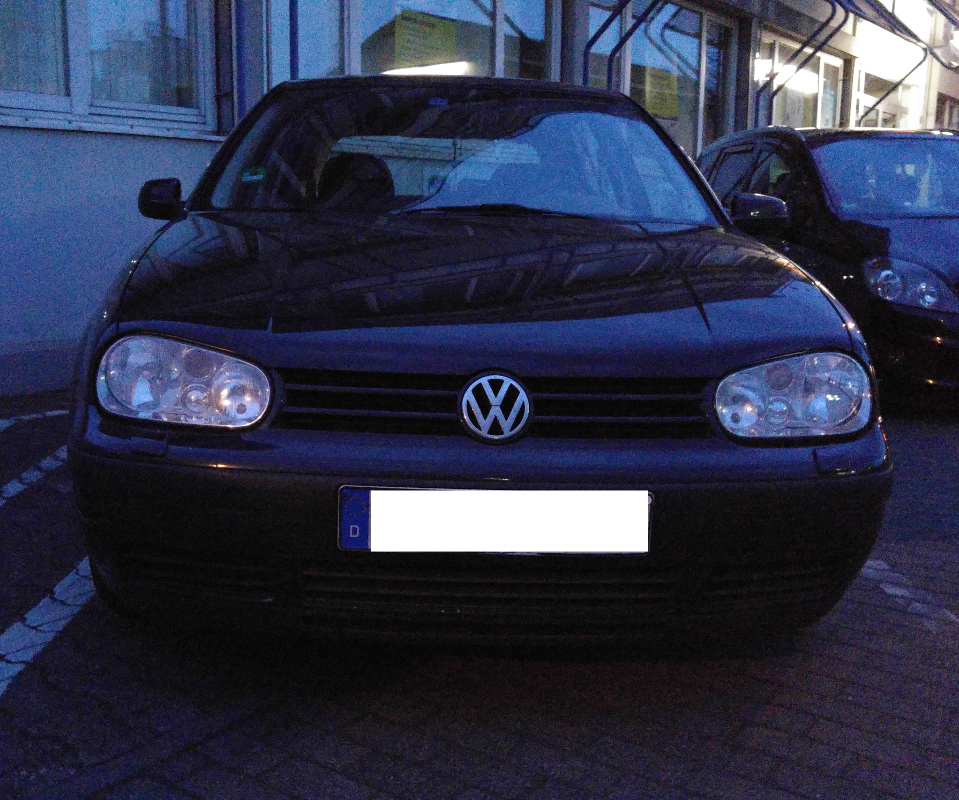
\includegraphics[height=.25\linewidth]{gfx/test1}} \quad
        \subfloat[Citro\"en C4 Cactus]
        {\label{fig:test2}%
         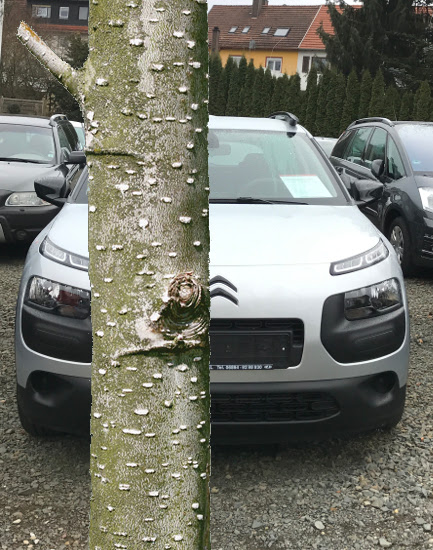
\includegraphics[height=.25\linewidth]{gfx/test2}} \quad
        \subfloat[VW Golf IV]
        {\label{fig:test3}%
         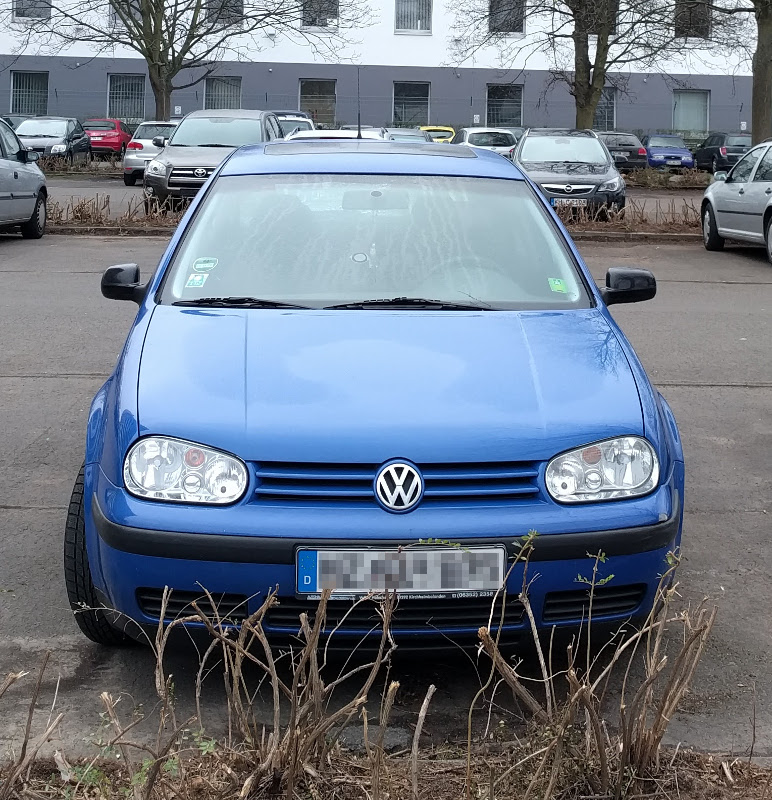
\includegraphics[height=.25\linewidth]{gfx/test3}} \quad
        \subfloat[Opel Corsa D]
        {\label{fig:test4}%
         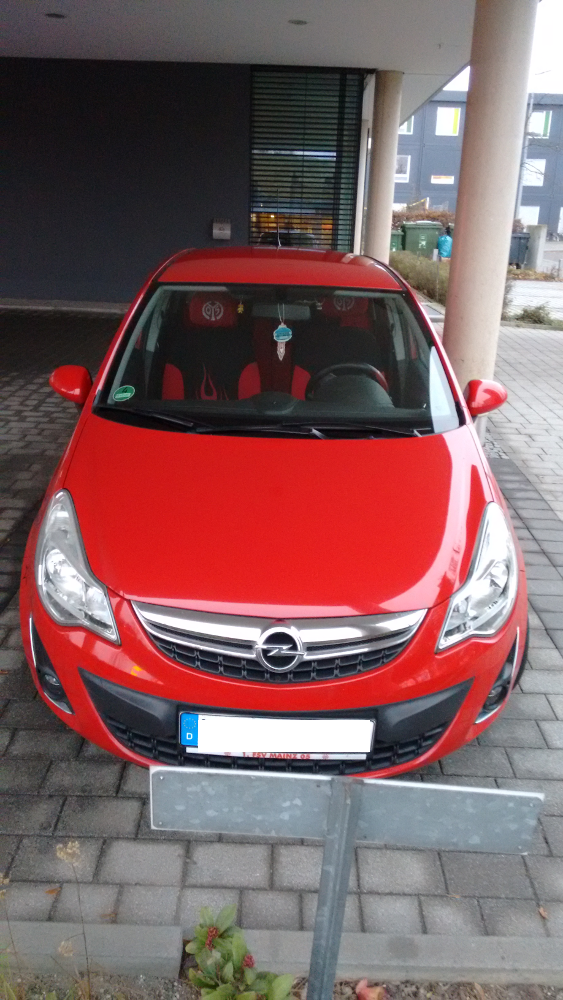
\includegraphics[height=.25\linewidth]{gfx/test4}} \\
        \subfloat[Golf IV]
        {\label{fig:test5}%
         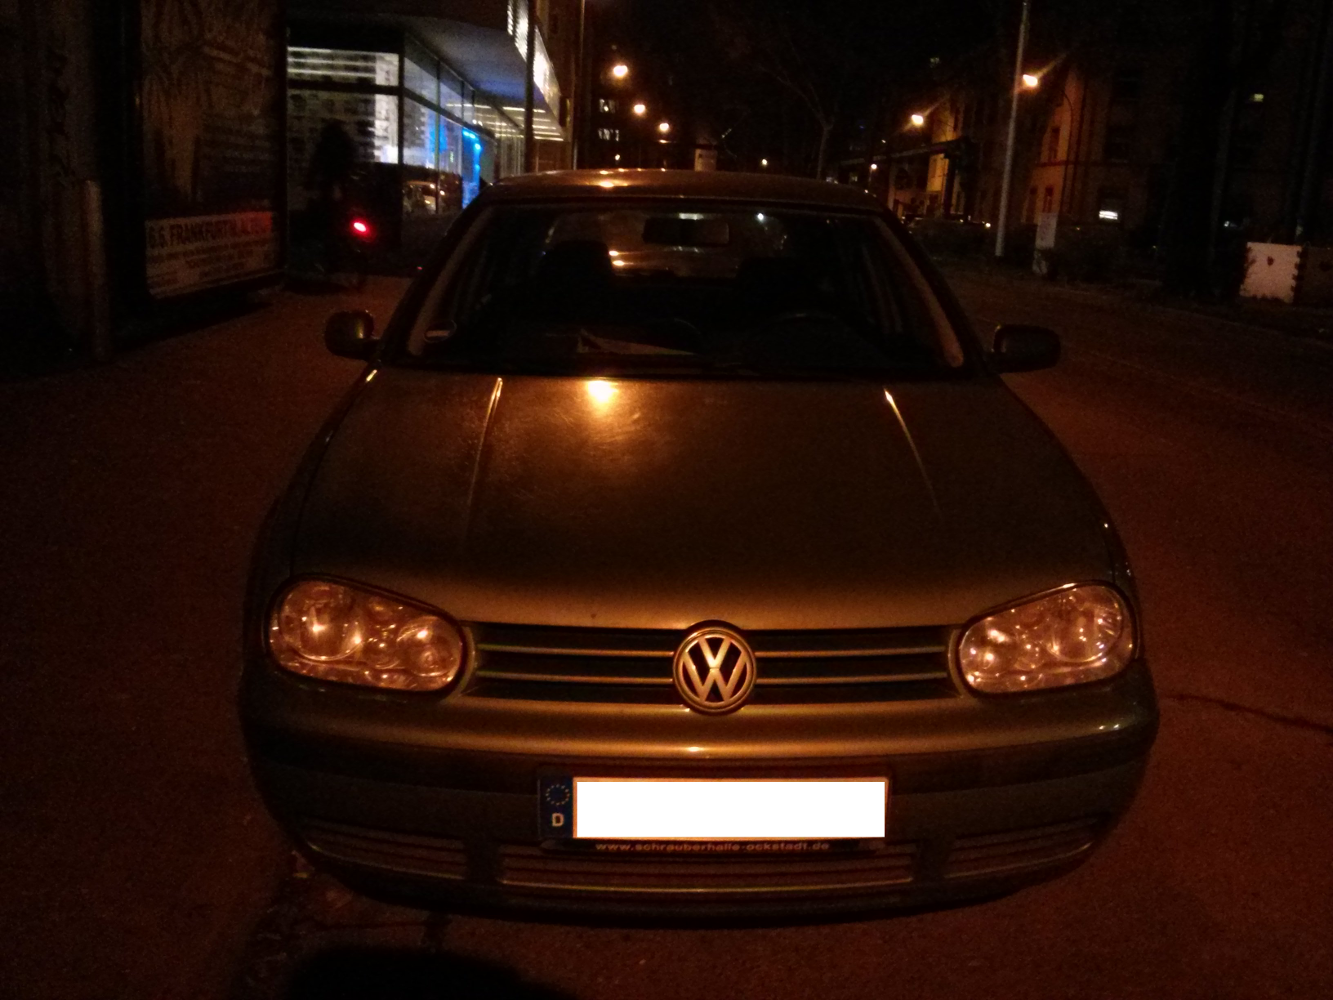
\includegraphics[height=.2\linewidth]{gfx/test5}} \quad
        \subfloat[Golf IV]
        {\label{fig:test6}%
         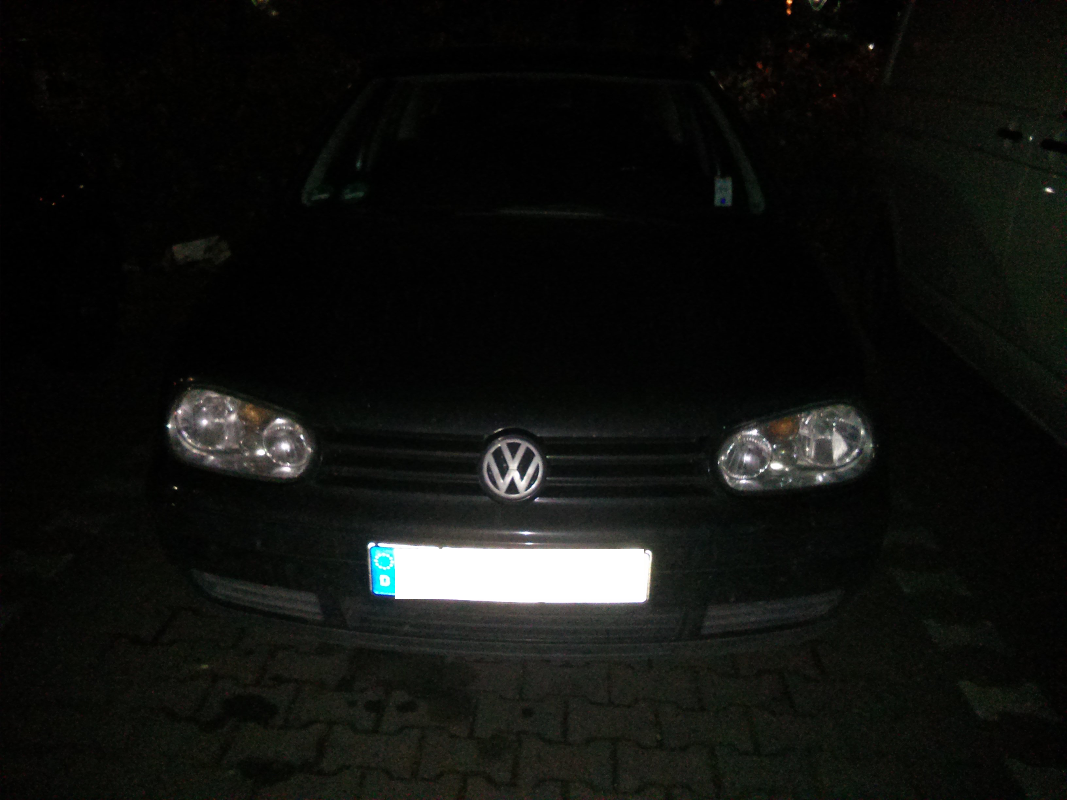
\includegraphics[height=.2\linewidth]{gfx/test6}} \quad
        \subfloat[Tesla Model S]
        {\label{fig:test7}%
         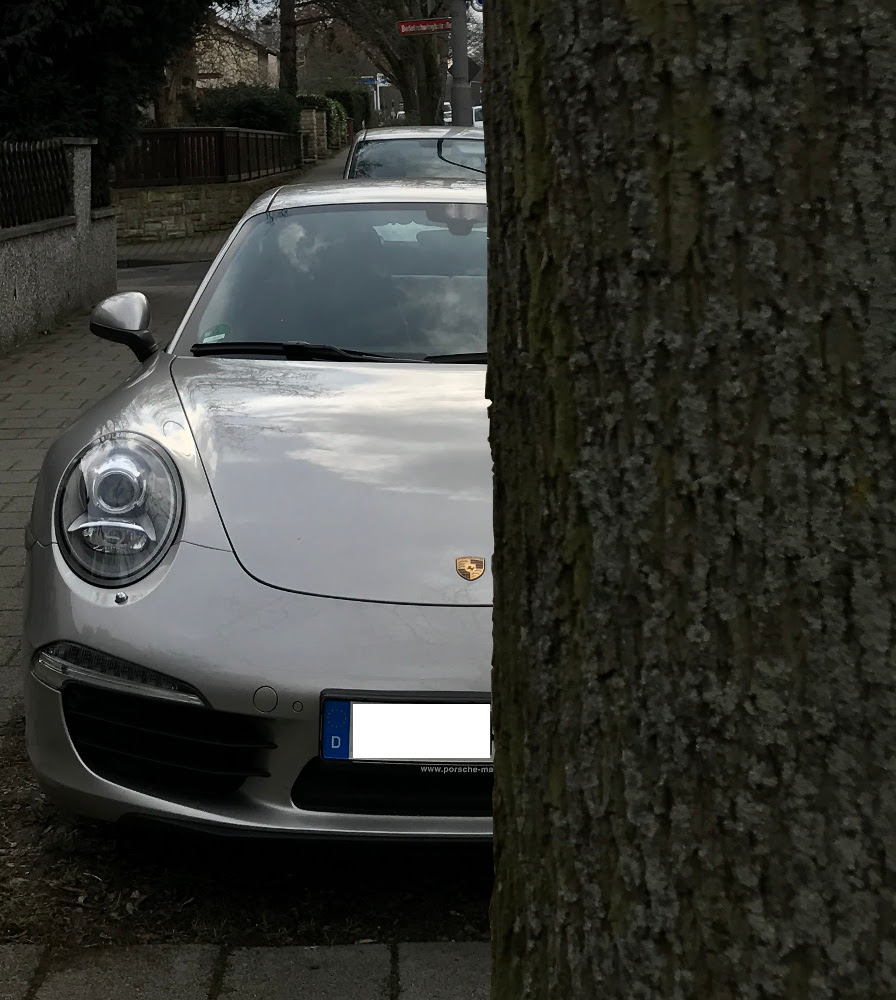
\includegraphics[height=.2\linewidth]{gfx/test7}} \quad
        \subfloat[VW Polo 9N3]
        {\label{fig:test8}%
         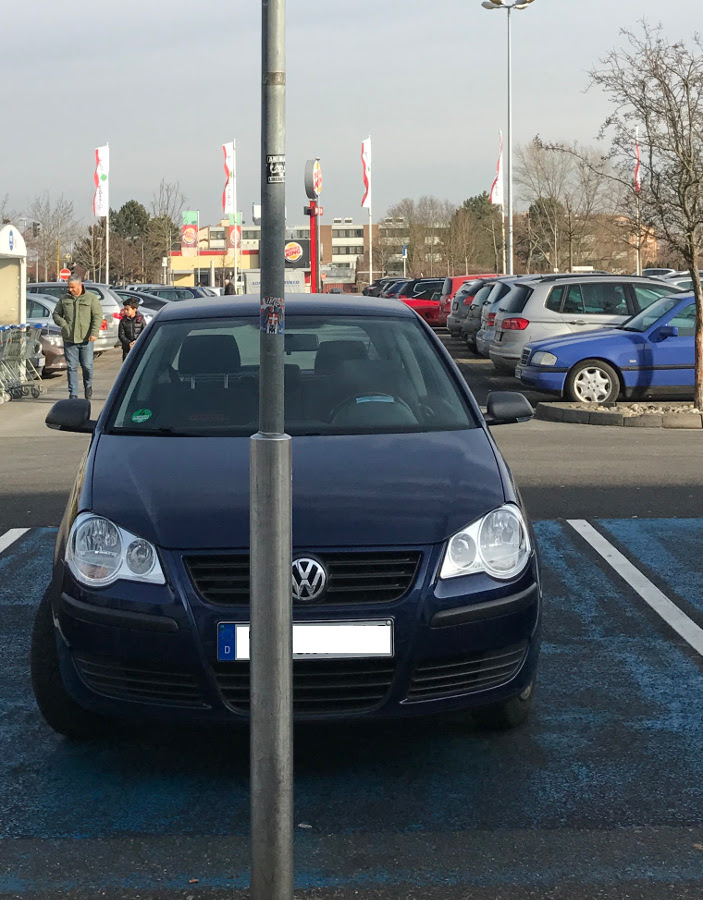
\includegraphics[height=.2\linewidth]{gfx/test8}}
        \caption[Classification results (shown as caption of each picture) in problematic scenarios: Only the Porsche (\ref{fig:test7}) has been classified wrongly because of too much occlusion]{Classification results (shown as caption of each picture) in problematic scenarios: Only the Porsche (\ref{fig:test7}) has been classified wrongly because of too much occlusion}
\label{fig:tests}
\end{figure}

\subsubsection{Ambiguity and Multiplicity}
Despite of the selection of the $N_c = 10$ optimal matching classes out of the total classes from the training set, there exist ambiguity issues among these classes. E. g. the VW K\"afer is often classified as a Porsche 991 and vice versa. Even the classifier recognizes the common origin of these two vehicles.

Additionally, the VW New Beetle (see figure \ref{fig:testAmbiguity}) is classified as a VW K\"afer, although only the classic generation from the 60s and 70s has been trained. For a VMMR that only knows a couple of make-models, this is a welcome side effect due to inter-class ambiguity. Whereas for the final version of the game, this is an unwanted behavior, because the price the car dealer pays for a rare classic VW K\"afer is much higher than for a rather common VW New Beetle.

The inter-class ambiguity issue due to a rebadging of a vehicle is not solved by this VMMR (see chapter \ref{sec:excursionAmbiguity} and figure \ref{fig:ambiguityRebadging}). The changes between the original and the rebadged vehicle are usually too marginal. For the game RacecAR GO, this is not a big problem, because the worth and the property-set of the original and the rebadged vehicle usually do not differ, so the player wouldn't be bothered about a wrong classification. Whereas for a surveillance application, this is a more severe issue.
\begin{figure}[btph]
  \centering
        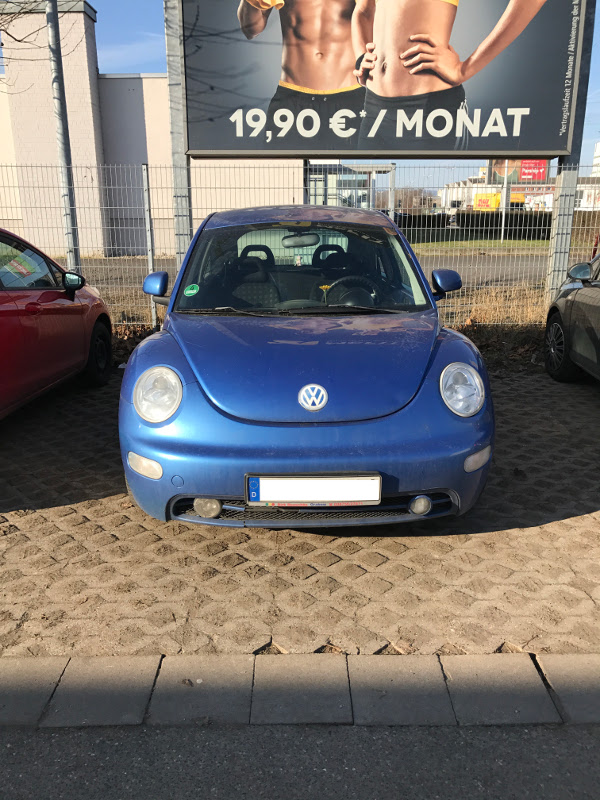
\includegraphics[width=.2\linewidth]{gfx/test_ambiguity}
        \caption{VW New Beetle is classified as a VW K\"afer}
        \label{fig:testAmbiguity}
\end{figure}

If the VMMR accuracy, the robustness to different lighting conditions and to occlusion is good enough to keep the players motivated, will be evaluated during the testing phase (see chapter \ref{ch:evaluation}), when RacecAR GO is played in a real-world environment.


\section{Network Interface}\label{sec:network}
For the transmission of data, TCP sockets are used. In comparison to e. g. HTTP, the protocol is lean and only the needed data is sent. Additionally, the server application is independent of a web server.

For the VMMR request, the whole RoI pixels are transmitted to the server. To just recognize the make and model and to keep the message size low, the normalized global representation histogram (4 bytes * 500 = 2 kB instead of 400 * 190 bytes = 76 kB) would be enough. For this, the client would have to do the feature detection and extraction as well as building the global representation out of the learned dictionary. This has some drawbacks:
\begin{itemize}
  \item The client has to know the dictionary, which makes it hard to improve the dictionary without updating the app
  \item The client-side feature detection and extraction has to work the same way as it has been done to train the VMMR machine. Since the server and the client are implemented in different languages, this is not so easy to assure (actually, it's possible, as long as e. g. OpenCV is used, which is available for both, a Java and an iOS environment).
\end{itemize}
So the decision was made to send the whole RoI and leave the complete recognition process to the server. For evaluation purposes, also the player name and location data is transmitted to the server. In table \ref{table:network}, the network protocol is listed.
\begin{table}[btph]
  \centering
  \begin{tabular}{|p{0.15\textwidth}|p{.3\textwidth}|p{0.3\textwidth}|}
	\hline
	\textbf{Message Type} & \textbf{Request Payload} & \textbf{Response Payload} \\ \hline
	%%%
	VMMR &
	\begin{itemize}
	\item number of rows
	\item number of columns
	\item RoI pixels
	\end{itemize} &
	\begin{itemize}
	\item error status
	\item make-model
	\end{itemize} \\ \hline
	%%%
	Player Name &
	\begin{itemize}
	\item length of name
	\item name
	\end{itemize} &
	\emph{nothing} \\ \hline
	%%%
	Location &
	\begin{itemize}
	\item latitude
	\item longitude
	\end{itemize} &
	\emph{nothing} \\ \hline
  \end{tabular}
  \caption{Network protocol used in the RacecAR GO prototype}
  \label{table:network}
\end{table}


\section{Client}\label{sec:clientImpl}
The client has been implemented as an iOS app for iPhones. Here, OpenCV was used as well for the extraction of the RoI. Used languages are Swift, Objective-C and C++, while latter was only needed to communicate with the OpenCV API. Objective-C was used for the image capturing component because of having trouble when trying to do this with Swift. The rest and thus the main part of the client is implemented in Swift 2.3.

\subsection{Virtual Models}
Although there are ten different make-models to be recognized by the VMMR machine, only four different virtual models have been created for lack of time. Three of them to fit the exact recognized make and model, a further one to be a placeholder for all the other classes. Figure \ref{fig:virtualModels} shows the created 3D models, available for the prototype\footnote{While the Polo, the K\"afer and the Placeholder Car have been created by myself, the Porsche has been retrieved and adapted from \url{https://www.cgtrader.com/free-3d-models/car/sport/porsche-911-carrera-s4-police-concept}}.

\begin{figure}[btph]
        \myfloatalign
        \subfloat[VW Polo 9N3]
        {\label{fig:test1}%
         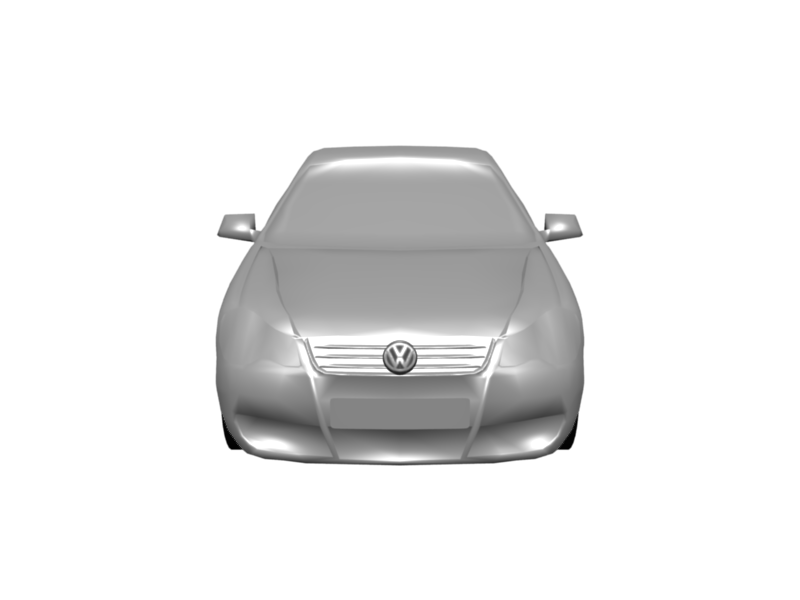
\includegraphics[height=.15\linewidth]{gfx/icon_vw_polo_9n3}} \quad
        \subfloat[VW K\"afer]
        {\label{fig:test2}%
         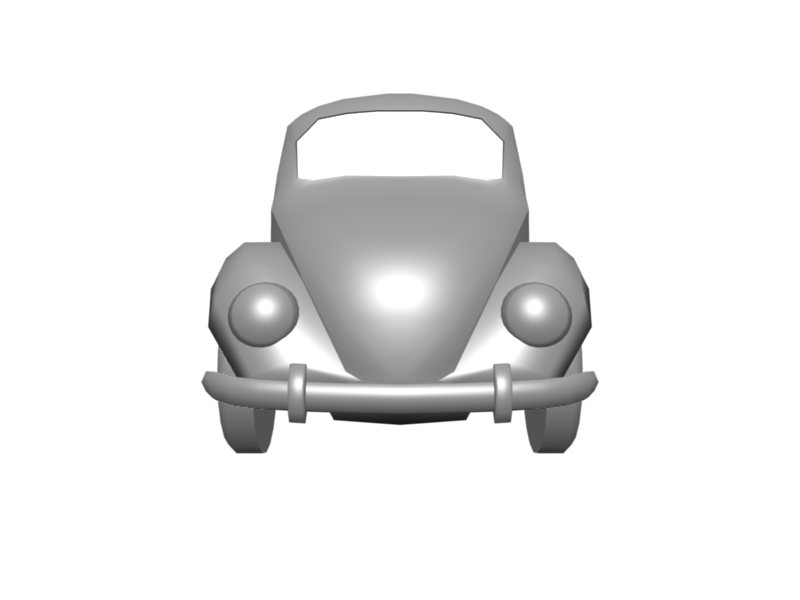
\includegraphics[height=.15\linewidth]{gfx/icon_vw_kaefer}} \quad
        \subfloat[Porsche 911]
        {\label{fig:test3}%
         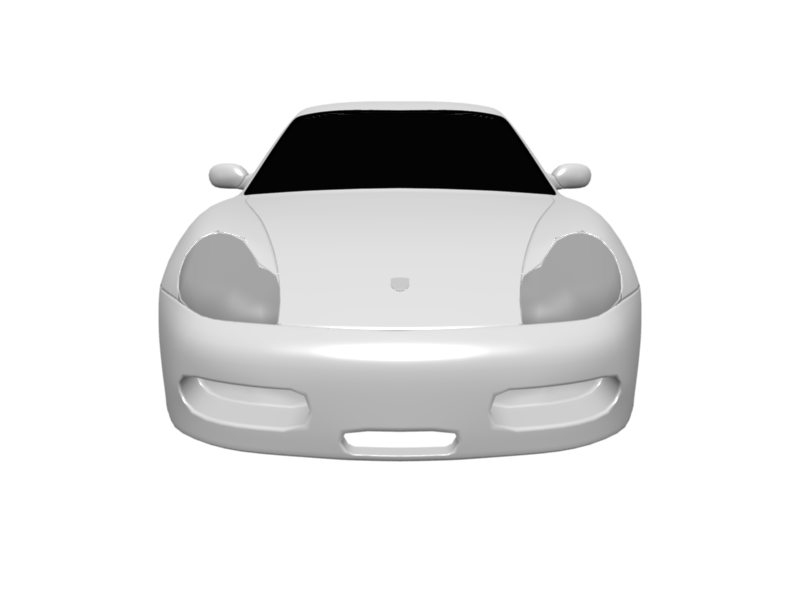
\includegraphics[height=.15\linewidth]{gfx/icon_porsche_911}} \quad
        \subfloat[Placeholder Car]
        {\label{fig:test4}%
         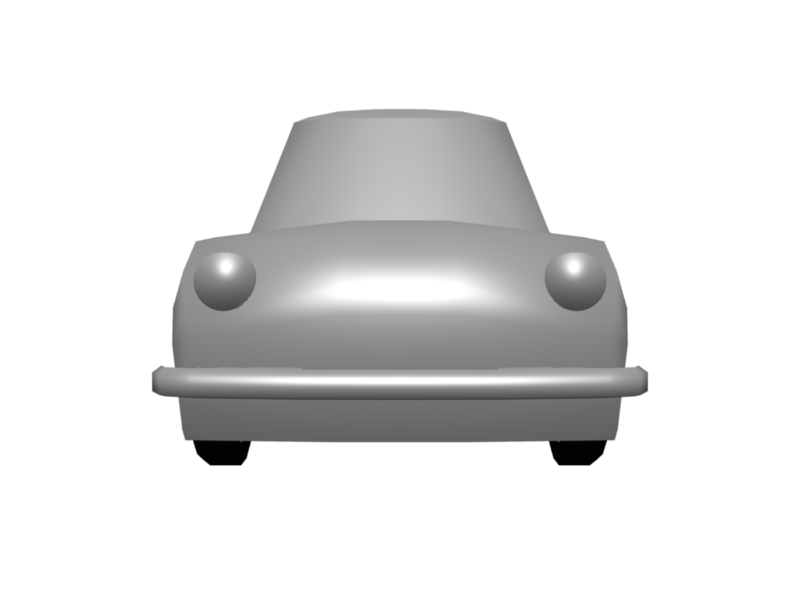
\includegraphics[height=.15\linewidth]{gfx/icon_placeholder_car}}
        \caption[Virtual 3D models to be used in the prototype. Actually, the virtual model for the Porsche 911 is the generation 996, whereas only the newest generation 991 has been trained]{Virtual 3D models to be used in the prototype. Actually, the virtual model for the Porsche 911 is the generation 996, whereas only the current generation 991 has been trained}
\label{fig:virtualModels}
\end{figure}

\subsection{Capturing Process}
In figure \ref{fig:capturingScreenshots}, the capturing process, as it looks like in the game, is illustrated with screenshots. The first one (\ref{fig:capturing1}) displays the view after entering the capturing mode. The entire display (except for the navigation bar) is covered with the camera capture. In the lower third of the screen, there's the watermark, which has to cover the real number plate (displaced a bit in the screenshot for better visibility).

Since the smartphone's motion sensors are used to retrieve the correct pose for AR, the device's \texttt{initialAttitude} is saved when pressing the capture-button (and the RoI around the number plate watermark is transmitted to the server). To retrieve the attitude, the \texttt{CMMotionManager} of the \texttt{CoreMotion} component is used. With this, updates to the device's attitude can be tracked regularly. As soon as the make-model is returned from the server (\ref{fig:capturing2}), the client loads the respective 3D model and property-set (both stored client-side). The 3D model is rendered above the camera capture, while the pose of the virtual camera is deduced from the current device's attitude as
\begin{verbatim}
  camera.pose = currentAttitude.pose * inverse(initialAttitude.pose)
\end{verbatim}
In virtual camera-space, the 3D model is placed at that position, where the real car is expected to be at time of capturing. So leaving the camera in place after capturing will blend the 3D model above the expected real-world vehicle's position. Changing the pose of the smartphone (i. e. of the smartphone's camera) also means changing the pose of the virtual camera, which moves the virtual vehicle along with the real-world vehicle. This works well, as long as solely the orientation of the smartphone is changed. Because of too great inaccuracies, the location changes of the smartphone are not transferred to the virtual camera.

\begin{figure}[btph]
        \myfloatalign
        \subfloat[Placing the watermark]
        {\label{fig:capturing1}%
         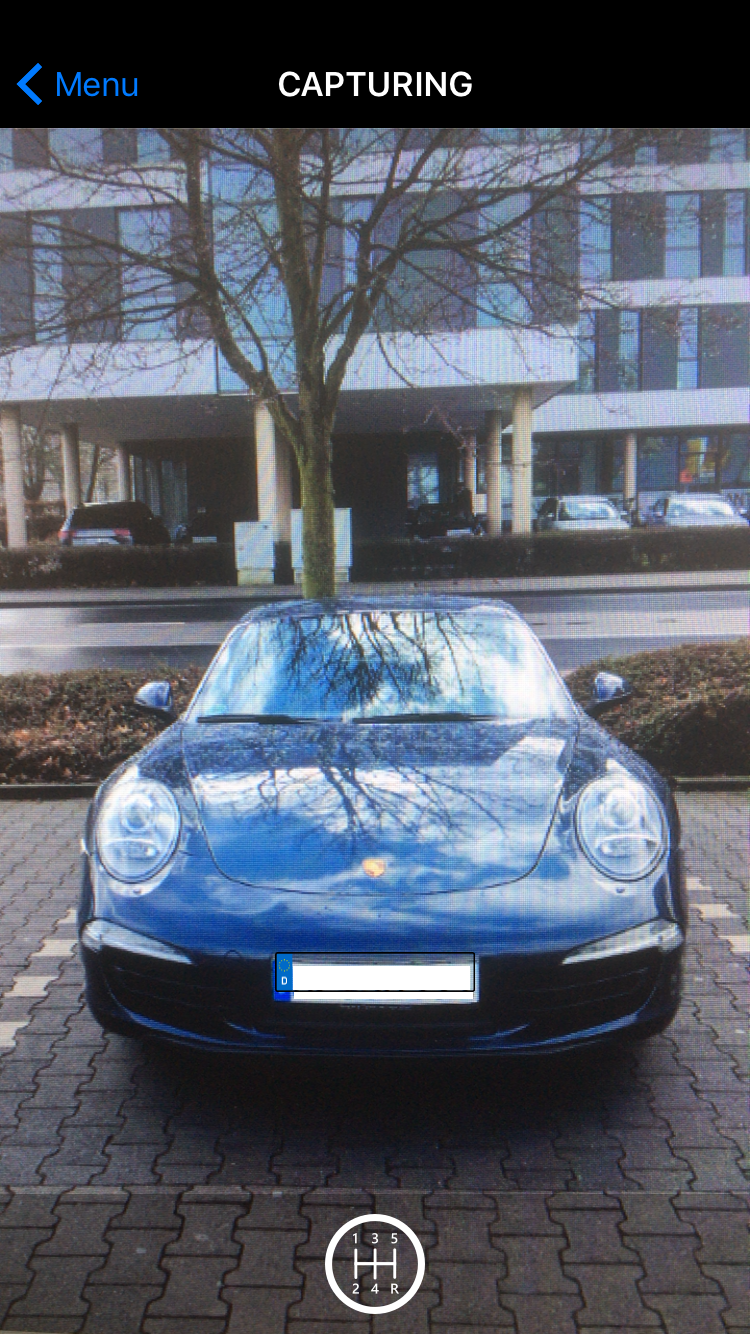
\includegraphics[height=.4\linewidth]{gfx/racecar_go_capturing1}} \quad
        \subfloat[AR with recognized make-model]
        {\label{fig:capturing2}%
         \includegraphics[height=.4\linewidth]{gfx/racecar_go_capturing2}} \quad
        \subfloat[Garage]
        {\label{fig:capturing3}%
         \includegraphics[height=.4\linewidth]{gfx/racecar_go_garage}} \quad
        \subfloat[Play Card]
        {\label{fig:capturing4}%
         \includegraphics[height=.4\linewidth]{gfx/racecar_go_play_card}}
        \caption[Screenshots from RacecAR GO illustrating the capturing process. (a) Capturing the real-world vehicle and placing the watermark. (b) AR overlay of the 3D model. (c) Garage, where all captured vehicles are listed. (d) Selecting one vehicle from the Garage shows that vehicle as a play card, as it would be used in the Supertrumpf game]{Screenshots from RacecAR GO illustrating the capturing process. (a) Capturing the real-world vehicle and placing the watermark. (b) AR overlay of the 3D model. (c) Garage, where all captured vehicles are listed. (d) Selecting one vehicle from the Garage shows that vehicle as a play card, as it would be used in the Supertrumpf game}
\label{fig:capturingScreenshots}
\end{figure}

\subsection{Location Data}\label{sec:locationTracking}
To evaluate the players' movement, the app also transmits location data to the server. This is only done, when the app is currently running and only with permission of the user. Location updates are sent in five meters distance steps. Although more accurate data is available and could be logged, it is not necessary for the evaluation. The location of the iPhone is retrieved by the \texttt{CLLocationManager} of the \texttt{CoreLocation} component. It allows to get continuous updates of the latitude and longitude.





%*****************************************************************************
%*****************************************************************************
\chapter{Evaluation}\label{ch:evaluation}
%*****************************************************************************
%*****************************************************************************
\begin{figure}[btph]
        \myfloatalign
        {\label{fig:eval1}%
         \includegraphics[height=.3\linewidth]{gfx/eval1}} \quad
        {\label{fig:eval2}%
         \includegraphics[height=.3\linewidth]{gfx/eval2}} \quad
        {\label{fig:eval3}%
         \includegraphics[height=.3\linewidth]{gfx/eval3}} \quad
        {\label{fig:eval4}%
         \includegraphics[height=.3\linewidth]{gfx/eval4}} \quad
        \caption[Photos taken during a testing session]{Photos taken during a testing session}
\end{figure}
The purpose of this thesis was to investigate, if real-world vehicles are suited to be used as anchors in an exergame. So an evaluation has been done, including a test phase of the RacecAR GO prototype in the real world.

For this reason, questions in the following domains were examined: The first domain is the adaptation of the game in different environments, such as urban and rural areas. One of the decisive reasons to pick real-world vehicles as anchors was their availability all over the world. So this domain is an important one. Another domain is the integration of the game into their players' everyday life. As this is a focus of pervasive games, answers to this allow to draw conclusions about the pervasive qualities of the game. Correspondingly, the immersion effect of the game and how AR benefits this was evaluated. To investigate the game's strengths in motivating people to move, there are some questions concerning this domain as well as location data, tracked by the app. In more detail, players have been asked before and after the test phase, which distance they walk weekly and if they consider themselves as athletic. It is additionally evaluated, if especially the hunting and collecting of items was a motivator. Since the gameplay requests the player to photograph other people's properties, and since playing mobile games in the public is not easy for anyone, the counter-motivational factor of embarrassment was examined. The recognition accuracy as perceived by the user is also evaluated. And because hazards accompanying a game that is played outside are such a big issue since Pok\'{e}mon GO came out, it was investigated if RacecAR GO also has the potential to cause hazardous moments.

\section{Evaluation Setup}
17 people with ages from eight to 56 years took part at the evaluation, three of them are females. 12 of them had the app installed on their own iPhone and tested it during the whole evaluation phase of 21 days. The rest of the testers only played the app once for about an hour. Since RacecAR GO is a single player game for now, each player tested it by himself. Each player was given a short explanation of the gameplay and a list of vehicles, the app was able to recognize.

Additionally, two questionnaires have been prepared, one had to be filled out before, the other one after the testing phase. To match these two questionnaires with the same tester, aliases have been used to keep the answers anonymous. The questions and answers can be found in the appendix of this thesis. Most of the questions had to be answered on a scale with five steps from \emph{1 = yes, absolutely} over \emph{2 = rather yes}, \emph{3 = not sure}, \emph{4 = rather no} to \emph{5 = no, not at all}. RacecAR GO has been built as an iOS app and was spread among the testers\footnote{An iOS app is not so easy to distribute as an Android app. For a distribution, a membership to the Apple Developer Program is necessary, and this is not for free. So it was done with the iOS Developer University Program of the TU Darmstadt. To finally deploy the app onto the tester's iPhones, \url{https://www.diawi.com/} was used.}.

In addition to the questionnaires, the app itself collects data of the player. This includes the location (see chapter \ref{sec:locationTracking}), the start and end time of each play session and VMMR data. For the VMMR data, each recognition request was logged along with the RoI and the classification result.

The RacecAR GO server was running most of the time during the 21 days of the evaluation phase, whereas in the second week, the VMMR machine has been improved to recognize ten instead of originally seven different make-models.

Within the 21 days, RacecAR GO has been tested in many different urban areas, including the city and suburbs of Mainz, Wiesbaden and Bonn. It was also played in rural environments beyond cities in small villages somewhere in Rheinhessen (evaluated by the tracked GPS data).

\section{Results}
In total, 11.475 km have been traveled with the app during the testing phase. The longest traveled distance during one session was 1.3 km. Each player captured averagely 31 cars during the testing phase. The most vehicles captured by one player are 99. In total, 521 vehicles have been captured. Each tester started the app averagely two times per week and the average duration of one play session was two minutes. The totally played duration is 265 minutes.

There haven't been any noticeable differences between the answers of the long-term and the short-term testers.

The majority of testers (35.3\%) answered the question of the adaptability of RacecAR GO with $3$, further 47\% answered with $1$ and $2$ in equal shares, so they considered the app as adaptive to be playable (nearly) everywhere they wanted to. Only three testers weren't satisfied with the adaptability. These testers, however, had problems to run the app properly on their phones. Although the app may have been playable, because there were some vehicles to capture, 52.9\% of the testers stated that often, the make-models around them weren't covered by the app's VMMR machine. 70\% of the testers reported, that the small number of covered make-models spoiled their enjoyment of the game (rated with 1 and 2 in equal shares).

The ability of the game to be integrated into the everyday life of its players was rated differently. While the majority (35.3\%) rated with \emph{not sure}, 41.1\% of the players found it easy to play the app during their daily routine. This corresponds to the collected data by the app, according to which four testers played the game multiple times at different times of day. 23.6\% of testers found it hard to integrate the game into their everyday lives. A corresponding question has been added to evaluate, if the usual behavior of using the smartphone correlates to this, i. e. a tester that usually hardly uses his smartphone in the daily life may also hardly think of playing the game in his daily life. But the evaluation of this question shows, that this is not the case. While only one tester rather agrees that his sporadic smartphone usage corresponds to the integration problems, most of them (58.8\%) voted, that they not at all didn't think of playing the game because of their infrequent smartphone usage.

When using AR (or fancy technology in general), game designers can fall into the trap of concentrating too much on that technology and neglect the gameplay (as discussed on page \pageref{sec:usageOfARStateOfTheArt}). The testers, however, did not find, that the AR effects distracted them from the actual gameplay. While just one tester voted with a $2$ (when $1$ means, that AR absolutely distracted from the gameplay), the rest voted with $3$ (35.3\%), $4$ (17.6\%) and $5$ (41.2\%). Considering that the AR overlay does not have a direct purpose in the prototype, this is an acceptable result.  In contrast to that, no player was absolutely satisfied with the accuracy of the overlaying effect. Nevertheless, the majority (70.6\%) voted with $2$ and $3$. So on balance, this is an acceptable result for a rather simple implementation of the overlaying effect. In section \ref{sec:motivationToMove} it was supposed that the capturing process including the AR effects could help the players to build an emotional relation to the caught item and thus motivate them to keep playing. In fact, many testers (41\%) answered this question with \emph{not at all}, whereas one player was absolutely able to build an emotional relation and anyway 29.4\% felt \emph{rather able} to build an emotional relationship.

If the app did actually motivate the testers to move has been evaluated in many ways. For one thing, the players have been asked beforehand, which distance they walk weekly and if they think, that the app will motivate them to walk even more. For another thing, the tracked location data and the answers of the questionnaire after the test phase help to comprehend, if the app was actually motivating people to move more than before. Sadly, no tester exceeded the weekly distance, he specified before the test phase (at least not with the running app). But there is one more tester absolutely considering himself as athletic in comparison to before the test phase. The drop of bitterness is, that the number of testers, that considered themselves as not at all athletic increased from one to three. The answers to the question, if a tester moves more than before, now, confirms this. Most of them voted with \emph{no} (70.6\%), whereas only 11.8\% voted with \emph{rather yes}. Conclusively it could be said, that the app has the potential to motivate some people to move. But as long as the players get frustrated because of the few supported make-models, this motivator is only short-lived. It has also been assumed, that hunting and collecting could be a motivator, which cannot be approved by the evaluation. Most testers (41.2\%) weren't sure for this question and only 5.9\% and 23.5\% voted with \emph{yes, absolutely} and \emph{rather yes}, respectively. However, the hunting for especially cars seems to be even more interesting for people. 17.6\% voted with \emph{yes, absolutely} and 29.4\% with \emph{rather yes}.

The factor of embarrassment is not negligible for this game. Whereas the majority (52.9\%) voted with $3$ for the embarrassment of being watched by bystanders while playing the game, 64.7\% of testers voted with \emph{yes} for finding it embarrassing to photograph other people's cars. Especially, there was no tester finding this not at all embarrassing. There was even one case, in which a car owner was angry about his car being photographed.

The rating of the VMMR speed was rather good, most of the testers (88.2\%) rated with \emph{no} or \emph{not sure} for that the recognition took too long. In contrast to that, all testers voted with $1$ to $3$, that it was annoying that cars haven't been classified correctly. An explanation for this could be, that many testers aren't at home in the subject of cars (64.7\% specified to like cars). So many of them weren't able to differentiate between cars that are covered by the VMMR and cars that aren't. The good thing is, that the testers were totally undeterred by that and just captured any car they wanted to possess in their virtual garage. Since most of those cars did not belong to the list of covered cars, testers became disappointed. Vehicles from the list of covered make-models have usually been classified correctly. An outlier is the Ford Fiesta, that has never been classified correctly while totally eight capturing attempts have been made. An explanation for that is its bad true positive rate (cf. table \ref{table:classificationResults}).

Although RacecAR GO has the potential to cause hazardous situations (see chapter \ref{sec:hazards}), most of the testers did not feel unsafe while playing it. 70.6\% answered with \emph{not at all}, no one answered with \emph{yes, absolutely}. Additionally, during the whole testing phase, no hazardous situations occurred.
\begin{figure}[btph]
  \centering
        \includegraphics[width=.95\linewidth]{gfx/eval5}
        \caption{Photo showing a tester having captured a VW Polo with RacecAR GO}
        \label{fig:eval5}
\end{figure}

A secondary aim of the app was to give the players an understanding of cars. For this reason, the testers have been asked before and after the testing phase, if they like cars. Before the tests, 23.5\% absolutely liked cars, whereas 41.2\% rather liked cars. After the tests, still 23.5\% of testers (also the same persons) absolutely like cars but sadly the percentage of testers rather liking cars decreased to only 17.6\%. These 17.6\% of testers voted the same before the test. So the app did not reach the aim to make the players more like cars. Instead, some of the testers don't like cars anymore. One tester even switched from a rating of \emph{rather yes} to \emph{not at all}. Nevertheless, one tester told me afterwards, that she is now much more conscious about cars, when she's on the way.

The testers also had the possibility to mention things they like and things they don't like about the app. Most of the testers wrote, that they like the idea of capturing cars and finding them in one's virtual garage afterwards. Others like the capturing process, the integration of the real world and the correct recognition of make-models. One tester remarked, that he enjoyed an innocuous game without violence.

One thing, nearly all testers do not like, is the support of too few different make-models. Another point of criticism was the placement of the number plate watermark, which requires a steady hand.

%TODO: Am Ende dann ein paar interessante Correlationen plotten, wie: Leute, die sich für unsportlich halten, sind am weitesten gelaufen, oder Non-Autofans haben die meisten Autos gecapturt.
%Gibt es einen Fall, wo ein Non-Autofan nach dem Spiel einer ist? Oder andersrum?
%Einfluss von schon mal Ingress oder Pokemon GO gespielt?

\section{Lessons Learned}
The game is headed in the right direction. After all, the question if the app has finally not only been played to do me a favor was answered with \emph{rather yes} by three generous testers. Additionally, most testers reported, they would like to play the game, if more different make-models were supported.

The evaluation of the questionnaire and the tracked data as well shew, that less that the half of the testers found it easy to integrate the app into their everyday lives. Hence the app lacks some kind of reminder. From personal experiences, sending push messages at the right time can remind the users to play the game. On the other hand, sending push messages at the wrong time could annoy people, such that they play the game even less. The art of finding a good moment to remind the player to play instead of annoying him has been investigated in the app Twostone, which was described in chapter \ref{sec:locationBasedGames}. A motivating reminder could be for example: "Attention! Two other players recently captured a Porsche 911 50 meters away. Go and catch it, too!".

The testers also found a bug\footnote{A bug denotes a malfunction of computer software.} in the VMMR system: The recognition done by a tall person works worse that done with a smaller person. This could be due to an overfitting of the classifier because of training data with too little diversity. The training images, although taken by different persons, were all taken from the same point of view, more or less. This is, because all training data collectors are about 1.75 meters tall. So the VMMR system only learned to classify vehicle pictures taken by 1.75 meters tall people. As a solution, the training images per class need to have more diversity in the point of view.

One thing, inseparably linked to using vehicles as natural anchors is the necessity of photographing other people's cars. The evaluation shew, that the embarrassment, that comes along with this, is a more or less big problem for each of the testers.





%*****************************************************************************
%*****************************************************************************
\chapter{Conclusion}\label{ch:conclusion}
%*****************************************************************************
%*****************************************************************************



%TODO: Auswertungsdiagramme von Google Forms dann auch in Appendix, zusammen mit den Fragen.

%\nocite{*} % invisibly cite all that is in the bib file! (not a good idea, only for demonstration purposes!)


%*****************************************
%*****************************************
%*****************************************
%*****************************************
%*****************************************